\part{模型无关性}
\chapter{换模型函子}\label{ch:change-of-model-functors}


\providecommand{\Fun}{\operatorname{Fun}}
\providecommand{\QCat}{\mathcal{Q}\mathcal{C}at}
\providecommand{\CSS}{\mathcal{CSS}}

在本章中，我们研究\trInfinityCosmos{}之间的一类\trCosmologicalFunctor，它们
不仅仅保持\trInfinityCategory{}性结构，而且还反射并创造之。我们把这类%
\trFunctor{}称作\emph{\trCosmologicalBiequivalence}，因为它们在诸%
\trHomotopyTwoCategory{}之间诱导的\trTwoFunctor{}是\emph{\trBiequivalence}：
对象在\trEquivalence{}意义下满，并且在诸\trHomCategory{}上定义%
\trLocalEquivalence。非正式地，我们把\trCosmologicalBiequivalence{}称作
「\trChangeOfModel{}」\trFunctor。例如，\cref{exa:cosmoi-models} 中引入的那
四个 $(\infty,1)$-\trCategory{}的\trInfinityCosmos{}就由下列%
\trBiequivalence{}相互连接——它们在\cref{exa:biequivalences-models} 中得到
简要的描述，并在附录 E.2 中被重新访问：

\rvsync{1}%
\begin{rveq}\label{eq:four-model-cosmoi}
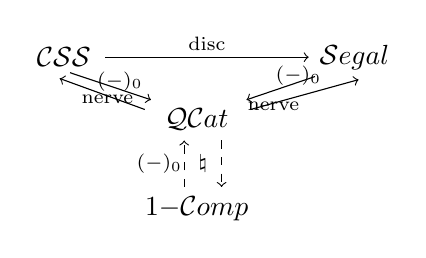
\begin{tikzpicture}[x=1.5em,y=1.4em]
  \node (CSS)   at (0,2.6)    {$\CSS$};
  \node (Segal) at (7.0,2.6)  {$\mathcal{S}egal$};
  \node (QCat)  at (3.2,1.0)  {$\QCat$};
  \node (Comp)  at (3.2,-1.3) {$1\text{-}\mathcal{C}omp$};
  \draw[->] (1.0,2.6) -- (5.9,2.6);
  \node at (3.45,2.95) {$\scriptstyle\mathrm{disc}$};
  \draw[->] (0.15,2.2) -- (2.1,1.5);
  \node at (1.35,1.98) {$\scriptstyle(-)_0$};
  \draw[->] (1.95,1.25) -- (-0.1,2.05);
  \node at (1.05,1.5) {$\scriptstyle\mathrm{nerve}$};
  \draw[->] (6.05,2.1) -- (4.4,1.5);
  \node at (5.65,2.12) {$\scriptstyle(-)_0$};
  \draw[->] (4.5,1.25) -- (7.1,2.02);
  \node at (5.05,1.32) {$\scriptstyle\mathrm{nerve}$};
  \draw[->,dashed] (2.9,-0.75) -- (2.9,0.45);
  \node at (2.3,-0.15) {$\scriptstyle(-)_0$};
  \draw[->,dashed] (3.8,0.45) -- (3.8,-0.75);
  \node at (3.35,-0.15) {$\scriptstyle\natural$};
\end{tikzpicture}
\end{rveq}

在 10.1 节中，我们把散见于全书各处的关于\trCosmologicalFunctor{}的若干结果
汇集在一起。在 10.2 节中，我们重新引入\trBiequivalence{}这一特殊类别，并
讨论一般的例子。特别地，我们将发现：第 6 章的∞-宇宙论在\trBiequivalence{}之下
不变——例如，一个\trCosmologicalBiequivalence{}
$\mathcal{K}\Rightarrow\mathcal{L}$ 诱导一个\trCosmologicalBiequivalence{}
$\mathcal{C}art(\mathcal{K})\Rightarrow\mathcal{C}art(\mathcal{L})$。

由于诸\trInfinityCosmos{}之间的\trBiequivalence{}被要求是%
\trCosmologicalFunctor——有似于富集的右 Quillen 伴随——「对之容许一个%
\trBiequivalence」这一关系并不对称。于是，当我们说两个\trInfinityCosmos{}
「是\trBiequivalence{}的」时，我们意谓：存在一条由\trBiequivalence{}构成的
有限之字形链把两者连接起来；换言之，在由\trCosmologicalBiequivalence{}之
存在所定义的那一关系的对称\trTransitiveClosure{}之下，它们位于同一个%
\trEquivalence{}类中。
特别地，按此定义，一个\emph{$(\infty,1)$-\trCategory{}的\trInfinityCosmos}
是指这样一个\trInfinityCosmos：它经由一条由\trCosmologicalBiequivalence{}构成
的有限之字形链，与 \eqref{eq:four-model-cosmoi} 中的任何一个\trInfinityCosmos
相连接。在这一特殊情形，\cref{prop:underlying-qcat-biequivalence} 建立了一个更简单的刻画，证明一个%
\trInfinityCosmos{} $\mathcal{K}$ 是一个 $(\infty,1)$-\trCategory{}的%
\trInfinityCosmos，当且仅当\trUnderlyingQuasiCategory{}函子
$(-)_0\coloneqq\Fun(1,-)\colon\mathcal{K}\to\QCat$
是一个\trCosmologicalBiequivalence——这便回溯性地证成了%
\cref{def:cosmos-of-infinity-one-categories}。

在 10.3 节中，我们建立\trBiequivalence{}的基本 2-范畴性质，这为第 11 章中的%
\trModelIndependence{}结果的证明提供一个本质性的要素。最后，在 10.4 节中，
我们探讨为\trCosmologicalBiequivalence{}形式地定义的「逆」之诸性质。这些
「逆」不保证是\trCosmologicalFunctor，甚至不保证是通常严格意义下的%
\trSimplicialFunctor。情势与 2-范畴论相类似：定义一个\trBiequivalence{}的%
\trTwoFunctor{}容许一个逆\trBiequivalence，但后者可能只是一个\emph{伪函子}
（pseudofunctor）——这一概念在\cref{def:pseudofunctor} 中被重温。因此，%
\trCosmologicalBiequivalence{}之逆定义一个「拟范畴富集的伪函子」，或简称
\emph{拟伪函子}（quasi-pseudofunctor）：它虽不是宇宙论的，却确实定义一个%
\trBiequivalence，并且使得复合而成的诸\trEndofunctor{}皆与每个\trInfinityCosmos{}上的
恒等函子\emph{拟伪自然等价}（quasi-pseudonaturally equivalent）。这些结构将
在第 12 章中重现，作为在相互\trBiequivalence{}的诸\trInfinityCosmos{}之间
搬运解析地定义的诸结构之工具。

\providecommand{\rvCorner}[1]{\ulcorner #1\urcorner} %

\section{宇宙论函子再访}\label{sec:cosmological-functors-revisited}

请回忆\cref{def:cosmological-functor}：\textbf{\trCosmologicalFunctor}是诸%
\trInfinityCosmos{}之间的一个\trSimplicialFunctor{} $F\colon\mathcal{K}\to\mathcal{L}$，
它保持
\begin{itemize}
\item 指定的诸\trIsofibration{}类，以及
\item 全部宇宙论\trLimit。
\end{itemize}
\cref{lem:cosmological-preserves-equivalences}表明，\trCosmologicalFunctor{}还%
保持诸\trEquivalence{}与诸\trTrivialFibration{}。由\cref{prop:flexible-weights-homotopical}(i)，
\trCosmologicalFunctor{}还保持全部\trFlexibleWeightedLimit。

\trCosmologicalFunctor{}的例子比比皆是——例如见\cref{prop:cosmological-functor-constructions}，
以及 6.3 节中构造的诸充盈子\trInfinityCosmos{}之\trCosmologicalEmbedding。
还有一些\trCosmologicalFunctor{}，连接着以\trInverseCategory{}为指标的\trFibrant\trDiagram{}之%
诸\trInfinityCosmos{}（见练习 6.1.iii），例如

定义域\trFunctor、余定义域\trFunctor{}与恒同\trFunctor
\begin{center}
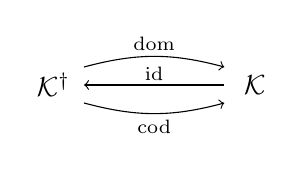
\begin{tikzpicture}[x=1.3em,y=1.3em]
  \node (Kd) at (0,0) {$\mathcal{K}^{\dagger}$};
  \node (K) at (5.6,0) {$\mathcal{K}$};
  \draw[->] (0.85,0.5) to[bend left=15] (4.75,0.5);
  \node at (2.8,1.15) {$\scriptstyle\mathrm{dom}$};
  \draw[->] (4.75,0) -- (0.85,0);
  \node at (2.8,0.32) {$\scriptstyle\mathrm{id}$};
  \draw[->] (0.85,-0.5) to[bend right=15] (4.75,-0.5);
  \node at (2.8,-1.15) {$\scriptstyle\mathrm{cod}$};
\end{tikzpicture}
\end{center}
而\cref{prop:isofibration-cosmos}证明了这些\trFunctor{}是宇宙论的。

\trCosmologicalFunctor{}常常可以限制，从而在平行的充盈子\trInfinityCosmos{}之间%
定义出进一步的\trCosmologicalFunctor：

\begin{lemma}\label{lem:restrict-replete-cosmological}
设 $\mathcal{K}'\hookrightarrow\mathcal{K}$ 与 $\mathcal{L}'\hookrightarrow\mathcal{L}$
是诸充盈子\trInfinityCosmos{}的\trCosmologicalEmbedding。若 $F\colon\mathcal{K}\to\mathcal{L}$
是一个\trCosmologicalFunctor，它把 $\mathcal{K}'$ 的对象与 0-箭头送到
$\mathcal{L}'$ 的对象与 0-箭头，则限制所得的\trFunctor{}是\trCosmological：
\begin{center}
\begin{tikzpicture}[x=1.3em,y=1.3em]
  \node (Kp) at (0,1.2) {$\mathcal{K}'$};
  \node (Lp) at (5.2,1.2) {$\mathcal{L}'$};
  \node (K)  at (0,-1.2) {$\mathcal{K}$};
  \node (L)  at (5.2,-1.2) {$\mathcal{L}$};
  \draw[->,dashed] (0.75,1.2) -- node[above]{$\scriptstyle F$} (4.45,1.2);
  \draw[right hook->] (0,0.7) -- (0,-0.7);
  \draw[right hook->] (5.2,0.7) -- (5.2,-0.7);
  \draw[->] (0.75,-1.2) -- node[below]{$\scriptstyle F$} (4.45,-1.2);
\end{tikzpicture}
\end{center}
\end{lemma}

\begin{proof}
请回忆，\cref{def:replete-subcategory}的充盈性包含如下要求：包含
$\mathcal{K}'\hookrightarrow\mathcal{K}$ 与 $\mathcal{L}'\hookrightarrow\mathcal{L}$
在正维箭头上为满。于是，若\trSimplicialFunctor{} $F$ 把 $\mathcal{K}'$ 的对象与
0-箭头送到 $\mathcal{L}'$ 的对象与 0-箭头，则它限制而定义一个%
\trSimplicialFunctor{} $F'\colon\mathcal{K}'\to\mathcal{L}'$。由于诸%
\trCosmologicalEmbedding{}创造\trIsofibration{}与诸\trCosmologicalLimitNotions，
限制所得的\trFunctor{}是\trCosmological。
\end{proof}

例如，由命题 5.2.4 与练习 5.3.i，\trPullback{}
$f^{*}\colon\mathcal{K}_{/B}\to\mathcal{K}_{/A}$ 保持\trCartesianFibration{}与%
\trCartesianFunctor。于是，沿 $\mathcal{K}$ 中任何\trFunctor{}
$f\colon A\to B$ 的\trPullback{}都限制而定义一个\trCosmologicalFunctor{}（见
命题 7.2.4）：
\begin{center}
\begin{tikzpicture}[x=1.3em,y=1.3em]
  \node (Cl) at (0,1.2) {$\mathcal{C}\mathit{art}(\mathcal{K})_{/B}$};
  \node (Cr) at (7.8,1.2) {$\mathcal{C}\mathit{art}(\mathcal{K})_{/A}$};
  \node (Kl) at (0,-1.2) {$\mathcal{K}_{/B}$};
  \node (Kr) at (7.8,-1.2) {$\mathcal{K}_{/A}$};
  \draw[->,dashed] (Cl) -- node[above]{$\scriptstyle f^{*}$} (Cr);
  \draw[right hook->] (0,0.55) -- (0,-0.55);
  \draw[right hook->] (7.8,0.55) -- (7.8,-0.55);
  \draw[->] (Kl) -- node[below]{$\scriptstyle f^{*}$} (Kr);
\end{tikzpicture}
\end{center}

本节的目标是表明：\trCosmologicalFunctor{}保持我们已引入的全部∞-范畴论结构
——仅有一个值得注意的例外，将在\cref{war:composites-not-preserved}中讨论。
在许多情形下，这一点从原本的 2-范畴式定义（例如定义 5.2.1 中%
\trCartesianFibration{}的定义）来看并不显然，但却可以相当容易地从每个范畴论
概念相配套的「内部刻画」（如定理 5.2.8(ii) 所给者）推出。

重要的是：

\begin{proposition}\label{prop:comma-infinity-categories-preserved}
\trCosmologicalFunctor{}保持\trCommaInfinityCategory：若
$F\colon\mathcal{K}\to\mathcal{L}$ 是一个\trCosmologicalFunctor，且左下图是
$\mathcal{K}$ 中的一个\trCommaCone，则右下图是 $\mathcal{L}$ 中的一个%
\trCommaCone。
\begin{rveq}\label{eq:comma-cone-under-F}
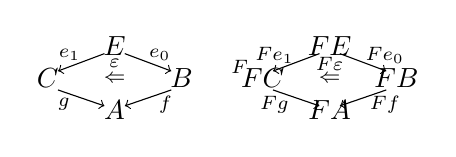
\begin{tikzpicture}[x=1.05em,y=1.05em]
  \begin{scope}
    \node at (0,2.2)    {$E$};
    \node at (-2.3,1.1) {$C$};
    \node at (2.3,1.1)  {$B$};
    \node at (0,0)      {$A$};
    \draw[->] (-0.35,1.95) -- (-1.95,1.35);
    \node at (-1.55,1.9)  {$\scriptstyle e_{1}$};
    \draw[->] (0.35,1.95) -- (1.95,1.35);
    \node at (1.55,1.9)   {$\scriptstyle e_{0}$};
    \node at (0,1.6)      {$\scriptstyle\varepsilon$};
    \node at (0,1.1)      {$\scriptstyle\Leftarrow$};
    \draw[->] (-1.95,0.7) -- (-0.35,0.15);
    \node at (-1.75,0.2)  {$\scriptstyle g$};
    \draw[->] (1.95,0.7) -- (0.35,0.15);
    \node at (1.75,0.2)   {$\scriptstyle f$};
  \end{scope}
  \node at (4.3,1.5)  {$\scriptstyle F$};
  \node at (4.3,0.85) {$\scriptstyle\rightsquigarrow$};
  \begin{scope}[shift={(7.4,0)}]
    \node at (0,2.2)    {$FE$};
    \node at (-2.3,1.1) {$FC$};
    \node at (2.3,1.1)  {$FB$};
    \node at (0,0)      {$FA$};
    \draw[->] (-0.35,1.95) -- (-1.95,1.35);
    \node at (-1.9,1.9)   {$\scriptstyle Fe_{1}$};
    \draw[->] (0.35,1.95) -- (1.95,1.35);
    \node at (1.9,1.9)    {$\scriptstyle Fe_{0}$};
    \node at (0,1.6)      {$\scriptstyle F\varepsilon$};
    \node at (0,1.1)      {$\scriptstyle\Leftarrow$};
    \draw[->] (-1.95,0.7) -- (-0.35,0.15);
    \node at (-1.9,0.2)   {$\scriptstyle Fg$};
    \draw[->] (1.95,0.7) -- (0.35,0.15);
    \node at (1.9,0.2)    {$\scriptstyle Ff$};
  \end{scope}
\end{tikzpicture}
\end{rveq}
\end{proposition}

\begin{proof}
构造\trCommaCone{}的那个单纯\trPullback{} (3.4.2) 为任何\trCosmologicalFunctor{}所保持。
由命题 3.4.11，任何如上方左图所示的\trCommaCone{}都从一支\trFiberedEquivalence
$\rvCorner{\epsilon}\colon E\simeq_{C\times B}\mathrm{Hom}_{A}(f,g)$ 产生，其中
$\epsilon=\phi\rvCorner{\epsilon}$，而任何这种形式的\trFiberedEquivalence{}都%
定义一个\trCommaCone。由于 $F$ 定义一个\trCosmologicalFunctor{}
$F\colon\mathcal{K}_{/C\times B}\to\mathcal{L}_{/FC\times FB}$，故有
$F\rvCorner{\epsilon}\colon FE\simeq_{FC\times FB}F(\mathrm{Hom}_{A}(f,g))\cong\mathrm{Hom}_{FA}(Ff,Fg)$，
于是我们得出结论：右图的数据同样定义一个\trCommaCone。
\end{proof}

利用\cref{prop:comma-infinity-categories-preserved}，我们可以迅速确立%
\trCosmologicalFunctor{}的下列保持性质。为便于查检，这张清单也把在别处确立的
保持性质一并收入。

\begin{proposition}\label{prop:cosmological-preservation-properties}
\trCosmologicalFunctor{}保持：
\begin{enumerate}[label=(\roman*)]
\item \trInfinityCategory{}之间的\trEquivalence。
\item 可逆\trNaturalTransformation{}与对应。
\item \trInfinityCategory{}之间的\trAdjunction，包括右伴随右逆伴随与左伴随
  右逆伴随。
\item \trFiberedAdjunction{}与\trFiberedEquivalence。
\item \trIsofibration、\trTrivialFibration{}与\trDiscrete{}\trInfinityCategory。
\item \trFlexibleWeightedLimit。
\item \trCommaSpan{}与\trCommaCone。
\item \trAbsoluteRightLifting{}图表与\trAbsoluteLeftLifting{}图表。
\item 以\trSimplicialSet{}为指标的\trDiagram{}之\trLimit{}或\trColimit，
  以及保余极限/保极限的\trFunctor。
\item \trStable{}\trInfinityCategory{}与\trExactFunctor。
\item \trCartesianFibration{}与\trCocartesianFibration，以及其间的%
  \trCartesianFunctor。
\item \trDiscreteCartesianFibration{}与\trDiscreteCocartesianFibration。
\item \trTwoSidedFibration，以及其间的\trCartesianFunctor。
\item \trModule{}与可表示模。
\end{enumerate}
\end{proposition}

\begin{proof}
由\cref{lem:simplicial-functor-2-functor}，一个\trCosmologicalFunctor{}诱导诸%
\trHomotopyTwoCategory{}之间的一个 2-\trFunctor，而任意的 2-\trFunctor{}都保持
(i)、(ii) 与 (iii) 的诸结构（例如见引理 2.1.3）。由于\trCosmologicalFunctor{}在
诸\trSliceInfinityCosmos{}之间诱导\trCosmologicalFunctor，(iv) 可以理解为
(i) 与 (iii) 的特例。

\trTrivialFibration{}的保持已由\cref{lem:cosmological-preserves-equivalences}
确立，而\trDiscrete{}\trInfinityCategory{}的保持随之得出（见%
\cref{rem:cosmological-discrete-categories}）。\cref{prop:flexible-weights-homotopical}(i)
证明\trCosmologicalFunctor{}保持全部\trFlexibleWeightedLimit，即 (vi) 所述。
\cref{prop:comma-infinity-categories-preserved}证明\trCosmologicalFunctor{}保持%
\trInfinityCosmos{}中的\trCommaSpan{}与\trHomotopyTwoCategory{}中的\trCommaCone，
即 (vii) 所述。

保持性质 (viii) 最先见于推论 3.5.7，它由定理 3.5.3（该定理把绝对提升图表刻画
为逗号∞-范畴之间的\trFiberedEquivalence）、\cref{prop:comma-infinity-categories-preserved}
（它说\trCosmologicalFunctor{}保持诸逗号）以及「\trCosmologicalFunctor{}保持诸%
\trEquivalence」这一事实得出。(ix) 则由这一点、定义 2.3.8 以及「%
\trCosmologicalFunctor{}保持单纯\trTensor」这一事实得出，其中关于保余极限/
保极限\trFunctor{}的陈述由 (ii) 得出。由定理 4.4.12(iii)，(x) 可以理解为
(ix) 的特例。

保持性质 (xi) 与 (xii) 也由\cref{prop:comma-infinity-categories-preserved}得出
——经由定理 5.2.8(ii)、定理 5.3.4(ii) 与命题 5.5.8 的诸刻画，加上「%
\trCosmologicalFunctor{}保持右或左伴随右逆伴随、对应与\trTrivialFibration」
这一事实。更多细节见推论 5.3.5 的证明；该证明还观察到，笛卡尔自然变换亦为%
\trCosmologicalFunctor{}所保持。

直接从定理 7.1.4 的内部刻画以及伴随与可逆\trNaturalTransformation{}的保持出发，
可得：\trCartesianFunctor{}保持\trTwoSidedFibration{}与其间的\trCartesianFunctor，
如推论 7.1.8 所观察。这就确立了 (xiii)。由\cref{prop:cosmological-functor-constructions}(vi)，
一个\trCosmologicalFunctor{}在诸\trSliceInfinityCosmos{}之间诱导一个直像%
\trCosmologicalFunctor，后者再由 (v) 保持离散对象。于是，\trModule{}也被保持。
把\cref{prop:comma-infinity-categories-preserved}特化到含恒同的\trCospan，
立见左可表示逗号与右可表示逗号被保持。由于一支\trModule{}是可表示的，当且仅当
它与其中之一纤维化等价，可表示\trModule{}也随之被保持——这就完成了 (xiv) 的
证明。
\end{proof}

\begin{warning}\label{war:composites-not-preserved}
在\trCosmologicalFunctor{}所保持的∞-范畴论结构清单中，显著缺席者是模的%
\trVirtualEquipment{}中的诸复合，以及参照这一概念而定义的种种进一步结构：
\trExactSquare、逐点右\trExtension{}与左\trExtension，以及以∞-范畴为指标的%
\trDiagram{}之（加权）\trLimit{}与\trColimit。

复合与强复合一般不为\trCosmologicalFunctor{}所保持，这背后有多种因素。一个
立即可见的问题出自定义 8.3.1 与定义 8.3.5 所给的诸\trUniversalProperty：
其中每一条都涉及全称量词。由于\trCosmologicalFunctor{}未必\trEssentiallySurjective，
定义域中的全称量词未必辖及余定义域。

在另一些语境中，全称量词可以借诸∞-范畴论概念的「内部刻画」而免除，但本情形
没有给出这样的刻画。症结在于这样一个事实：复合的\trModule{}应当理解为借一个
「拉回稳定的逐纤维余反转器」而定义，这一构造把由诸\trSpan{}之复合构成的%
\trTwoSidedFibration{}反射为\trDiscrete{}双侧纤维化。我们未曾给出这样的构造，
因为我们关于\trInfinityCosmos{}的公理化概念不包含余极限；但即便包含——而且
题外话 E.1.8 表明，∞-范畴的\trHomotopyColimit{}在诸例子中常常存在——%
\trCosmologicalFunctor{}由于其「类右伴随」的品性，也不会保持它们。

话虽如此，凡由应用引理 8.3.7 而得的强复合都为\trCosmologicalFunctor{}所保持，
因为\trFiberedAdjunction{}被保持。这包括 8.3 节与 8.4 节所确立的全部形式地定义的复合。
类似的评论也适用于\trExactSquare。由于一般的复合不为\trCosmologicalFunctor{}所
保持，一般的\trExactSquare{}也未必被保持。但 9.2 节所确立的形式地定义的诸%
\trExactSquare{}为\trCosmologicalFunctor{}所保持。例如，\cref{lem:comma-squares-exact}
证明：\trCommaSquare{}在任何\trInfinityCosmos{}中都是\trExactSquare。由于%
\trCosmologicalFunctor{}保持\trCommaSquare，这一类\trExactSquare{}便随之被保持。

正如我们将发现的，\trCosmologicalBiequivalence{}\emph{确实}保持全部这些
∞-范畴论概念，而且还反射并创造它们。我们现在就转向这一主题。
\end{warning}

\subsection*{练习}

\begin{exercise}\label{ex:sliced-fib-cosmos-functor}
请论证：任何\trCosmologicalFunctor{} $F\colon\mathcal{K}\to\mathcal{L}$ 都对
$\mathcal{K}$ 中的每一对\trInfinityCategory{} $A$ 与 $B$ 诱导一个%
\trCosmologicalFunctor{}
$F\colon{}_{A}\mathcal{F}\mathit{ib}(\mathcal{K})_{/B}\to{}_{FA}\mathcal{F}\mathit{ib}(\mathcal{L})_{/FB}$。
\end{exercise}

\begin{exercise}\label{ex:reflected-created-properties}
练习 6.3.iv 表明，\trCosmologicalEmbedding{}在保持\trDiscrete{}\trInfinityCategory{}%
之外还反射它们。\trCosmologicalEmbedding{}还反射或创造哪些其他的∞-范畴论性质？
\end{exercise}

   %
\providecommand{\Fun}{\operatorname{Fun}}
\providecommand{\QCat}{\mathcal{Q}\mathcal{C}at}

\section{宇宙论双等价}\label{sec:cosmological-biequivalences}

特殊的\trCosmologicalFunctor{}——诸\trBiequivalence{}——反射并创造本书所%
发展的∞-范畴论，同时也保持之。请回忆定义 1.3.8：一个\textbf{\trCosmologicalBiequivalence}是一个\trCosmologicalFunctor{} $F\colon\mathcal{K}\to\mathcal{L}$，它
\begin{itemize}
\item 依等价意义于对象上为满：对所有 $C\in\mathcal{L}$，存在 $A\in\mathcal{K}$%
使得 $FA\simeq C$；并且
\item 是诸\trQuasiCategory{}之间的一个\trLocalEquivalence：对每一对 $A$ 与 $B\in\mathcal{K}$，映射
\begin{equation*}
\Fun(A,B)\xrightarrow{\ \sim\ }\Fun(FA,FB)
\end{equation*}
是诸\trQuasiCategory{}之间的一个\trEquivalence。
\end{itemize}

本节中，我们继续追寻\trCosmologicalBiequivalence{}的更多例子。下一节中，我们%
将探讨它们作为\trChangeOfModel{}\trFunctor{}的角色。

例如，\eqref{eq:four-model-cosmoi} 中的那些\trFunctor{}都是\trBiequivalence%
（见\cref{exa:biequivalences-models}与附录 E.2）。除\trFunctor{}%
$\natural\colon\QCat\to 1\text{-}\mathcal{C}omp$ 之外，其余每一个都产生自诸%
\trModelCategory{}之间的一个单纯富集右 Quillen 等价——这些\trModelCategory{}%
富集于全部对象皆余纤维性的 Joyal \trModelStructure{}之上。推论 E.1.2 表明：%
任何这种形式的\trFunctor{}都编码一个\trCosmologicalBiequivalence。

两个\trInfinityCosmos{}是\textbf{双等价的}，若存在一条连接两者的、由%
\trBiequivalence{}构成的有限之字形链。请回忆：任何\trInfinityCosmos{}都有一个\trUnderlyingQuasiCategory{}函子
\begin{equation*}
\mathcal{K}\xrightarrow{\ (-)_{0}\coloneqq\Fun(1,-)\ }\QCat
\end{equation*}
它由映出终\trInfinityCategory{}而定义。我们现在证明：任何与 $\QCat$ 双等价的\trInfinityCosmos{}，其\trUnderlyingQuasiCategory{}函子都是一个\trCosmologicalBiequivalence。这便证成了\cref{def:cosmos-of-infinity-one-categories}所给的 \textbf{$(\infty,1)$-\trCategory{}的\trInfinityCosmos}之刻画。

\begin{proposition}\label{prop:underlying-qcat-biequivalence}
若一个\trInfinityCosmos{} $\mathcal{K}$ 与 $\QCat$ 是双等价的，则\trUnderlyingQuasiCategory{}函子 $(-)_{0}\colon\mathcal{K}\Rightarrow\QCat$ 是一个\trCosmologicalBiequivalence。
\end{proposition}

\begin{proof}
我们将证明：当存在\trCosmologicalBiequivalence
\begin{equation*}
\mathcal{K}\xleftarrow[\ \sim\ ]{\ G\ }\mathcal{L}\xrightarrow[\ \sim\ ]{\ F\ }\QCat
\end{equation*}
时，\trUnderlyingQuasiCategory{}函子 $(-)_{0}\colon\mathcal{K}\to\QCat$ 是一个\trCosmologicalBiequivalence。注意这一表述涵盖了 $F$ 或 $G$ 为恒同\trFunctor{}的特殊情形。由归纳法，同样的结论对任何经由一条由\trBiequivalence{}构成的有限之字形链而与 $\QCat$ 相连接的\trInfinityCosmos{}成立。

由于 $F$ 是一个\trBiequivalence，对每个\trQuasiCategory{} $Q$，存在一个\trInfinityCategory{} $B\in\mathcal{L}$ 使得 $FB\simeq Q$。由于 $F$ 与 $G$ 都是保持终\trInfinityCategory{} $1$ 的\trLocalEquivalence——对后者我们在 $\mathcal{K}$、$\mathcal{L}$ 与 $\QCat$ 三者中均沿用同一记号——于是有一条诸\trQuasiCategory{}之\trEquivalence{}构成的之字形链
\begin{equation*}
(GB)_{0}=\Fun(1,GB)\xleftarrow{\ \sim\ }\Fun(1,B)\xrightarrow{\ \sim\ }\Fun(1,FB)\cong FB\simeq Q.
\end{equation*}
这便证明了：存在一个\trInfinityCategory{} $GB\in\mathcal{K}$，其\trUnderlyingQuasiCategory{}等价于 $Q$。

为证\trUnderlyingQuasiCategory{}函子 $(-)_{0}\colon\mathcal{K}\to\QCat$ 是一个\trLocalEquivalence，考虑一对\trInfinityCategory{} $A$ 与 $B\in\mathcal{K}$。由 $G$ 的本质满性，存在\trInfinityCategory{} $X$ 与 $Y\in\mathcal{L}$ 使得 $GX\simeq A$ 且 $B\simeq GY$。经由以这些\trEquivalence{}作\trPreComposition{}与\trPostComposition，推论 1.4.8 蕴含：$\Fun(A,B)\to\Fun(A_{0},B_{0})$ 等价于 $\Fun(GX,GY)\to\Fun((GX)_{0},(GY)_{0})$，故只需证明后一映射是诸\trQuasiCategory{}之间的一个\trEquivalence。

由单纯函子性（见定义 A.2.6），$F$ 与 $G$ 在\trFunctorSpace{}上的作用与复合映射
\begin{equation*}
\Fun(X,Y)\times\Fun(1,X)\xrightarrow{\ \circ\ }\Fun(1,Y)
\end{equation*}
交换，而后者经转置便定义\trUnderlyingQuasiCategory{}函子在\trFunctorSpace{}上%
的作用。于是，有一张竖直映射均为\trEquivalence{}的交换图
\begin{center}
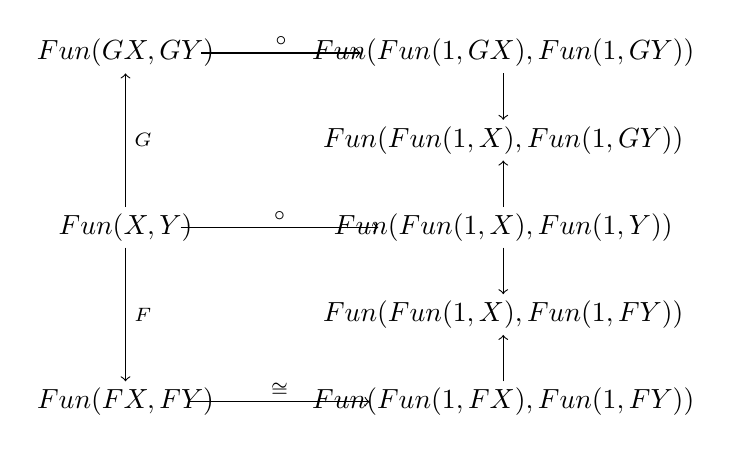
\begin{tikzpicture}[x=1.05em,y=1.05em]
  \node (a) at (0,6)    {$\Fun(GX,GY)$};
  \node (d) at (13,6)   {$\Fun(\Fun(1,GX),\Fun(1,GY))$};
  \node (e) at (13,3)   {$\Fun(\Fun(1,X),\Fun(1,GY))$};
  \node (b) at (0,0)    {$\Fun(X,Y)$};
  \node (f) at (13,0)   {$\Fun(\Fun(1,X),\Fun(1,Y))$};
  \node (g) at (13,-3)  {$\Fun(\Fun(1,X),\Fun(1,FY))$};
  \node (c) at (0,-6)   {$\Fun(FX,FY)$};
  \node (h) at (13,-6)  {$\Fun(\Fun(1,FX),\Fun(1,FY))$};
  \draw[->] (2.6,6) -- (8.1,6);
  \node at (5.35,6.4) {$\scriptstyle\circ$};
  \draw[->] (1.9,0) -- (8.7,0);
  \node at (5.3,0.4) {$\scriptstyle\circ$};
  \draw[->] (2.2,-6) -- (8.4,-6);
  \node at (5.3,-5.6) {$\scriptstyle\cong$};
  \draw[->] (0,0.7) -- (0,5.3);
  \node at (0.6,3) {$\scriptstyle G$};
  \draw[->] (0,-0.7) -- (0,-5.3);
  \node at (0.6,-3) {$\scriptstyle F$};
  \draw[->] (13,5.3) -- (13,3.7);
  \draw[->] (13,0.7) -- (13,2.3);
  \draw[->] (13,-0.7) -- (13,-2.3);
  \draw[->] (13,-5.3) -- (13,-3.7);
\end{tikzpicture}
\end{center}
任何\trQuasiCategory{}都同构于其\trUnderlyingQuasiCategory，故底部水平映射是%
一个\trIsomorphism。由\trTwoOfThreeProperty，顶部水平映射是一个\trEquivalence，这正是我们所要证明的。
\end{proof}

请回忆\cref{prop:cosmological-functor-constructions}(vi)：一个\trCosmologicalFunctor{} $F\colon\mathcal{K}\to\mathcal{L}$ 对任何 $B\in\mathcal{K}$ 都诱导一个\trCosmologicalFunctor{} $F\colon\mathcal{K}_{/B}\to\mathcal{L}_{/FB}$。

\begin{proposition}\label{prop:slice-biequivalence}
若 $F\colon\mathcal{K}\Rightarrow\mathcal{L}$ 是一个\trCosmologicalBiequivalence，则对任何 $B\in\mathcal{K}$，受诱导的\trFunctor{} $F\colon\mathcal{K}_{/B}\Rightarrow\mathcal{L}_{/FB}$ 也是一个\trCosmologicalBiequivalence。
\end{proposition}

\begin{proof}
我们首先论证：$F$ 定义诸\trFunctorSpace{}之间的一个\trLocalEquivalence，如%
命题 1.2.22(ii) 所定义者。给定 $\mathcal{K}$ 中的一对\trIsofibration{} $p\colon E\twoheadrightarrow B$ 与 $p'\colon E'\twoheadrightarrow B$，\trFibered\trFunctorSpace{}上的诱导映射由如下\trPullback{}定义
\begin{center}
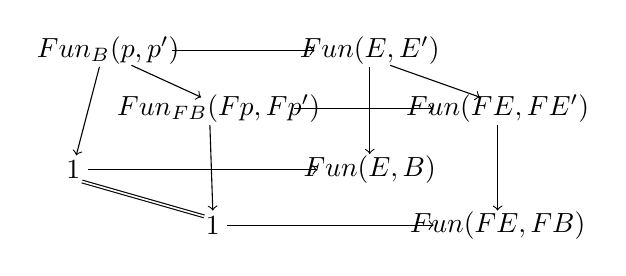
\begin{tikzpicture}[x=1.05em,y=1.05em]
  \node (A) at (-3.8,0)    {$\Fun_{B}(p,p')$};
  \node (C) at (5.2,0)     {$\Fun(E,E')$};
  \node (B) at (0,-2.0)    {$\Fun_{FB}(Fp,Fp')$};
  \node (D) at (9.6,-2.0)  {$\Fun(FE,FE')$};
  \node (I1) at (-5.0,-4.1) {$1$};
  \node (E) at (5.2,-4.1)  {$\Fun(E,B)$};
  \node (I2) at (-0.2,-6.0) {$1$};
  \node (G) at (9.6,-6.0)  {$\Fun(FE,FB)$};
  \draw[->] (-1.6,0) -- (3.3,0);
  \draw[->] (2.6,-2.0) -- (7.4,-2.0);
  \draw[->] (-4.5,-4.1) -- (3.4,-4.1);
  \draw[->] (0.3,-6.0) -- (7.4,-6.0);
  \draw[->] (-3.0,-0.5) -- (-0.6,-1.6);
  \node at (-1.9,-0.75) {$\scriptstyle\rightsquigarrow$};
  \draw[->] (5.9,-0.5) -- (9.0,-1.6);
  \node at (7.4,-0.75) {$\scriptstyle\rightsquigarrow$};
  \draw[->] (-4.1,-0.55) -- (-4.9,-3.6);
  \draw[->] (-0.3,-2.55) -- (-0.2,-5.5);
  \draw[->] (5.2,-0.55) -- (5.2,-3.55);
  \draw[->] (9.6,-2.55) -- (9.6,-5.5);
  \draw[double,double distance=0.6pt] (-4.7,-4.5) -- (-0.5,-5.7);
  \node at (-2.4,-0.85) {$\scriptstyle\lrcorner$};
  \node at (2.7,-2.7) {$\scriptstyle\lrcorner$};
\end{tikzpicture}
\end{center}
由于 $\QCat$ 中诸\trCospan{}之间的映射是\trEquivalence，由命题 3.3.4，诸\trPullback{}之间的诱导映射亦然。

至于在等价意义下的满性：考虑 $\mathcal{L}$ 中的一支\trIsofibration{} $q\colon L\twoheadrightarrow FB$。由于 $F$ 依等价意义于对象上为满，存在某个 $A\in\mathcal{K}$，连同 $\mathcal{L}$ 中的一支\trEquivalence{} $i\colon FA\Rightarrow L$。由于 $F$ 定义诸\trMappingQuasiCategory{}之间的一个\trLocalEquivalence，于是更有 $\mathcal{K}$ 中的一个\trFunctor{} $f\colon A\to B$\footnote{原书印作「a functor $f\colon A\to B$ in $\mathcal{L}$」，按上下文应为「in $\mathcal{K}$」之误（$A$、$B\in\mathcal{K}$，$Ff$ 系 $F$ 在 hom 上的作用），此处径改。——译者注}，使得 $Ff\colon FA\to FB$ 自然同构于 $qi$（见\cref{ex:equivalence-reflects-isomorphism-classes}）。\trFunctor{} $f$ 未必是\trIsofibration，但引理 1.2.19 容许我们把 $f$ 因子分解为 $A\Rightarrow K\twoheadrightarrow B$。选取一支等价逆 $j\colon K\Rightarrow A$，这批数据便定义了 $\mathfrak{h}\mathcal{L}$ 中一个依同构而交换的图表：
\begin{center}
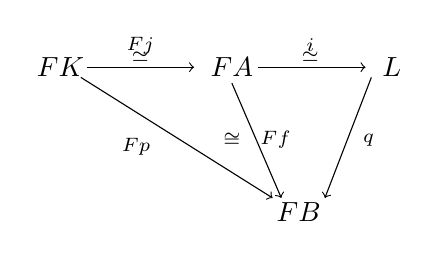
\begin{tikzpicture}[x=1.05em,y=1.05em]
  \node at (0,0)      {$FK$};
  \node at (5.9,0)    {$FA$};
  \node at (11.4,0)   {$L$};
  \node at (8.2,-5.0) {$FB$};
  \draw[->] (0.9,0) -- (4.6,0);
  \node at (2.75,0.75) {$\scriptstyle Fj$};
  \node at (2.75,0.35) {$\scriptstyle\simeq$};
  \draw[->] (6.8,0) -- (10.5,0);
  \node at (8.6,0.75) {$\scriptstyle i$};
  \node at (8.6,0.35) {$\scriptstyle\simeq$};
  \draw[->] (0.7,-0.35) -- (7.3,-4.5);
  \node at (2.6,-2.75) {$\scriptstyle Fp$};
  \draw[->] (5.9,-0.55) -- (7.6,-4.5);
  \node at (5.9,-2.5) {$\scriptstyle\cong$};
  \node at (7.4,-2.5) {$\scriptstyle Ff$};
  \draw[->] (10.7,-0.35) -- (9.1,-4.5);
  \node at (10.6,-2.5) {$\scriptstyle q$};
\end{tikzpicture}
\end{center}

命题 1.4.9 告诉我们：诸\trInfinityCosmos{}中的\trIsofibration{}定义诸\trHomotopyTwoCategory{}中的\trIsofibration。特别地，我们可以沿\trIsofibration{} $q\colon L\twoheadrightarrow FB$ 提升所显示的那个同构，从而定义一个交换的三角形：
\begin{center}
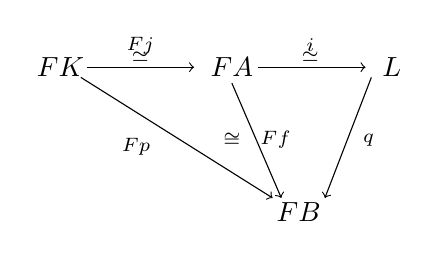
\begin{tikzpicture}[x=1.05em,y=1.05em]
  \node at (0,0)      {$FK$};
  \node at (5.9,0)    {$FA$};
  \node at (11.4,0)   {$L$};
  \node at (8.2,-5.0) {$FB$};
  \draw[->] (0.9,0) -- (4.6,0);
  \node at (2.75,0.75) {$\scriptstyle Fj$};
  \node at (2.75,0.35) {$\scriptstyle\simeq$};
  \draw[->] (6.8,0) -- (10.5,0);
  \node at (8.6,0.75) {$\scriptstyle i$};
  \node at (8.6,0.35) {$\scriptstyle\simeq$};
  \draw[->] (0.7,-0.35) -- (7.3,-4.5);
  \node at (2.6,-2.75) {$\scriptstyle Fp$};
  \draw[->] (5.9,-0.55) -- (7.6,-4.5);
  \node at (5.9,-2.5) {$\scriptstyle\cong$};
  \node at (7.4,-2.5) {$\scriptstyle Ff$};
  \draw[->] (10.7,-0.35) -- (9.1,-4.5);
  \node at (10.6,-2.5) {$\scriptstyle q$};
\end{tikzpicture}
\qquad$=$\qquad
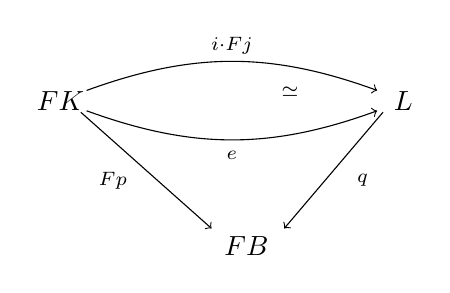
\begin{tikzpicture}[x=1.05em,y=1.05em]
  \node at (0,0)      {$FK$};
  \node at (11.8,0)   {$L$};
  \node at (6.4,-5.0) {$FB$};
  \draw[->] (0.9,0.35) to[bend left=20] (10.9,0.35);
  \node at (5.9,1.9) {$\scriptstyle i\cdot Fj$};
  \node at (7.9,0.3) {$\scriptstyle\simeq$};
  \draw[->] (0.9,-0.35) to[bend right=20] (10.9,-0.35);
  \node at (5.9,-1.9) {$\scriptstyle e$};
  \draw[->] (0.7,-0.4) -- (5.2,-4.4);
  \node at (1.8,-2.75) {$\scriptstyle Fp$};
  \draw[->] (11.1,-0.4) -- (7.7,-4.4);
  \node at (10.4,-2.75) {$\scriptstyle q$};
\end{tikzpicture}
\end{center}
由练习 1.4.iii，由于 $e$ 同构于\trEquivalence{} $i\cdot Fj$，它必定也定义一个\trEquivalence。于是，由命题 1.2.22(vii)，我们已经证明：\trIsofibration{} $p\colon K\twoheadrightarrow B$ 在 $F$ 之下被映射为一支\trIsofibration，后者等价于我们所选的 $q\colon L\twoheadrightarrow FB$。
\end{proof}

类似的论证证明：一个\trCosmologicalBiequivalence{}在\cref{prop:isofibration-cosmos}之相应的诸\trIsofibration{}\trInfinityCosmos{}之间诱导一个\trBiequivalence。

\begin{proposition}\label{prop:dual-biequivalence}
若 $F\colon\mathcal{K}\Rightarrow\mathcal{L}$ 是一个\trCosmologicalBiequivalence，则受诱导的\trFunctor{} $F\colon\mathcal{K}^{\dagger}\Rightarrow\mathcal{L}^{\dagger}$ 是一个\trBiequivalence。\footnote{原书此上标字形经高倍裁片呈 $\natural$/$\sharp$ 族，与 6.1 节之 $\dagger$ 记号不合，孰是存疑；按型义暂从 6.1 节口径排 $\dagger$。——译者注}
\end{proposition}

\begin{proof}
\cref{ex:prove-dual-biequivalence}。
\end{proof}

我们再来确立诸\trSliceInfinityCosmos{}之间的另一族\trBiequivalence：

\begin{proposition}\label{prop:pullback-biequivalence}
若 $f\colon A\Rightarrow B$ 是 $\mathcal{K}$ 中的一个\trEquivalence，则\trPullback\trFunctor{} $f^{*}\colon\mathcal{K}_{/B}\Rightarrow\mathcal{K}_{/A}$ 是一个\trCosmologicalBiequivalence。
\end{proposition}

\begin{proof}
为见 $f^{*}\colon\mathcal{K}_{/B}\to\mathcal{K}_{/A}$ 是\trEssentiallySurjective{}，考虑一个对象 $r\colon D\twoheadrightarrow A$，并用引理 1.2.19 把复合映射 $fr\colon D\to B$ 因子分解为一支\trEquivalence{}后接一支\trIsofibration，再把所得结果沿 $f$ 作\trPullback。
\begin{center}
\begin{tikzpicture}[x=1.05em,y=1.05em]
  \node at (0,0)       {$D$};
  \node at (11.8,-1.5) {$E$};
  \node at (3.6,-5.0)  {$P$};
  \node at (4.5,-10.9) {$A$};
  \node at (11.8,-10.9) {$B$};
  \draw[->] (0.8,0.25) to[bend left=18] (11.2,-1.1);
  \node at (5.8,1.5) {$\scriptstyle\sim$};
  \draw[->,dashed] (0.3,-0.6) -- (3.1,-4.3);
  \draw[->] (5.2,-4.7) -- (10.3,-2.0);
  \node at (7.8,-2.9) {$\scriptstyle\sim$};
  \draw[->] (-0.5,-0.4) to[bend right=12] (3.6,-10.6);
  \node at (0.2,-5.6) {$\scriptstyle r$};
  \draw[->] (3.7,-5.55) -- (4.4,-10.35);
  \node at (4.7,-7.9) {$\scriptstyle q$};
  \draw[->] (11.8,-2.05) -- (11.8,-10.35);
  \node at (12.4,-6.2) {$\scriptstyle p$};
  \draw[->] (6.1,-10.9) -- (10.6,-10.9);
  \node at (8.35,-10.45) {$\scriptstyle\sim$};
  \node at (8.35,-11.4) {$\scriptstyle f$};
  \node at (5.3,-6.1) {$\scriptstyle\lrcorner$};
\end{tikzpicture}
\end{center}
由命题 3.3.3，$f$ 的\trPullback{}是一个\trEquivalence，故由\trTwoOfThreeProperty，$r$ 等价于\trIsofibration{} $q\colon P\twoheadrightarrow A$，后者位于 $f^{*}\colon\mathcal{K}_{/B}\to\mathcal{K}_{/A}$ 的像中。

为证这个单纯\trFunctor{}是\trLocalEquivalence，考虑一对\trIsofibration{} $p\colon E\twoheadrightarrow B$ 与 $q\colon F\twoheadrightarrow B$。我们将证明：在 $B$ 上的\trFunctor{}之\trQuasiCategory{}等价于在它们的\trPullback{}之间、$A$ 上的\trFunctor{}之\trQuasiCategory
\begin{center}
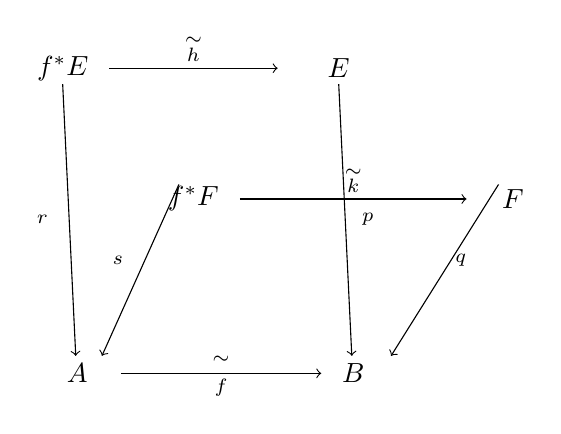
\begin{tikzpicture}[x=1.05em,y=1.05em]
  \node at (0,0)        {$f^{*}E$};
  \node at (9.5,0)      {$E$};
  \node at (4.5,-4.5)   {$f^{*}F$};
  \node at (15.5,-4.5)  {$F$};
  \node at (0.5,-10.5)  {$A$};
  \node at (10,-10.5)   {$B$};
  \draw[->] (1.6,0) -- (7.4,0);
  \node at (4.5,0.45) {$\scriptstyle h$};
  \node at (4.5,0.95) {$\scriptstyle\sim$};
  \draw[->] (6.1,-4.5) -- (13.9,-4.5);
  \node at (10,-4.05) {$\scriptstyle k$};
  \node at (10,-3.6) {$\scriptstyle\sim$};
  \draw[->] (0,-0.55) -- (0.45,-9.9);
  \node at (-0.7,-5.2) {$\scriptstyle r$};
  \draw[->] (4.0,-4.0) -- (1.35,-9.9);
  \node at (1.9,-6.6) {$\scriptstyle s$};
  \draw[->] (9.5,-0.55) -- (9.95,-9.9);
  \node at (10.5,-5.2) {$\scriptstyle p$};
  \draw[->] (15.0,-4.0) -- (11.3,-9.9);
  \node at (13.7,-6.6) {$\scriptstyle q$};
  \draw[->] (2.0,-10.5) -- (8.9,-10.5);
  \node at (5.45,-10.05) {$\scriptstyle\sim$};
  \node at (5.45,-11.0) {$\scriptstyle f$};
  \node at (1.9,-1.1) {$\scriptstyle\lrcorner$};
  \node at (5.9,-5.5) {$\scriptstyle\lrcorner$};
\end{tikzpicture}
\end{center}

为定义比较映射 $\Fun_{B}(E,F)\to\Fun_{A}(f^{*}E,f^{*}F)$，考虑如下交换\trPrism
\begin{center}
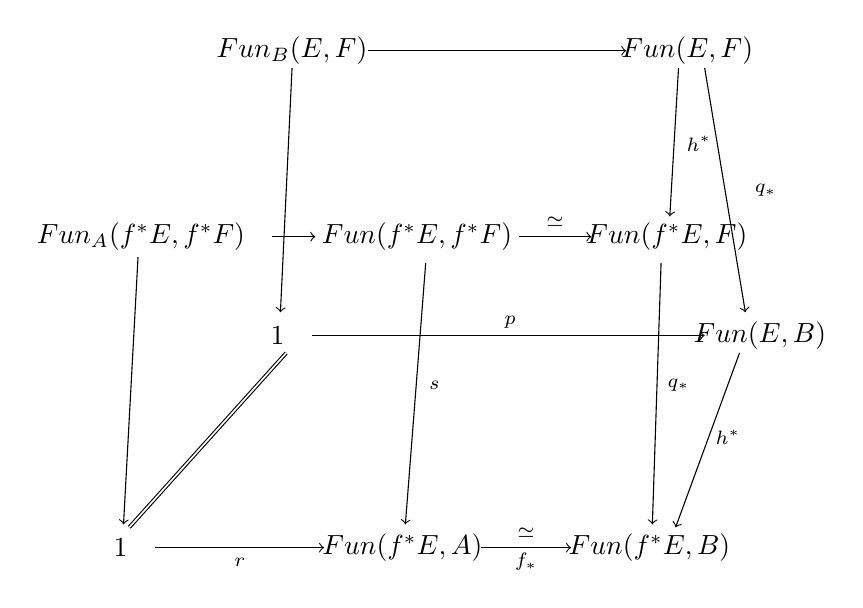
\begin{tikzpicture}[x=1.05em,y=1.05em]
  \node (B1) at (-4.3,7.5)  {$\Fun_{B}(E,F)$};
  \node (T1) at (9.3,7.5)   {$\Fun(E,F)$};
  \node (A1) at (-9.5,1.1)  {$\Fun_{A}(f^{*}E,f^{*}F)$};
  \node (M1) at (0,1.1)     {$\Fun(f^{*}E,f^{*}F)$};
  \node (M2) at (8.6,1.1)   {$\Fun(f^{*}E,F)$};
  \node (Ib) at (-4.8,-2.3) {$\mathbb{1}$};
  \node (TB) at (11.8,-2.3) {$\Fun(E,B)$};
  \node (If) at (-10.2,-9.6) {$\mathbb{1}$};
  \node (MB) at (-0.5,-9.6) {$\Fun(f^{*}E,A)$};
  \node (RB) at (8.0,-9.6)  {$\Fun(f^{*}E,B)$};
  \draw[->] (-1.7,7.5) -- (7.2,7.5);
  \draw[->] (-4.3,6.9) -- (-4.7,-1.5);
  \draw[->] (9.0,6.9) -- (8.7,1.8);
  \node at (9.7,4.3) {$\scriptstyle h^{*}$};
  \draw[->] (9.9,6.9) -- (11.3,-1.5);
  \node at (12.0,2.7) {$\scriptstyle q_{*}$};
  \draw[->] (-5.0,1.1) -- (-3.5,1.1);
  \draw[->] (-9.6,0.4) -- (-10.1,-8.8);
  \draw[->] (3.5,1.1) -- (6.0,1.1);
  \node at (4.75,1.6) {$\scriptstyle\simeq$};
  \draw[->] (0.3,0.2) -- (-0.4,-8.8);
  \node at (0.6,-4.0) {$\scriptstyle s$};
  \draw[->] (8.4,0.2) -- (8.1,-8.8);
  \node at (9.0,-4.0) {$\scriptstyle q_{*}$};
  \draw[->] (-3.6,-2.3) -- (9.9,-2.3);
  \node at (3.2,-1.85) {$\scriptstyle p$};
  \draw[->] (-9.0,-9.6) -- (-3.2,-9.6);
  \node at (-6.1,-10.1) {$\scriptstyle r$};
  \draw[->] (2.2,-9.6) -- (5.3,-9.6);
  \node at (3.75,-9.1) {$\scriptstyle\simeq$};
  \node at (3.75,-10.1) {$\scriptstyle f_{*}$};
  \draw[->] (11.1,-2.9) -- (8.9,-8.9);
  \node at (10.7,-5.8) {$\scriptstyle h^{*}$};
  \draw[double,double distance=0.6pt] (-4.5,-2.9) -- (-9.9,-8.9);
  \node at (-1.8,6.6) {$\scriptstyle\lrcorner$};
  \node at (-5.5,0.3) {$\scriptstyle\lrcorner$};
  \node at (3.6,0.3) {$\scriptstyle\lrcorner$};
\end{tikzpicture}
\end{center}
前右方块由 $f^{*}F$ 的单纯\trUniversalProperty{}成为一个\trPullback，而前左%
方块与背面则是定义
\begin{equation*}
\Fun_{A}(f^{*}E,f^{*}F)\ \text{与}\ \Fun_{B}(E,F)
\end{equation*}
的那些\trPullback。前侧复合\trPullback{}矩形的\trUniversalProperty{}诱导出映射
\begin{equation*}
\Fun_{B}(E,F)\to\Fun_{A}(f^{*}E,f^{*}F)
\end{equation*}
由于这个\trFunctor{}是推论 1.4.8 的那些\trEquivalence{} $h^{*}$ 的\trPullback，由命题 3.3.4，诱导映射定义诸\trQuasiCategory{}之间的一个\trEquivalence。
\end{proof}

更进一步受诱导的\trCosmologicalBiequivalence{}可由应用下述引理产生：该引理%
重访命题 6.3.3 的情形设置——命题 6.3.3 是一个曾用于构造\trCosmologicallyEmbedded{}\trInfinityCosmos{}的结果。我们将其应用留给练习，并在推论 10.3.7 中回到这一话题。

\begin{lemma}\label{lem:pullback-cosmological-biequivalence}
考虑由诸\trInfinityCosmos{}与诸\trCosmologicalFunctor{}构成的一个\trPullback{}图表，其中 $F\colon\mathcal{K}\to\mathcal{L}$ 是一个\trCosmologicalBiequivalence，而 $\mathcal{L}'\hookrightarrow\mathcal{L}$ 与 $\mathcal{K}'\hookrightarrow\mathcal{K}$ 是诸\trCosmologicalEmbedding。\footnote{若 $\mathcal{K}'$ 上的\trInfinityCosmos{}结构是由该\trPullback{}创造的，则 $\mathcal{K}'\hookrightarrow\mathcal{K}$ 自动是一个\trCosmologicalEmbedding，且\trFunctor{} $\mathcal{K}'\to\mathcal{L}'$ 自动是\trCosmological{}（见命题 6.3.3）。}%
\begin{center}
\begin{tikzpicture}[x=1.05em,y=1.05em]
  \node at (0,0)    {$\mathcal{K}'$};
  \node at (6.4,0)  {$\mathcal{L}'$};
  \node at (0,-5)   {$\mathcal{K}$};
  \node at (6.4,-5) {$\mathcal{L}$};
  \draw[->] (0.9,0) -- (5.4,0);
  \node at (3.1,0.45) {$\scriptstyle F$};
  \draw[right hook->] (0,-0.55) -- (0,-4.4);
  \draw[right hook->] (6.4,-0.55) -- (6.4,-4.4);
  \draw[->,double,double distance=0.5pt] (0.9,-5) -- (5.4,-5);
  \node at (3.1,-5.5) {$\scriptstyle F$};
  \node at (2.0,-1.2) {$\scriptstyle\lrcorner$};
\end{tikzpicture}
\end{center}
则 $F\colon\mathcal{K}'\Rightarrow\mathcal{L}'$ 是一个\trCosmologicalBiequivalence。
\end{lemma}

\begin{proof}
要点在于\trCosmologicalEmbedding{} $\mathcal{L}'\hookrightarrow\mathcal{L}$ 的充盈性：它已在\cref{def:replete-subcategory}中被枚举，并在练习 6.3.i 中得到%
探讨。为见 $F\colon\mathcal{K}'\to\mathcal{L}'$ 是\trEssentiallySurjective{}，考虑一个\trInfinityCategory{} $L\in\mathcal{L}'$。由\trCosmologicalBiequivalence{} $F\colon\mathcal{K}\Rightarrow\mathcal{L}$ 的本质满性，存在一个\trInfinityCategory{} $K\in\mathcal{K}$ 使得 $FK\simeq L$（在 $\mathcal{L}$ 中）。由 $\mathcal{L}'\hookrightarrow\mathcal{L}$ 的充盈性，\trEquivalence{} $FK\simeq L$ 也位于 $\mathcal{L}'$ 中，从而 $K$ 位于\trPullback{} $\mathcal{K}'$ 中，并经由 $F$ 被映射到 $\mathcal{L}'$ 中一个与 $L$ 等价的对象。

至于\trLocalEquivalence：与 $\mathcal{K}'$ 中一对\trInfinityCategory{} $A$ 与 $B$ 相关联的\trFunctorSpace{}上的诱导映射构成诸\trQuasiCategory{}的一个\trPullback
\begin{center}
\begin{tikzpicture}[x=1.05em,y=1.05em]
  \node at (0,0)     {$\Fun_{\mathcal{K}'}(A,B)$};
  \node at (14,0)    {$\Fun_{\mathcal{L}'}(FA,FB)$};
  \node at (0,-6.7)  {$\Fun_{\mathcal{K}}(A,B)$};
  \node at (14,-6.7) {$\Fun_{\mathcal{L}}(FA,FB)$};
  \draw[->] (3.1,0) -- (10.4,0);
  \node at (6.75,0.45) {$\scriptstyle F$};
  \draw[right hook->] (0,-0.7) -- (0,-6.0);
  \draw[right hook->] (14,-0.7) -- (14,-6.0);
  \draw[->] (3.6,-6.7) -- (10.4,-6.7);
  \node at (5.4,-6.25) {$\scriptstyle\simeq$};
  \node at (6.75,-7.2) {$\scriptstyle F$};
  \node at (2.0,-1.4) {$\scriptstyle\lrcorner$};
\end{tikzpicture}
\end{center}
由练习 6.3.i，竖直\trFunctor{}是诸\trQuasiCategory{}之间的\trIsofibration。于是，由命题 3.3.3，$F\colon\mathcal{K}\to\mathcal{L}$ 的\trLocalEquivalence{}可作\trPullback{}而定义 $F\colon\mathcal{K}'\to\mathcal{L}'$ 的一个\trLocalEquivalence。故我们断言：限制所得的\trFunctor{}仍是一个\trCosmologicalBiequivalence。
\end{proof}

\subsection*{练习}

\begin{exercise}\label{ex:equivalence-reflects-isomorphism-classes}
（10.3.1）请论证：诸\trQuasiCategory{}之间的一支\trEquivalence{} $f\colon K\Rightarrow L$ 在顶点的同构类上诱导一个双射——亦即，在 $K$ 与 $L$ 的\trHomotopyCategory{}中对象的同构类上诱导一个双射。由此推证：对任何\trCosmologicalBiequivalence{} $F\colon\mathcal{K}\Rightarrow\mathcal{L}$ 与任何一对\trInfinityCategory{} $A$ 与 $B\in\mathcal{K}$：
\begin{enumerate}[label=(\roman*)]
\item 对任何\trFunctor{} $f'\colon FA\to FB$，存在一个\trFunctor{} $f\colon A\to B$ 与一个自然同构 $Ff\cong f'$（在 $\mathcal{L}$ 中）。
\item 若\trFunctor{} $f$ 与 $g\colon A\to B$ 满足：在 $\mathcal{L}$ 中 $Ff\cong Fg$，则在 $\mathcal{K}$ 中 $f\cong g$。
\end{enumerate}
\end{exercise}

\begin{exercise}\label{ex:prove-dual-biequivalence}
证明\cref{prop:dual-biequivalence}。
\end{exercise}

\begin{exercise}\label{ex:slice-cosmoi-biequivalent}
若 $F\colon\mathcal{K}\rightsquigarrow\mathcal{L}$ 是一个\trBiequivalence，且 $A\in\mathcal{K}$ 与 $B\in\mathcal{L}$ 满足 $FA\simeq B$，请证明诸\trSliceInfinityCosmos{} $\mathcal{K}_{/A}$ 与 $\mathcal{L}_{/B}$ 是双等价的。
\end{exercise}

\begin{exercise}\label{ex:biequivalence-invariance}
（10.3.7）请探讨\cref{lem:pullback-cosmological-biequivalence}之于如下任务的适用性：检验 6.3 节所构造的诸\trInfinityCosmos{}在\trBiequivalence{}之下不变。
\end{exercise}

   %
\providecommand{\Fun}{\operatorname{Fun}}
\providecommand{\QCat}{\mathcal{Q}\mathcal{C}at}
\providecommand{\Cat}{\mathcal{C}at}
\providecommand{\hFun}{\mathrm{h}\Fun} %
\providecommand{\HomB}{\mathrm{Hom}_{B}}
\providecommand{\HomFB}{\mathrm{Hom}_{FB}}
\providecommand{\SWarrow}{\rotatebox[origin=c]{-135}{$\Rightarrow$}} %
\providecommand{\Disc}{\mathit{Disc}}
\providecommand{\Stab}{\mathcal{S}\mathit{tab}} %
\providecommand{\Rari}{\mathit{Rari}}
\providecommand{\Lari}{\mathit{Lari}}
\providecommand{\Cart}{\mathcal{C}\mathit{art}}
\providecommand{\CoCart}{\mathit{co}\mathcal{C}\mathit{art}}
\providecommand{\Fib}{\mathcal{F}\mathit{ib}}
\providecommand{\Mod}{\mathbb{M}od}
\providecommand{\hTwoCell}[5]{\tikz[baseline=-0.8ex]{%
  \node (rvl) at (0,0) {$#1$};
  \node (rvr) at (2.9,0) {$#2$};
  \draw[->] (rvl) to[bend left=28] node[above]{$\scriptstyle #3$} (rvr);
  \draw[->] (rvl) to[bend right=28] node[below]{$\scriptstyle #5$} (rvr);
  \node at (1.45,0) {$\scriptstyle #4$};}}

\section{作为换模型函子的宇宙论双等价}\label{sec:cosmological-biequivalences-as-change-of-model-functors}

诸\trInfinityCosmos{}之间的\trBiequivalence{}被称为\trChangeOfModel{}\trFunctor。在本节中，我们列举它们的基本性质。首先，我们观察到\trCosmologicalBiequivalence{}下降为诸\trHomotopyTwoCategory{}之间的\trBiequivalence——名称由此而来：

\begin{proposition}\label{prop:homotopy-two-category-biequivalence}
一个\trCosmologicalBiequivalence{} $F\colon\mathcal{K}\Rightarrow\mathcal{L}$
诱导诸\trHomotopyTwoCategory{}之间的一个\trBiequivalence{}
$F\colon\mathfrak{h}\mathcal{K}\Rightarrow\mathfrak{h}\mathcal{L}$，也就是说，
该 2-\trFunctor
\begin{enumerate}[label=(\roman*)]
\item 依等价意义于对象上为满；并且
\item 对所有 $A$ 与 $B\in\mathcal{K}$，定义诸\trCategory{}之间的一个\trLocalEquivalence
  $\hFun(A,B)\Rightarrow\hFun(FA,FB)$。
\end{enumerate}
\end{proposition}

注意，(ii) 的诸\trLocalEquivalence{}必然具有\cref{ex:equivalence-reflects-isomorphism-classes}所列举的那些性质。

\begin{proof}
由\cref{thm:equivalences-are-equivalences}，∞-宇宙层面的\trEquivalence{}与%
2-\trCategory{}式的\trEquivalence{}相重合，这就证明了 (i)；而由\cref{lem:equiv-homotopy-equivalences}，\trHomotopyCategory{}函子
$\mathrm{h}\colon\QCat\to\Cat$ 把诸\trQuasiCategory{}之间的\trEquivalence{}送到诸\trCategory{}之间的\trEquivalence，这就证明了 (ii)。
\end{proof}

特别地，由此得出：一个\trInfinityCategory{}的\trHomotopyCategory{}在%
\trChangeOfModel{}之下不变（见\cref{ex:homotopy-category-change-of-model}）。更一般地，2-\trCategory{}之间的任何\trBiequivalence{}都诱导出多种局部与整体的双射，如下所列：

\begin{corollary}\label{cor:biequivalence-local-bijections}
考虑任何\trCosmologicalBiequivalence{} $F\colon\mathcal{K}\Rightarrow\mathcal{L}$。
\begin{enumerate}[label=(\roman*)]
\item \trBiequivalence{} $F$ 保持、反射并创造诸\trInfinityCategory{}之间的%
  \trEquivalence，并在对象的\trEquivalence{}类之间定义一个双射。
\item \trBiequivalence{} $F$ 在诸\trFunctor{}的自然\trIsomorphism{}类之间诱导出延伸 (i) 之双射的诸局部双射：选定任何一对对象 $A$ 与 $B\in\mathcal{K}$、
  任何一对 $A'$ 与 $B'\in\mathcal{L}$，以及\trEquivalence
  $a\colon A'\Rightarrow FA$ 与 $b\colon FB\Rightarrow B'$，
  映射
  \begin{rveq}\label{eq:homotopy-categories-map}
  \hFun(A,B)\Rightarrow\hFun(FA,FB)\Rightarrow\hFun(A',B')
  \end{rveq}
  在 $\mathcal{K}$ 中诸\trFunctor{} $A\to B$ 的\trIsomorphism{}类与
  $\mathcal{L}$ 中诸\trFunctor{} $A'\to B'$ 的\trIsomorphism{}类之间定义一个双射。
\item \trBiequivalence{} $F$ 在带指定边界的诸\trNaturalTransformation{}之间定义出延伸 (i) 与 (ii) 之双射的诸局部双射：选定任何一对对象 $A$ 与
  $B\in\mathcal{K}$、任何一对 $A'$ 与 $B'\in\mathcal{L}$、指定的\trEquivalence
  $a\colon A'\simeq FA$ 与 $b\colon FB\simeq B'$、
  诸\trFunctor{} $f$ 与 $g\colon A\to B$ 以及 $f'$ 与 $g'\colon A'\to B'$，还有自然\trIsomorphism
  \begin{center}
  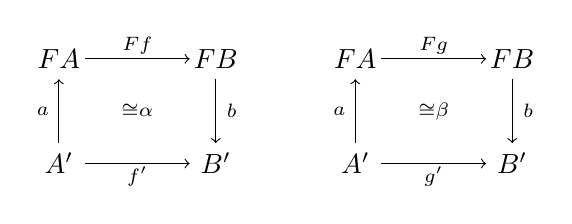
\begin{tikzpicture}[x=1.05em,y=1.05em]
    \node at (0,2.2)    {$FA$};
    \node at (5.4,2.2)  {$FB$};
    \node at (0,-1.4)   {$A'$};
    \node at (5.4,-1.4) {$B'$};
    \draw[->] (0.9,2.2) -- (4.5,2.2);
    \node at (2.7,2.66) {$\scriptstyle Ff$};
    \draw[->] (0,-0.7) -- (0,1.5);
    \node at (-0.55,0.4) {$\scriptstyle a$};
    \draw[->] (5.4,1.5) -- (5.4,-0.7);
    \node at (5.95,0.4) {$\scriptstyle b$};
    \draw[->] (0.9,-1.4) -- (4.5,-1.4);
    \node at (2.7,-1.86) {$\scriptstyle f'$};
    \node at (2.7,0.4) {$\scriptstyle\cong\alpha$};
    \begin{scope}[shift={(10.2,0)}]
      \node at (0,2.2)    {$FA$};
      \node at (5.4,2.2)  {$FB$};
      \node at (0,-1.4)   {$A'$};
      \node at (5.4,-1.4) {$B'$};
      \draw[->] (0.9,2.2) -- (4.5,2.2);
      \node at (2.7,2.66) {$\scriptstyle Fg$};
      \draw[->] (0,-0.7) -- (0,1.5);
      \node at (-0.55,0.4) {$\scriptstyle a$};
      \draw[->] (5.4,1.5) -- (5.4,-0.7);
      \node at (5.95,0.4) {$\scriptstyle b$};
      \draw[->] (0.9,-1.4) -- (4.5,-1.4);
      \node at (2.7,-1.86) {$\scriptstyle g'$};
      \node at (2.7,0.4) {$\scriptstyle\cong\beta$};
    \end{scope}
  \end{tikzpicture}
  \end{center}
  则映射 \eqref{eq:homotopy-categories-map} 在 $\mathcal{K}$ 中诸%
  \trNaturalTransformation{} $f\Rightarrow g$ 与 $\mathcal{L}$ 中诸%
  \trNaturalTransformation{} $f'\Rightarrow g'$ 之间诱导一个双射。
\end{enumerate}
\end{corollary}

\begin{proof}
\cref{lem:biequivalence-reflect-create}证明了\trCosmologicalBiequivalence{}保持、反射并创造诸\trEquivalence，其论证根本上是 2-\trCategory{}式的，请读者重访之。这一点连同\trCosmologicalBiequivalence{}的本质满性，蕴含此类\trFunctor{}在对象的\trEquivalence{}类上诱导一个双射。这就证明了 (i)。

至于 (ii)，由\cref{cor:functor-space-equivalences}，所选的\trEquivalence
$FA\simeq A'$ 与 $FB\simeq B'$ 诱导诸%
\trQuasiCategory{}之间的一个\trEquivalence
\begin{equation*}
\Fun(A,B)\xrightarrow{\ \sim\ }\Fun(FA,FB)\xrightarrow{\ \sim\ }\Fun(A',B')
\end{equation*}
它下降为诸\trHomotopyCategory{}的\trEquivalence{} \eqref{eq:homotopy-categories-map}。由于诸\trQuasiCategory{}之间的\trEquivalence{}在顶点的\trIsomorphism{}类之间诱导双射，这特别地给出诸\trFunctor{}的\trIsomorphism{}类之间的一个双射。

至于 (iii)，\trEquivalence{} \eqref{eq:homotopy-categories-map} 是\trFullyFaithful，在诸\trNaturalTransformation{} $f\Rightarrow g$ 与
$b\cdot Ff\cdot a\Rightarrow b\cdot Fg\cdot a$ 之间诱导一个双射。这一双射可沿任何所选的\trIsomorphism{} $\alpha$ 与 $\beta$ 搬运，给出 $\mathcal{K}$ 中 $\hFun(A,B)$ 内诸\trNaturalTransformation{} $f\Rightarrow g$ 与 $\mathcal{L}$ 中 $\hFun(A',B')$ 内诸\trNaturalTransformation{} $f'\Rightarrow g'$ 之间的一个双射。
\end{proof}

作为\cref{cor:biequivalence-local-bijections}的一个应用，我们现在兑现 2.3 节所作的一个承诺：确立 $(\infty,1)$-\trCategory{}的\trInfinityCosmos{}中%
\trInfinityCategory{} $A$ 与 $B$ 之间的\trInternalHom{} $B^{A}$，同 $B$ 与 $A$ 的\trUnderlyingQuasiCategory{}的单纯\trCotensor{} $B^{A_{0}}$ 之间的一个\trEquivalence。

\begin{observation}\label{obs:weak-exponentials}
即使 $(\infty,1)$-\trCategory{}的一个\trInfinityCosmos{} $\mathcal{K}$ 不是\trCartesianClosed，其\trHomotopyTwoCategory{} $\mathfrak{h}\mathcal{K}$ 在\trBicategorical{}意义下也是\trCartesianClosed——以自然\trEquivalence{}替换\cref{prop:cartesian-closure}(ii) 的诸自然\trIsomorphism。由于\cref{prop:underlying-qcat-biequivalence}的\trBiequivalence{} $(-)_{0}\colon\mathcal{K}\Rightarrow\QCat$，我们定义 $B^{A}\in\mathcal{K}$ 为任一\trUnderlyingQuasiCategory{}等价于 $B_{0}^{A_{0}}$ 的\trInfinityCategory。经由复合诸\trEquivalence
\begin{center}
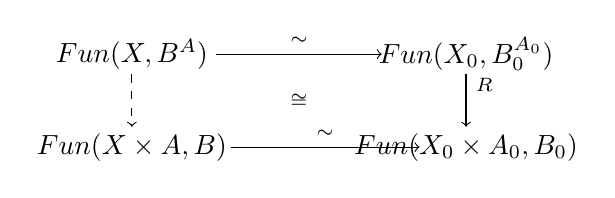
\begin{tikzpicture}[x=1.05em,y=1.05em]
  \node (a) at (0,0)    {$\Fun(X,B^{A})$};
  \node (b) at (11.5,0) {$\Fun(X_{0},B_{0}^{A_{0}})$};
  \node (c) at (0,-3.2) {$\Fun(X\times A,B)$};
  \node (d) at (11.5,-3.2) {$\Fun(X_{0}\times A_{0},B_{0})$};
  \draw[->] (2.9,0) -- node[above]{$\scriptstyle\sim$} (8.6,0);
  \draw[->] (3.4,-3.2) -- node[above]{$\scriptstyle\sim$} (9.9,-3.2);
  \draw[->,dashed] (0,-0.7) -- (0,-2.5);
  \draw[->] (11.5,-0.7) -- node[right,pos=0.2]{$\scriptstyle R$} (11.5,-2.5);
  \node at (5.75,-1.6) {$\scriptstyle\cong$};
\end{tikzpicture}
\end{center}
我们见到：对任何 $X$，$\Fun(X,B^{A})\simeq\Fun(X\times A,B)$。在定义 10.4.13
的术语中，映射 $\Fun(X,B^{A})\Rightarrow\Fun(X\times A,B)$ 是一个%
\emph{拟伪自然等价}（quasi-pseudonatural equivalence）。注意，若 $\mathcal{K}$ 是\trCartesianClosed，这一\trUniversalProperty{}表明诸弱指数等价于严格定义者。
\end{observation}

出于这一理由，\cref{prop:exponential-cotensor}的陈述不要求环境%
\trInfinityCosmos{}是\trCartesianClosed；诸指数可以事后推得存在。

\begin{proposition}\label{prop:exponential-cotensor}
在 $(\infty,1)$-\trCategory{}的一个\trInfinityCosmos{}中，对任何%
\trInfinityCategory{} $A$ 与 $B$，指数 $B^{A}$ 等价于 $B$ 与 $A$ 的\trUnderlyingQuasiCategory{}的\trCotensor{} $B^{A_{0}}$。
\end{proposition}

\begin{proof}
由\cref{cor:biequivalence-local-bijections}，诸\trCosmologicalBiequivalence{}反射诸\trInfinityCategory{}之间的\trEquivalence。于是，为证
$B^{A}\simeq B^{A_{0}}$，由\cref{prop:underlying-qcat-biequivalence}与%
\cref{cor:biequivalence-local-bijections}，只需证明 $B^{A}$ 与 $B^{A_{0}}$ 具有等价的\trUnderlyingQuasiCategory。指数与\trCotensor{}的定义性\trUniversalProperty{}提供诸\trEquivalence，它们与\trUnderlyingQuasiCategory{}函子的\trLocalEquivalence{}复合，给出所要的\trEquivalence：
\begin{equation*}
\Fun(1,B^{A})\simeq\Fun(A,B)\xrightarrow{\ \sim\ }\Fun(A_{0},B_{0})\simeq\Fun(1,B^{A_{0}})
\end{equation*}
\end{proof}

我们现在证明：\trBiequivalence{}对于\cref{prop:cosmological-preservation-properties}所考虑的诸∞-范畴论结构，在保持之外还反射并创造它们。

\begin{proposition}\label{prop:biequivalence-reflects-creates}
一个\trCosmologicalBiequivalence{} $F\colon\mathcal{K}\Rightarrow\mathcal{L}$
\begin{enumerate}[label=(\roman*)]
\item 保持、反射并创造诸\trEquivalence。
\item 保持并反射诸\trNaturalTransformation{}的可逆性，并在给定的诸\trFunctor{}之间创造诸自然\trIsomorphism。
\item 保持、反射并创造诸\trInfinityCategory{}之间的\trAdjunction，包括右伴随右逆伴随与左伴随右逆伴随。
\item 保持、反射并创造\trFiberedAdjunction{}与\trFiberedEquivalence。
\item 保持并反射离散性。
\item 保持并反射\trCommaInfinityCategory：一个\trCell{}定义 $\mathcal{K}$ 中的一个\trCommaCone，当且仅当它的像是 $\mathcal{L}$ 中的一个\trCommaCone。
\item 保持、反射并创造给定\trCospan{}之上的\trAbsoluteRightLifting{}图表与\trAbsoluteLeftLifting{}图表。
\item 保持并反射以\trSimplicialSet{}为指标的\trDiagram{}之\trLimit{}或\trColimit，并创造「一个\trInfinityCategory{}容许给定\trDiagram{}之\trLimit{}或\trColimit」这一性质。
\item 保持并反射一个\trInfinityCategory{}的稳定性与此类\trInfinityCategory{}之间的诸\trFunctor{}的正合性。
\item 保持并反射\trCartesianFibration{}与\trCocartesianFibration{}及其间的\trCartesianFunctor。
\item 保持并反射\trDiscreteCartesianFibration{}与\trDiscreteCocartesianFibration。
\item 保持并反射\trTwoSidedFibration{}及其间的\trCartesianFunctor。
\item 保持并反射\trModule{}与可表示模，并对一对固定的\trInfinityCategory{}之间的诸\trModule{}之\trEquivalence{}类诱导一个双射。
\end{enumerate}
\end{proposition}

\begin{proof}
诸保持性质已在\cref{prop:cosmological-preservation-properties}中、于较弱的假设——$F$ 只是一个\trCosmologicalFunctor——之下获证。于是只剩下处理诸性质的反射与诸∞-范畴论结构的创造。

性质 (i)、(ii) 与 (iii) 对 2-范畴之间的任何\trBiequivalence{}都成立——例如 $F\colon\mathfrak{h}\mathcal{K}\Rightarrow\mathfrak{h}\mathcal{L}$。尚未论及的那些方面留给\cref{ex:two-categorical-biequivalence}——这是一道有益的练习，可藉之熟悉双等价的 2-\trCategory{}式概念。由\cref{prop:slice-biequivalence}，(iv) 是 (i) 与 (iii) 的特例。

性质 (v) 由 (ii) 得出：若 $FE$ 是\trDiscrete，则 $\mathcal{K}$ 中任何以 $E$ 为余定义域的 2-\trCell{}在 $F$ 之下的像是可逆的，这就蕴含该 2-\trCell{}在 $E$ 中是\trInvertible。

由于 $\mathcal{K}$ 与 $\mathcal{L}$ 二者都容许\trCommaInfinityCategory，而命题 3.4.11 表明诸\trCommaSpan{}由\trTwoSidedIsofibration{}的一个\trFiberedEquivalence{}类所刻画，故 (vi) 由 (iv) 得出。

(vii) 与 (viii) 的反射性质由定理 3.5.3 得出，而创造性质由定理 3.5.12 与 (vi) 得出。然后，(ix) 可借定理 4.4.12 中任何一组等价刻画、利用 (ii) 与 (viii) 得到论证。

条目 (x) 经由定理 5.2.8 由 (iii) 与 (ii) 得出，而 (xi) 由把 (i) 应用于命题 5.5.8 所考虑的那个态射得出。性质 (xii) 类似地由定理 7.1.4(iii) 以及 (iii) 与 (ii) 得出。\trModule{}的保持与反射现在由这一点与 (v) 得出，而\trEquivalence{}类之间的双射由 (iv) 得出。\footnote{更精确的陈述出现于命题 11.1.4。}(xiii) 的可表示性陈述把 (iv) 与 (vi) 相结合，如命题 11.1.5 所详论。
\end{proof}

\begin{corollary}\label{cor:induced-biequivalences}
若 $F\colon\mathcal{K}\Rightarrow\mathcal{L}$ 是一个\trCosmologicalBiequivalence，则下列受诱导的\trCosmologicalFunctor{}都是\trBiequivalence：
\begin{enumerate}[label=(\roman*)]
\item $F\colon\Disc(\mathcal{K})\Rightarrow\Disc(\mathcal{L})$
\item $F\colon\mathcal{K}_{\top,J}\Rightarrow\mathcal{L}_{\top,J}$
  与 $F\colon\mathcal{K}_{\bot,J}\Rightarrow\mathcal{L}_{\bot,J}$
\item $F\colon\Rari(\mathcal{K})_{/B}\Rightarrow\Rari(\mathcal{L})_{/FB}$
  与 $F\colon\Lari(\mathcal{K})_{/B}\Rightarrow\Lari(\mathcal{L})_{/FB}$
\item $F\colon\Rari(\mathcal{K})\Rightarrow\Rari(\mathcal{L})$
  与 $F\colon\Lari(\mathcal{K})\Rightarrow\Lari(\mathcal{L})$
\item $F\colon\Cart(\mathcal{K})_{/B}\Rightarrow\Cart(\mathcal{L})_{/FB}$
  与 $F\colon\CoCart(\mathcal{K})_{/B}\Rightarrow\CoCart(\mathcal{L})_{/FB}$
\item $F\colon\Cart(\mathcal{K})\Rightarrow\Cart(\mathcal{L})$
  与 $F\colon\CoCart(\mathcal{K})\Rightarrow\CoCart(\mathcal{L})$
\item $F\colon\Disc\Cart(\mathcal{K})\Rightarrow\Disc\Cart(\mathcal{L})$
  与 $F\colon\Disc\CoCart(\mathcal{K})\Rightarrow\Disc\CoCart(\mathcal{L})$
\item $F\colon\Stab(\mathcal{K})\Rightarrow\Stab(\mathcal{L})$
\item $F\colon{}_{A}\Fib(\mathcal{K})_{/B}\Rightarrow{}_{FA}\Fib(\mathcal{L})_{/FB}$
\item $F\colon{}_{A}\Mod(\mathcal{K})_{/B}\Rightarrow{}_{FA}\Mod(\mathcal{L})_{/FB}$
\end{enumerate}
\end{corollary}

\begin{proof}
在每一种情形，我们都从一个\trCosmologicalBiequivalence{}出发——例如
$\mathcal{K}_{/B}\Rightarrow\mathcal{L}_{/FB}$ 或
$\mathcal{K}^{\dagger}\Rightarrow\mathcal{L}^{\dagger}$——而必须证明：%
\cref{lem:restrict-replete-cosmological}限制所得的\trCosmologicalFunctor{}仍然是诸\trCosmologicallyEmbedded{}\trInfinityCosmos{}之间的一个\trBiequivalence。每一个论证都是类似的；为具体起见，我们证明 (viii)。\cref{prop:biequivalence-reflects-creates}证明了：刻画该子\trInfinityCosmos{}的对象与 0-箭头的那种性质为任何\trBiequivalence{}所保持并反射。于是，诸\trCosmologicalFunctor{}的图表是一个\trPullback：
\begin{center}
\begin{tikzpicture}[x=1.05em,y=1.05em]
  \node at (0,1.7)    {$\Stab(\mathcal{K})$};
  \node at (8.2,1.7)  {$\Stab(\mathcal{L})$};
  \node at (0,-1.7)   {$\mathcal{K}$};
  \node at (8.2,-1.7) {$\mathcal{L}$};
  \draw[->] (2.9,1.7) -- (5.3,1.7);
  \node at (4.1,2.14) {$\scriptstyle F$};
  \draw[right hook->] (0,1.1) -- (0,-1.1);
  \draw[right hook->] (8.2,1.1) -- (8.2,-1.1);
  \draw[->] (2.2,-1.7) -- (6.0,-1.7);
  \node at (4.1,-1.26) {$\scriptstyle\sim$};
  \node at (4.1,-2.16) {$\scriptstyle F$};
  \node at (1.55,1.05) {$\scriptstyle\lrcorner$};
\end{tikzpicture}
\end{center}
故\cref{lem:pullback-cosmological-biequivalence}容许我们断言：受诱导的\trFunctor{} $\Stab(\mathcal{K})\Rightarrow\Stab(\mathcal{L})$ 是一个\trCosmologicalBiequivalence。
\end{proof}

\cref{war:composites-not-preserved}提到过一些未必为\trCosmologicalFunctor{}所保持的∞-范畴论性质。重要的是，这些概念为\trCosmologicalBiequivalence{}所保持、反射并创造。引理 11.1.7 就复合与\trExactSquare{}这两种情形证明了这一点——这两个概念居于模的\trVirtualEquipment{}之中——而我们现在处理逐点右\trExtension{}与逐点左\trExtension{}的情形。

\begin{proposition}\label{prop:pointwise-extensions-biequivalence}
一个\trCosmologicalBiequivalence{} $F\colon\mathcal{K}\Rightarrow\mathcal{L}$
保持、反射并创造逐点左\trExtension{}与逐点右\trExtension：
\begin{enumerate}[label=(\roman*)]
\item $\mathcal{K}$ 中如下形式的\trDiagram
\begin{center}
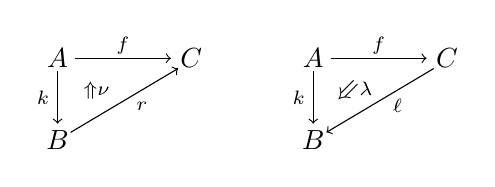
\begin{tikzpicture}[x=1.05em,y=1.05em]
  \node at (0,2.2)   {$A$};
  \node at (4.6,2.2) {$C$};
  \node at (0,-0.6)  {$B$};
  \draw[->] (0.6,2.2) -- (3.9,2.2);
  \node at (2.25,2.64) {$\scriptstyle f$};
  \draw[->] (0,1.75) -- (0,-0.05);
  \node at (-0.5,0.85) {$\scriptstyle k$};
  \draw[->] (0.45,-0.35) -- (4.15,1.85);
  \node at (2.9,0.55) {$\scriptstyle r$};
  \node at (1.35,1.1) {$\scriptstyle\Uparrow\nu$};
  \begin{scope}[shift={(8.8,0)}]
    \node at (0,2.2)   {$A$};
    \node at (4.6,2.2) {$C$};
    \node at (0,-0.6)  {$B$};
    \draw[->] (0.6,2.2) -- (3.9,2.2);
    \node at (2.25,2.64) {$\scriptstyle f$};
    \draw[->] (0,1.75) -- (0,-0.05);
    \node at (-0.5,0.85) {$\scriptstyle k$};
    \draw[->] (4.15,1.85) -- (0.45,-0.35);
    \node at (2.9,0.55) {$\scriptstyle\ell$};
    \node at (1.35,1.1) {$\scriptstyle\SWarrow\lambda$};
  \end{scope}
\end{tikzpicture}
\end{center}
定义 $\mathcal{K}$ 中的一个逐点右\trExtension{}或逐点左\trExtension，当且仅当其在 $F$ 之下的像分别定义 $\mathcal{L}$ 中的一个逐点右\trExtension{}或逐点左\trExtension。
\item 若 $\mathcal{K}$ 中的诸\trFunctor{} $f\colon A\to C$ 与 $k\colon A\to B$ 使得 $Ff\colon FA\to FC$ 在 $\mathcal{L}$ 中沿 $Fk\colon FA\to FB$ 容许一个逐点右\trExtension{}或逐点左\trExtension，则 $f$ 在 $\mathcal{K}$ 中分别沿 $k$ 容许一个逐点右\trExtension{}或逐点左\trExtension，且其在 $F$ 之下的像同构于 $\mathcal{L}$ 中的相应数据。
\end{enumerate}
\end{proposition}

为解释证明的想法，我们首先证明\trCosmologicalBiequivalence{}保持并反射右\trExtension；它们也创造右\trExtension，但这在逐点情形可以同样容易地证明，逐点情形随后讨论。

首先设 $\nu\colon rk\Rightarrow f$ 是 $\mathcal{K}$ 中的一个右\trExtension。为证其像定义 $\mathcal{L}$ 中的一个右\trExtension，我们必须证明：对所有 $d\colon FB\to FC$，映射
\begin{equation*}
\begin{gathered}
\hFun(FB,FC)(d,Fr)\xrightarrow{\ F\nu\circ\ }\hFun(FA,FC)(d\cdot Fk,Ff)\\
d\overset{\gamma}{\Rightarrow}Fr\longmapsto d\cdot Fk\overset{\gamma Fk}{\Rightarrow}Fr\cdot Fk\overset{F\nu}{\Rightarrow}Ff
\end{gathered}
\end{equation*}
在诸 2-\trCell{}的集合上定义一个双射。由\cref{cor:biequivalence-local-bijections}(ii)，存在 $\mathcal{K}$ 中一个\trFunctor{} $c\colon B\to C$ 连同一个自然\trIsomorphism{} $\delta\colon d\cong Fc$。由\cref{cor:biequivalence-local-bijections}(iii)，$F$ 的应用与同 $\delta$ 的复合定义一个双射
\begin{equation*}
\begin{gathered}
\hFun(B,C)(c,r)\xrightarrow{\ F\ }\hFun(FB,FC)(Fc,Fr)\xrightarrow{\ -\circ\delta\ }\hFun(FB,FC)(d,Fr)\\
c\overset{\alpha}{\Rightarrow}r\longmapsto Fc\overset{F\alpha}{\Rightarrow}Fr\longmapsto d\overset{\delta}{\Rightarrow}Fc\overset{F\alpha}{\Rightarrow}Fr
\end{gathered}
\end{equation*}
从可逆 2-\trCell{} $\delta Fk\colon d\cdot Fk\cong Fc\cdot Fk$ 出发可定义一个类似的双射。由于 $\nu\colon rk\Rightarrow f$ 是一个右\trExtension，与 $\nu$ 的复合诱导出它自己的一族双射。从函数的如下交换方块——其中三个已知为双射——我们见到：$F\nu\colon Fr\cdot Fk\Rightarrow Ff$ 是 $\mathcal{L}$ 中的一个右\trExtension，如所断言。
\begin{center}
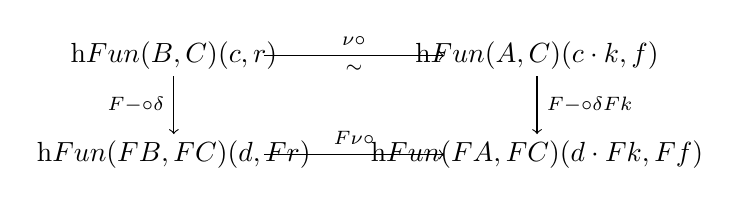
\begin{tikzpicture}[x=1.05em,y=1.05em]
  \node (a) at (0,0)     {$\hFun(B,C)(c,r)$};
  \node (b) at (12.5,0)  {$\hFun(A,C)(c\cdot k,f)$};
  \node (c) at (0,-3.4)  {$\hFun(FB,FC)(d,Fr)$};
  \node (d) at (12.5,-3.4) {$\hFun(FA,FC)(d\cdot Fk,Ff)$};
  \draw[->] (3.1,0) -- node[above]{$\scriptstyle\nu\circ$} node[below]{$\scriptstyle\sim$} (9.3,0);
  \draw[->] (0,-0.7) -- node[left]{$\scriptstyle F-\circ\delta$} (0,-2.7);
  \draw[->] (12.5,-0.7) -- node[right]{$\scriptstyle F-\circ\delta Fk$} (12.5,-2.7);
  \draw[->] (3.1,-3.4) -- node[above]{$\scriptstyle F\nu\circ$} (9.3,-3.4);
\end{tikzpicture}
\end{center}

现在设 $F\nu\colon Fr\cdot Fk\Rightarrow Ff$ 是 $\mathcal{L}$ 中的一个右\trExtension。为见 $\nu\colon rk\Rightarrow f$ 是 $\mathcal{K}$ 中的一个右\trExtension，注意对任何\trFunctor{} $c\colon B\to C$，有函数的如下交换方块
\begin{center}
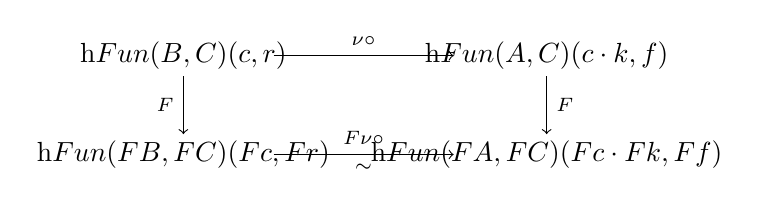
\begin{tikzpicture}[x=1.05em,y=1.05em]
  \node (a) at (0,0)     {$\hFun(B,C)(c,r)$};
  \node (b) at (12.5,0)  {$\hFun(A,C)(c\cdot k,f)$};
  \node (c) at (0,-3.4)  {$\hFun(FB,FC)(Fc,Fr)$};
  \node (d) at (12.5,-3.4) {$\hFun(FA,FC)(Fc\cdot Fk,Ff)$};
  \draw[->] (3.1,0) -- node[above]{$\scriptstyle\nu\circ$} (9.3,0);
  \draw[->] (0,-0.7) -- node[left]{$\scriptstyle F$} (0,-2.7);
  \draw[->] (12.5,-0.7) -- node[right]{$\scriptstyle F$} (12.5,-2.7);
  \draw[->] (3.1,-3.4) -- node[above]{$\scriptstyle F\nu\circ$} node[below]{$\scriptstyle\sim$} (9.3,-3.4);
\end{tikzpicture}
\end{center}
其中三个已知为双射。这就证明了 $\nu\colon rk\Rightarrow f$ 具有右\trExtension{}的\trUniversalProperty。

逐点右\trExtension{}的论证本质相同，其中我们额外利用「\trCommaInfinityCategory{}为\trCosmologicalFunctor{}所保持且在\trEquivalence{}之下不变」这一事实（练习 3.4.iv 之义）。

\begin{proof}
我们全程使用\cref{thm:pointwise-right-extensions}(ii) 所给的逐点右\trExtension{}的 2-范畴式定义。想法是利用\cref{cor:biequivalence-local-bijections}所提供的诸局部双射。

设 $\nu\colon rk\Rightarrow f$ 是 $\mathcal{K}$ 中的一个逐点右\trExtension。我们必须证明：对 $\mathcal{L}$ 中每个 $h\colon L\to FB$，图表
\begin{center}
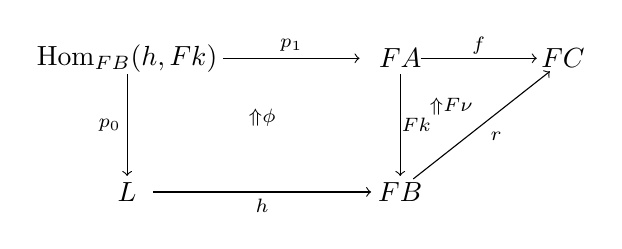
\begin{tikzpicture}[x=1.05em,y=1.05em]
  \node at (0,2.6)    {$\HomFB(h,Fk)$};
  \node at (9.4,2.6)  {$FA$};
  \node at (15.0,2.6) {$FC$};
  \node at (0,-2.0)   {$L$};
  \node at (9.4,-2.0) {$FB$};
  \draw[->] (3.3,2.6) -- (8.0,2.6);
  \node at (5.65,3.04) {$\scriptstyle p_{1}$};
  \draw[->] (10.1,2.6) -- (14.1,2.6);
  \node at (12.1,3.04) {$\scriptstyle f$};
  \draw[->] (0,2.05) -- (0,-1.45);
  \node at (-0.6,0.3) {$\scriptstyle p_{0}$};
  \draw[->] (9.4,2.05) -- (9.4,-1.45);
  \node at (9.95,0.3) {$\scriptstyle Fk$};
  \draw[->] (0.9,-2.0) -- (8.4,-2.0);
  \node at (4.65,-2.46) {$\scriptstyle h$};
  \draw[->] (9.85,-1.55) -- (14.55,2.15);
  \node at (12.7,-0.1) {$\scriptstyle r$};
  \node at (4.65,0.55) {$\scriptstyle\Uparrow\phi$};
  \node at (11.15,0.95) {$\scriptstyle\Uparrow F\nu$};
\end{tikzpicture}
\end{center}
是 $\mathcal{L}$ 中的一个右\trExtension{}图表，也就是说：对所有 $d\colon L\to FC$\footnote{原书印作「$d\colon L\Rightarrow FC$」（双杆），而 p.400 同语境印作「$d\colon FB\to FC$」（单杆），前后摇摆不一，此处按 0-箭头记号体系统一作单杆。——译者注}，映射
\begin{equation*}
\begin{gathered}
\hFun(L,FC)(d,Fr\cdot h)\xrightarrow{\ F\nu p_{1}\circ F\phi\circ\ }\hFun(\HomFB(h,Fk))(dp_{0},Ff\cdot p_{1})\\
d\overset{\varsigma}{\Rightarrow}Fr\cdot h\longmapsto dp_{0}\overset{\varsigma p_{0}}{\Rightarrow}Fr\cdot hp_{0}\overset{Fr\phi}{\Rightarrow}Fr\cdot Fk\cdot p_{1}\overset{F\nu p_{1}}{\Rightarrow}Ff\cdot p_{1}
\end{gathered}
\end{equation*}
定义诸 2-\trCell{}集合之间的一个双射。由\cref{cor:biequivalence-local-bijections}(i)，存在一个\trInfinityCategory{} $K\in\mathcal{K}$ 与一支\trEquivalence{} $e\colon L\Rightarrow FK$；由\cref{cor:biequivalence-local-bijections}(ii)，存在诸\trFunctor{} $b\colon K\to B$ 与 $c\colon K\to C$ 以及自然\trIsomorphism{} $\beta\colon Fb\cdot e\cong h$ 与 $\delta\colon d\cong Fc\cdot e$。由\cref{cor:biequivalence-local-bijections}(iii)，$F$ 的应用与同 $e$、$\beta$、$\delta$ 的复合定义一个双射\footnote{原书此双射式右端印作「$\Fun(L,FC)(d,Fr\cdot h)$」，缺同伦范畴函子之字头（同式左端实印「$\hFun(K,C)(c,rb)$」，带 $\mathrm{h}$）；按上下文此式诸项皆为同伦范畴间之态射，应为 $\hFun(L,FC)(d,Fr\cdot h)$ 之漏排，此处径补。——译者注}
\begin{equation*}
\begin{gathered}
\hFun(K,C)(c,rb)\xrightarrow{\ \sim\ }\hFun(L,FC)(d,Fr\cdot h)\\
c\overset{\gamma}{\Rightarrow}rb\longmapsto d\overset{\delta}{\Rightarrow}Fc\cdot e\overset{F\gamma e}{\Rightarrow}Fr\cdot Fb\cdot e\overset{Fr\beta}{\Rightarrow}Fr\cdot h
\end{gathered}
\end{equation*}

由于 $\nu\colon rk\Rightarrow f$ 是 $\mathcal{K}$ 中的一个逐点右\trExtension，图表
\begin{rveq}\label{eq:pointwise-right-extension-diagram}
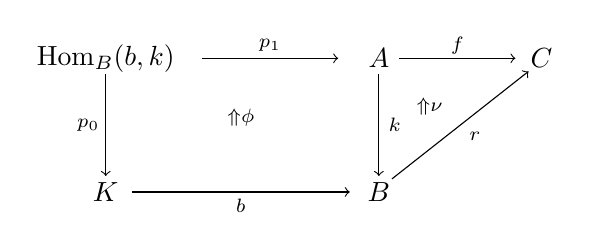
\begin{tikzpicture}[x=1.05em,y=1.05em]
  \node at (0,2.6)    {$\HomB(b,k)$};
  \node at (9.4,2.6)  {$A$};
  \node at (15.0,2.6) {$C$};
  \node at (0,-2.0)   {$K$};
  \node at (9.4,-2.0) {$B$};
  \draw[->] (3.3,2.6) -- (8.0,2.6);
  \node at (5.65,3.04) {$\scriptstyle p_{1}$};
  \draw[->] (10.1,2.6) -- (14.1,2.6);
  \node at (12.1,3.04) {$\scriptstyle f$};
  \draw[->] (0,2.05) -- (0,-1.45);
  \node at (-0.6,0.3) {$\scriptstyle p_{0}$};
  \draw[->] (9.4,2.05) -- (9.4,-1.45);
  \node at (9.95,0.3) {$\scriptstyle k$};
  \draw[->] (0.9,-2.0) -- (8.4,-2.0);
  \node at (4.65,-2.46) {$\scriptstyle b$};
  \draw[->] (9.85,-1.55) -- (14.55,2.15);
  \node at (12.7,-0.1) {$\scriptstyle r$};
  \node at (4.65,0.55) {$\scriptstyle\Uparrow\phi$};
  \node at (11.15,0.95) {$\scriptstyle\Uparrow\nu$};
\end{tikzpicture}
\end{rveq}
也是一个（逐点）右\trExtension，定义出双射
\begin{equation*}
\begin{gathered}
\hFun(K,C)(c,rb)\xrightarrow{\ \simeq\ }\hFun(\HomB(b,k),C)(cp_{0},fp_{1})\\
c\overset{\gamma}{\Rightarrow}rb\longmapsto cp_{0}\overset{\gamma p_{0}}{\Rightarrow}rbp_{0}\overset{r\phi}{\Rightarrow}rkp_{1}\overset{\nu p_{1}}{\Rightarrow}fp_{1}
\end{gathered}
\end{equation*}

由练习 3.4.iv 有一个等价\hspace{-1pt}$y\colon\HomFB(h,Fk)\Rightarrow\HomFB(Fb,Fk)\cong Fb\,\HomB(b,k)$ 居于 $e\times\mathrm{id}\colon L\times FA\Rightarrow FK\times FA$ 之上。
由\cref{cor:biequivalence-local-bijections}(iii)，$F$ 的应用与同 $y$、$\beta$、$\delta$ 的复合定义出函数的如下交换方块中右侧的那个双射
\begin{center}
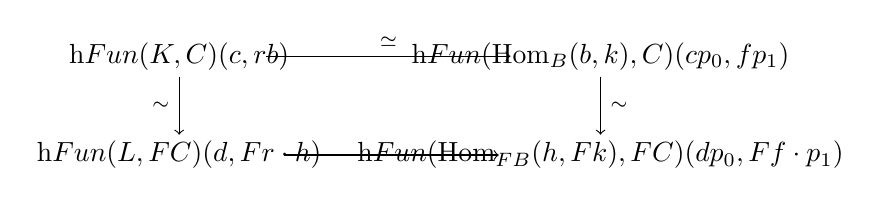
\begin{tikzpicture}[x=1.05em,y=1.05em]
  \node (a) at (0,0)     {$\hFun(K,C)(c,rb)$};
  \node (b) at (14.5,0)  {$\hFun(\HomB(b,k),C)(cp_{0},fp_{1})$};
  \node (c) at (0,-3.4)  {$\hFun(L,FC)(d,Fr\cdot h)$};
  \node (d) at (14.5,-3.4) {$\hFun(\HomFB(h,Fk),FC)(dp_{0},Ff\cdot p_{1})$};
  \draw[->] (3.0,0) -- node[above]{$\scriptstyle\simeq$} (11.4,0);
  \draw[->] (0,-0.7) -- node[left]{$\scriptstyle\sim$} (0,-2.7);
  \draw[->] (14.5,-0.7) -- node[right]{$\scriptstyle\sim$} (14.5,-2.7);
  \draw[->] (3.6,-3.4) -- (11.0,-3.4);
\end{tikzpicture}
\end{center}
于是 $\mathcal{L}$ 中我们的粘贴图表是一个右\trExtension{}图表，如所欲证。

为见逐点右\trExtension{}被反射，我们必须在「$F\nu\colon Fr\cdot Fk\Rightarrow Ff$ 是 $\mathcal{L}$ 中一个逐点右\trExtension{}图表」这一假设之下证明：\eqref{eq:pointwise-right-extension-diagram} 是 $\mathcal{K}$ 中的一个右\trExtension{}图表。对任何\trFunctor{} $c\colon K\to C$，有函数的如下交换方块：
\begin{center}
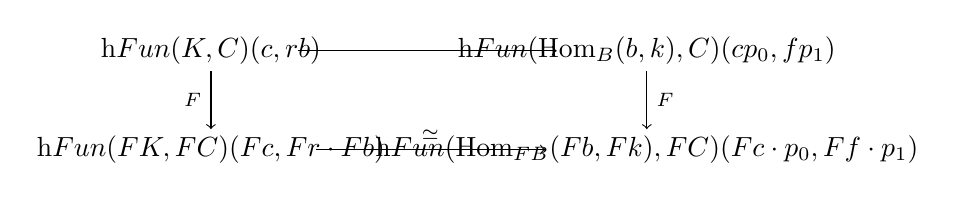
\begin{tikzpicture}[x=1.05em,y=1.05em]
  \node (a) at (0,0)     {$\hFun(K,C)(c,rb)$};
  \node (b) at (15.0,0)  {$\hFun(\HomB(b,k),C)(cp_{0},fp_{1})$};
  \node (c) at (0,-3.4)  {$\hFun(FK,FC)(Fc,Fr\cdot Fb)$};
  \node (d) at (15.0,-3.4) {$\hFun(\HomFB(Fb,Fk),FC)(Fc\cdot p_{0},Ff\cdot p_{1})$};
  \draw[->] (3.0,0) -- (11.9,0);
  \draw[->] (0,-0.7) -- node[left]{$\scriptstyle F$} (0,-2.7);
  \draw[->] (15.0,-0.7) -- node[right]{$\scriptstyle F$} (15.0,-2.7);
  \draw[->] (3.6,-3.4) -- node[above]{$\scriptstyle\simeq$} (11.5,-3.4);
\end{tikzpicture}
\end{center}
由于\trCommaSquare{}为\trCosmologicalFunctor{}所保持，底部映射是一个双射——由 $F$ 的应用所定义的诸竖直函数亦然。于是，$\nu\colon r\cdot k\Rightarrow f$ 满足 $\mathcal{K}$ 中逐点右\trExtension{}的\trUniversalProperty。

最后，为见逐点右\trExtension{}图表为\trCosmologicalBiequivalence{}所创造，设给定 $\mathcal{L}$ 中一个逐点右\trExtension{}图表
\begin{center}
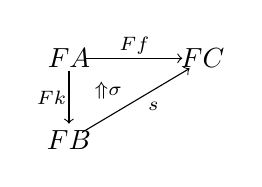
\begin{tikzpicture}[x=1.05em,y=1.05em]
  \node at (0,2.2)   {$FA$};
  \node at (4.6,2.2) {$FC$};
  \node at (0,-0.6)  {$FB$};
  \draw[->] (0.6,2.2) -- (3.9,2.2);
  \node at (2.25,2.64) {$\scriptstyle Ff$};
  \draw[->] (0,1.75) -- (0,-0.05);
  \node at (-0.6,0.85) {$\scriptstyle Fk$};
  \draw[->] (0.45,-0.35) -- (4.15,1.85);
  \node at (2.9,0.55) {$\scriptstyle s$};
  \node at (1.35,1.1) {$\scriptstyle\Uparrow\sigma$};
\end{tikzpicture}
\end{center}
由\cref{cor:biequivalence-local-bijections}，存在一个\trFunctor{} $r\colon B\to C$ 连同\trIsomorphism{} $\alpha\colon s\cong Fr$ 与一支\trNaturalTransformation{} $\nu\colon rk\Rightarrow f$，后者在双射
\begin{equation*}
\begin{gathered}
\hFun(A,C)(rk,f)\xrightarrow{\ F(-)\circ\alpha Fk\ }\hFun(FA,FC)(s\cdot Fk,Ff)\\
rk\overset{\nu}{\Rightarrow}f\longmapsto s\cdot Fk\overset{\sigma}{\Rightarrow}Ff
\end{gathered}
\end{equation*}
之下被映射为 $\sigma$。由于 $F\nu$ 同构于 $\mathcal{L}$ 中一个逐点右\trExtension{}图表，它是 $\mathcal{L}$ 中一个逐点右\trExtension{}图表；而由于逐点右\trExtension{}图表为\trCosmologicalBiequivalence{}所反射，$\nu$ 展示 $r$ 为 $f$ 沿 $k$ 的一个逐点右\trExtension，如所断言。
\end{proof}

立即得自定义 9.4.7 与引理 9.5.6：
\begin{corollary}\label{cor:weighted-limits-biequivalence}
\trCosmologicalBiequivalence{}保持、反射并创造以\trInfinityCategory{}为指标的\trDiagram{}之（加权）\trLimit{}与\trColimit。\qed
\end{corollary}

\subsection*{练习}

\begin{exercise}\label{ex:homotopy-category-change-of-model}
设 $F\colon\mathcal{K}\Rightarrow\mathcal{L}$ 是一个\trCosmologicalBiequivalence。请证明：$F$ 对任何\trInfinityCategory{} $A\in\mathcal{K}$ 都诱导诸\trHomotopyCategory{}之间的一个\trEquivalence{} $\mathrm{h}A\rightsquigarrow\mathrm{h}FA$（见\cref{def:homotopy-category-infinity-category}）。
\end{exercise}

\begin{exercise}\label{ex:two-categorical-biequivalence}
考虑一个 2-\trFunctor{} $F\colon\mathcal{C}\to\mathcal{D}$，它一如\cref{prop:homotopy-two-category-biequivalence}那样定义一个\trBiequivalence。请证明：
\begin{enumerate}[label=(\roman*)]
\item $\mathcal{C}$ 中的一个 2-\trCell{}
  \hTwoCell{A}{B}{f}{\Downarrow\alpha}{g}
  是\trInvertible，当且仅当 $F\alpha$ 在 $\mathcal{D}$ 中是\trInvertible。
\item 一个 1-\trCell{} $u\colon A\to B$ 在 $\mathcal{C}$ 中容许一个\trLeftAdjoint，当且仅当 $Fu\colon FA\to FB$ 在 $\mathcal{D}$ 中容许一个\trLeftAdjoint，此时 $F$ 保持该\trAdjunction。
\end{enumerate}
\end{exercise}

\begin{exercise}\label{ex:cartesian-closed-exponentials}
请证明：\trCartesianClosed\trInfinityCosmos{}之间的\trCosmologicalBiequivalence{}在等价意义下保持指数对象。
\end{exercise}

   %
\providecommand{\Fun}{\operatorname{Fun}}
\providecommand{\QCat}{\mathcal{Q}\mathcal{C}at}

\section{逆宇宙论双等价}\label{sec:inverse-cosmological-biequivalences}

两个\trInfinityCosmos{}是\textbf{双等价的}，当且仅当它们由一条由%
\trCosmologicalBiequivalence{}构成的有限之字形链相连接。在本节中，我们为此种
之字形链的「复合」确立若干有用的性质——对其分析立即可化归到基本情形：描述一支%
\trCosmologicalBiequivalence{} $F\colon\mathcal{K}\Rightarrow\mathcal{L}$ 之逆
$G\colon\mathcal{L}\rightsquigarrow\mathcal{K}$。
此处引入的诸定义描述了那些可搬运到相互双等价的诸\trInfinityCosmos{}之上的%
∞-范畴论结构，例如观察 10.3.4 所讨论的弱指数。
读者不妨考虑暂且跳过本节，而怀着第 12 章的应用回头参照。

为说明在 $(\infty,2)$-\trCategory{}层面可以期待什么，请考虑类似的 2-范畴情形。
由命题 10.3.1，一支\trCosmologicalBiequivalence{} $F\colon\mathcal{K}\Rightarrow\mathcal{L}$
诱导诸\trHomotopyTwoCategory{}之间的一个\trBiequivalence{}
$F\colon\mathfrak{h}\mathcal{K}\Rightarrow\mathfrak{h}\mathcal{L}$，这是一个
2-\trFunctor，它：
\begin{itemize}
\item 依等价意义于对象上为满；并且
\item 对一切 $A$、$B\in\mathfrak{h}\mathcal{K}$，定义诸\trCategory{}之间的一个%
\trLocalEquivalence{} $\mathrm{h}\Fun(A,B)\rightsquigarrow\mathrm{h}\Fun(FA,FB)$。
\end{itemize}

由这些性质，我们可以尝试如下定义一支逆\trBiequivalence{} $G$：
\begin{itemize}
\item 对每个 $C\in\mathfrak{h}\mathcal{L}$，我们选取一个 $A\in\mathfrak{h}\mathcal{K}$，%
连同一支指定的\trEquivalence{} $\epsilon_{C}\colon FA\simeq C$，并定义
$GC\coloneqq A$。
\item 对每一对 $C$、$D\in\mathfrak{h}\mathcal{L}$，我们把 $G$ 在 hom-\trCategory{}上%
的作用定义为如下复合
\begin{equation*}
G_{C,D}\coloneqq\mathrm{h}\Fun(C,D)
\xrightarrow[\ \sim\ ]{(-\circ\epsilon_{C},\,\epsilon_{D}^{-1}\circ-)}
\mathrm{h}\Fun(FGC,FGD)
\xrightarrow[\ \sim\ ]{F_{GC,GD}^{-1}}
\mathrm{h}\Fun(GC,GD)
\end{equation*}
即由如下两者复合而成：与诸指定的\trEquivalence{} $\epsilon_{C}\colon FGC\simeq C$
与 $\epsilon_{D}\colon FGD\simeq D$ 的映射作\trPreComposition{}与\trPostComposition{}而定义的那支%
\trEquivalence，连同由 $F$ 之作用所定义的那支\trEquivalence{}的一支逆。
\end{itemize}

这些选取在下述意义下各自唯一：$G$ 在对象上的作用依等价意义良定义，而 $G$ 在
hom-\trCategory{}上的作用依自然同构意义良定义。然而，这些映射一般不能被选取成
定义一个 2-\trFunctor{}（见附录 B 中的\cref{def:two-functor} 与 [71, 3.1]）：例如，上方那个三角形按
字面交换——表达 2-\trFunctor{} $F$ 的单位公理——而下方那个复合三角形却只在
同构意义下交换：
\begin{center}
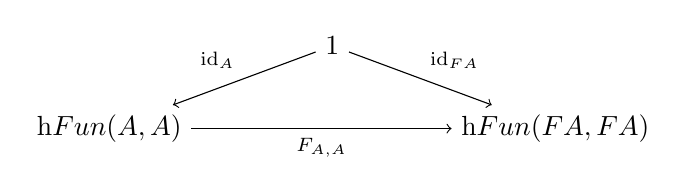
\begin{tikzpicture}[x=1.3em,y=1.3em]
  \node (1u) at (0,2.3) {$\mathbb{1}$};
  \node (l) at (-6.2,0) {$\mathrm{h}\Fun(A,A)$};
  \node (r) at (6.2,0) {$\mathrm{h}\Fun(FA,FA)$};
  \draw[->] (1u) -- node[above left]{$\scriptstyle\mathrm{id}_{A}$} (l);
  \draw[->] (1u) -- node[above right]{$\scriptstyle\mathrm{id}_{FA}$} (r);
  \draw[->] (l) -- node[below]{$\scriptstyle F_{A,A}$} (r);
\end{tikzpicture}
\par\vspace{0.8em}
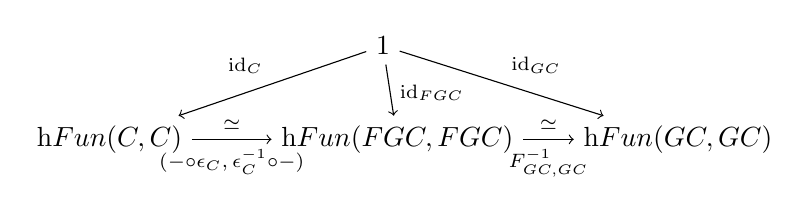
\begin{tikzpicture}[x=1.3em,y=1.3em]
  \node (1u) at (0,2.6) {$\mathbb{1}$};
  \node (l) at (-7.6,0) {$\mathrm{h}\Fun(C,C)$};
  \node (m) at (0.4,0) {$\mathrm{h}\Fun(FGC,FGC)$};
  \node (r) at (8.2,0) {$\mathrm{h}\Fun(GC,GC)$};
  \draw[->] (1u) -- node[above left]{$\scriptstyle\mathrm{id}_{C}$} (l);
  \draw[->] (1u) -- node[above right]{$\scriptstyle\mathrm{id}_{GC}$} (r);
  \draw[->] (1u) -- node[right,pos=0.55]{$\scriptstyle\mathrm{id}_{FGC}$} (m);
  \draw[->] (l) -- node[above]{$\scriptstyle\simeq$}
    node[below]{$\scriptstyle(-\circ\epsilon_{C},\,\epsilon_{C}^{-1}\circ-)$} (m);
  \draw[->] (m) -- node[above]{$\scriptstyle\simeq$}
    node[below]{$\scriptstyle F_{GC,GC}^{-1}$} (r);
\end{tikzpicture}
\end{center}

取而代之，映射 $G\colon\mathfrak{h}\mathcal{L}\rightsquigarrow\mathfrak{h}\mathcal{K}$
在诸\trHomotopyTwoCategory{}之间定义一个伪函子，这一概念我们现在予以回顾。

\begin{definition}\label{def:pseudofunctor}
介于 2-\trCategory{} $\mathcal{C}$ 与 $\mathcal{D}$ 之间的一个\textbf{伪函子}
$G\colon\mathcal{C}\rightsquigarrow\mathcal{D}$ 由如下数据给出：
\begin{itemize}
\item 对象上的一个映射 $\mathcal{C}\ni x\mapsto Gx\in\mathcal{D}$；
\item 对每一对 $x$、$y\in\mathcal{C}$，hom-\trCategory{}上的一个映射
$G_{x,y}\colon\mathcal{C}(x,y)\to\mathcal{D}(Gx,Gy)$；

\item 对每个 $x\in\mathcal{C}$，一个可逆 2-\trCell
\begin{center}
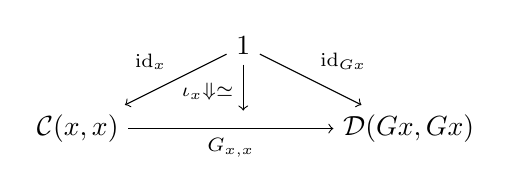
\begin{tikzpicture}[x=1.3em,y=1.3em]
  \node (1u) at (0,2.3) {$\mathbb{1}$};
  \node (l) at (-4.6,0) {$\mathcal{C}(x,x)$};
  \node (r) at (4.6,0) {$\mathcal{D}(Gx,Gx)$};
  \draw[->] (1u) -- node[above left]{$\scriptstyle\mathrm{id}_{x}$} (l);
  \draw[->] (1u) -- node[above right]{$\scriptstyle\mathrm{id}_{Gx}$} (r);
  \draw[->] (l) -- node[below]{$\scriptstyle G_{x,x}$} (r);
  \draw[->] (1u) -- node[left,pos=0.6]{$\scriptstyle\iota_{x}\Downarrow\simeq$} (0,0.5);
\end{tikzpicture}
\end{center}
它定义 $\mathcal{D}(Gx,Gx)$ 中的一个\trIsomorphism{}
$\iota_{x}\colon\mathrm{id}_{Gx}\cong G\,\mathrm{id}_{x}$\footnote{原书印作
「$G\,\mathrm{id}_{X}$」，末位系大写斜体 $X$；本条全句量词仅约束小写 $x$，且
其余诸处均作小写，应为排版笔误，此处径改。——译者注}；以及
\item 对每一三元组对象 $x$、$y$、$z\in\mathcal{C}$，一个自然同构
\begin{center}
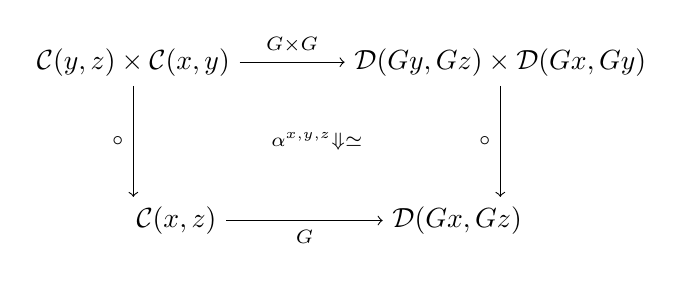
\begin{tikzpicture}[x=1.3em,y=1.3em]
  \node (tl) at (-4.8,2.2) {$\mathcal{C}(y,z)\times\mathcal{C}(x,y)$};
  \node (tr) at (5.4,2.2) {$\mathcal{D}(Gy,Gz)\times\mathcal{D}(Gx,Gy)$};
  \node (bl) at (-3.6,-2.2) {$\mathcal{C}(x,z)$};
  \node (br) at (4.2,-2.2) {$\mathcal{D}(Gx,Gz)$};
  \draw[->] (tl) -- node[above]{$\scriptstyle G{\times}G$} (tr);
  \draw[->] (bl) -- node[below]{$\scriptstyle G$} (br);
  \draw[->] (tl.south) -- node[left]{$\scriptstyle\circ$} (tl.south |- bl.north);
  \draw[->] (tr.south) -- node[left]{$\scriptstyle\circ$} (tr.south |- br.north);
  \node at (0.3,0) {$\scriptstyle\alpha^{x,y,z}\Downarrow\simeq$};
\end{tikzpicture}
\end{center}
满足由诸粘贴等式所编码的三条相干条件：
\begin{center}
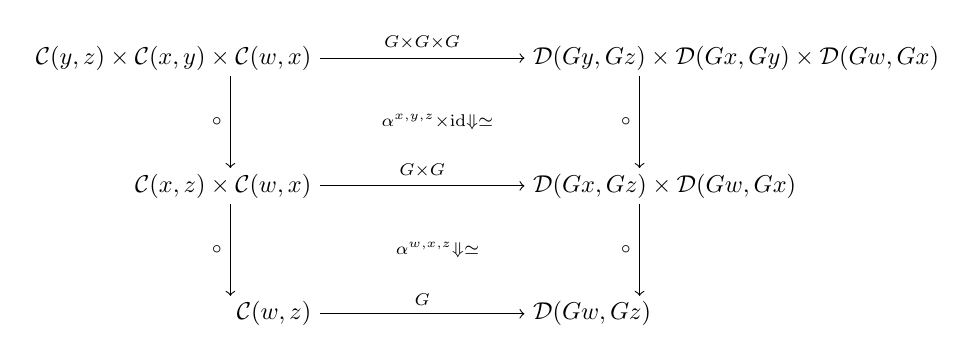
\begin{tikzpicture}[x=1.05em,y=1.05em,scale=0.88,transform shape]
  \node[anchor=east] (r1l) at (0,5) {$\mathcal{C}(y,z)\times\mathcal{C}(x,y)\times\mathcal{C}(w,x)$};
  \node[anchor=west] (r1r) at (8,5) {$\mathcal{D}(Gy,Gz)\times\mathcal{D}(Gx,Gy)\times\mathcal{D}(Gw,Gx)$};
  \node[anchor=east] (r2l) at (0,0) {$\mathcal{C}(x,z)\times\mathcal{C}(w,x)$};
  \node[anchor=west] (r2r) at (8,0) {$\mathcal{D}(Gx,Gz)\times\mathcal{D}(Gw,Gx)$};
  \node[anchor=east] (r3l) at (0,-5) {$\mathcal{C}(w,z)$};
  \node[anchor=west] (r3r) at (8,-5) {$\mathcal{D}(Gw,Gz)$};
  \draw[->] (r1l.east) -- node[above]{$\scriptstyle G{\times}G{\times}G$} (r1r.west);
  \draw[->] (r2l.east) -- node[above]{$\scriptstyle G{\times}G$} (r2r.west);
  \draw[->] (r3l.east) -- node[above]{$\scriptstyle G$} (r3r.west);
  \draw[->] (-3.5,4.3) -- node[left]{$\scriptstyle\circ$} (-3.5,0.7);
  \draw[->] (12.5,4.3) -- node[left]{$\scriptstyle\circ$} (12.5,0.7);
  \draw[->] (-3.5,-0.7) -- node[left]{$\scriptstyle\circ$} (-3.5,-4.3);
  \draw[->] (12.5,-0.7) -- node[left]{$\scriptstyle\circ$} (12.5,-4.3);
  \node at (4.6,2.5) {$\scriptstyle\alpha^{x,y,z}\times\mathrm{id}\Downarrow\simeq$};
  \node at (4.6,-2.5) {$\scriptstyle\alpha^{w,x,z}\Downarrow\simeq$};
\end{tikzpicture}
\par\vspace{0.5em}
\begin{tikzpicture}
  \draw[double,double distance=1.2pt] (0,0)--(0,0.75);
\end{tikzpicture}
\par\vspace{0.5em}
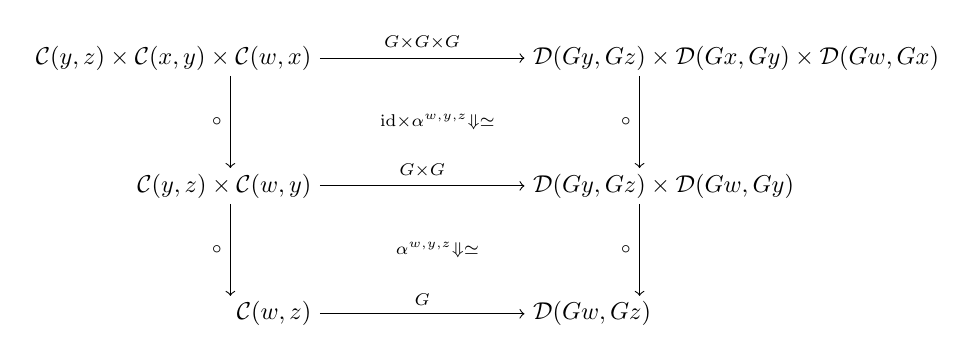
\begin{tikzpicture}[x=1.05em,y=1.05em,scale=0.88,transform shape]
  \node[anchor=east] (r1l) at (0,5) {$\mathcal{C}(y,z)\times\mathcal{C}(x,y)\times\mathcal{C}(w,x)$};
  \node[anchor=west] (r1r) at (8,5) {$\mathcal{D}(Gy,Gz)\times\mathcal{D}(Gx,Gy)\times\mathcal{D}(Gw,Gx)$};
  \node[anchor=east] (r2l) at (0,0) {$\mathcal{C}(y,z)\times\mathcal{C}(w,y)$};
  \node[anchor=west] (r2r) at (8,0) {$\mathcal{D}(Gy,Gz)\times\mathcal{D}(Gw,Gy)$};
  \node[anchor=east] (r3l) at (0,-5) {$\mathcal{C}(w,z)$};
  \node[anchor=west] (r3r) at (8,-5) {$\mathcal{D}(Gw,Gz)$};
  \draw[->] (r1l.east) -- node[above]{$\scriptstyle G{\times}G{\times}G$} (r1r.west);
  \draw[->] (r2l.east) -- node[above]{$\scriptstyle G{\times}G$} (r2r.west);
  \draw[->] (r3l.east) -- node[above]{$\scriptstyle G$} (r3r.west);
  \draw[->] (-3.5,4.3) -- node[left]{$\scriptstyle\circ$} (-3.5,0.7);
  \draw[->] (12.5,4.3) -- node[left]{$\scriptstyle\circ$} (12.5,0.7);
  \draw[->] (-3.5,-0.7) -- node[left]{$\scriptstyle\circ$} (-3.5,-4.3);
  \draw[->] (12.5,-0.7) -- node[left]{$\scriptstyle\circ$} (12.5,-4.3);
  \node at (4.6,2.5) {$\scriptstyle\mathrm{id}\times\alpha^{w,y,z}\Downarrow\simeq$};
  \node at (4.6,-2.5) {$\scriptstyle\alpha^{w,y,z}\Downarrow\simeq$};
\end{tikzpicture}
\end{center}
\begin{center}
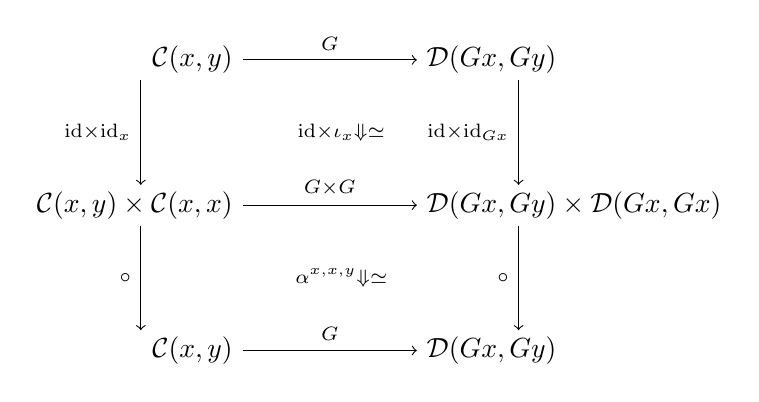
\begin{tikzpicture}[x=1.05em,y=1.05em]
  \node[anchor=east] (r1l) at (0,5) {$\mathcal{C}(x,y)$};
  \node[anchor=west] (r1r) at (6,5) {$\mathcal{D}(Gx,Gy)$};
  \node[anchor=east] (r2l) at (0,0) {$\mathcal{C}(x,y)\times\mathcal{C}(x,x)$};
  \node[anchor=west] (r2r) at (6,0) {$\mathcal{D}(Gx,Gy)\times\mathcal{D}(Gx,Gx)$};
  \node[anchor=east] (r3l) at (0,-5) {$\mathcal{C}(x,y)$};
  \node[anchor=west] (r3r) at (6,-5) {$\mathcal{D}(Gx,Gy)$};
  \draw[->] (r1l.east) -- node[above]{$\scriptstyle G$} (r1r.west);
  \draw[->] (r2l.east) -- node[above]{$\scriptstyle G{\times}G$} (r2r.west);
  \draw[->] (r3l.east) -- node[above]{$\scriptstyle G$} (r3r.west);
  \draw[->] (-3.5,4.3) -- node[left]{$\scriptstyle\mathrm{id}{\times}\mathrm{id}_{x}$} (-3.5,0.7);
  \draw[->] (9.5,4.3) -- node[left]{$\scriptstyle\mathrm{id}{\times}\mathrm{id}_{Gx}$} (9.5,0.7);
  \draw[->] (-3.5,-0.7) -- node[left]{$\scriptstyle\circ$} (-3.5,-4.3);
  \draw[->] (9.5,-0.7) -- node[left]{$\scriptstyle\circ$} (9.5,-4.3);
  \node at (3.4,2.5) {$\scriptstyle\mathrm{id}{\times}\iota_{x}\Downarrow\simeq$};
  \node at (3.4,-2.5) {$\scriptstyle\alpha^{x,x,y}\Downarrow\simeq$};
\end{tikzpicture}
\par\vspace{0.5em}
\begin{tikzpicture}
  \draw[double,double distance=1.2pt] (0,0)--(0,0.75);
\end{tikzpicture}
\par\vspace{0.5em}
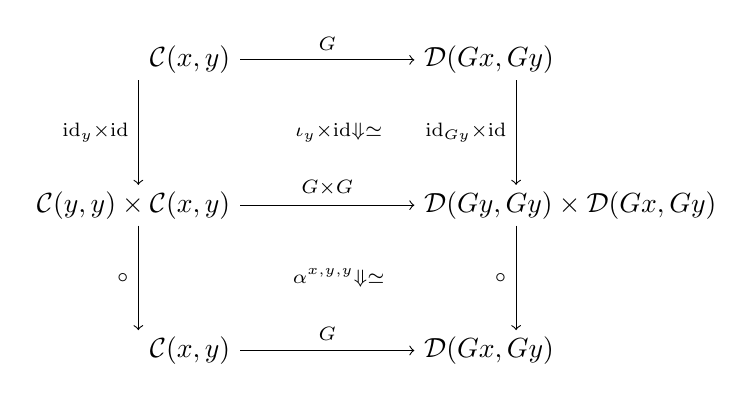
\begin{tikzpicture}[x=1.05em,y=1.05em]
  \node[anchor=east] (r1l) at (0,5) {$\mathcal{C}(x,y)$};
  \node[anchor=west] (r1r) at (6,5) {$\mathcal{D}(Gx,Gy)$};
  \node[anchor=east] (r2l) at (0,0) {$\mathcal{C}(y,y)\times\mathcal{C}(x,y)$};
  \node[anchor=west] (r2r) at (6,0) {$\mathcal{D}(Gy,Gy)\times\mathcal{D}(Gx,Gy)$};
  \node[anchor=east] (r3l) at (0,-5) {$\mathcal{C}(x,y)$};
  \node[anchor=west] (r3r) at (6,-5) {$\mathcal{D}(Gx,Gy)$};
  \draw[->] (r1l.east) -- node[above]{$\scriptstyle G$} (r1r.west);
  \draw[->] (r2l.east) -- node[above]{$\scriptstyle G{\times}G$} (r2r.west);
  \draw[->] (r3l.east) -- node[above]{$\scriptstyle G$} (r3r.west);
  \draw[->] (-3.5,4.3) -- node[left]{$\scriptstyle\mathrm{id}_{y}{\times}\mathrm{id}$} (-3.5,0.7);
  \draw[->] (9.5,4.3) -- node[left]{$\scriptstyle\mathrm{id}_{Gy}{\times}\mathrm{id}$} (9.5,0.7);
  \draw[->] (-3.5,-0.7) -- node[left]{$\scriptstyle\circ$} (-3.5,-4.3);
  \draw[->] (9.5,-0.7) -- node[left]{$\scriptstyle\circ$} (9.5,-4.3);
  \node at (3.4,2.5) {$\scriptstyle\iota_{y}{\times}\mathrm{id}\Downarrow\simeq$};
  \node at (3.4,-2.5) {$\scriptstyle\alpha^{x,y,y}\Downarrow\simeq$};
\end{tikzpicture}
\end{center}
其中这两个后者的复合均等于单位 2-\trCell{}
$\mathrm{id}_{G_{x,y}}$。
\end{itemize}
\end{definition}

一个\textbf{2-\trFunctor}是这样的伪函子：其中单位胞腔与复合胞腔 $\iota$ 与
$\alpha$ 均为恒同。2-\trFunctor{}之间的 2-自然变换（见附录 B 中的%
\cref{def:two-natural-transformation}）这一概念，
同样地推广为伪函子之间的伪自然变换。

\begin{definition}\label{def:pseudonatural-transformation}
对任意一对 2-\trCategory{} $\mathcal{C}$ 与 $\mathcal{D}$ 以及平行的伪函子
$F$、$G\colon\mathcal{C}\rightsquigarrow\mathcal{D}$，一个\textbf{伪自然变换}
$\phi\colon F\Rrightarrow G$ 由如下数据给出：
\begin{itemize}
\item 对每个对象 $x\in\mathcal{C}$，一个 1-\trCell{}
$\phi_{x}\colon Fx\to Gx\in\mathcal{D}$；并且
\item 对每个 1-\trCell{} $f\colon x\to y\in\mathcal{C}$，$\mathcal{D}$ 中的一个
可逆 2-\trCell
\begin{center}
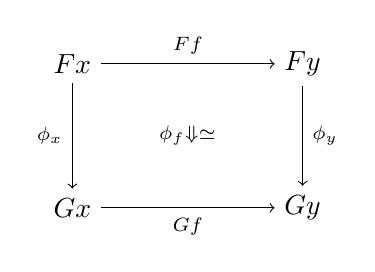
\begin{tikzpicture}[x=1.3em,y=1.3em]
  \node (tl) at (-3.2,2) {$Fx$};
  \node (tr) at (3.2,2) {$Fy$};
  \node (bl) at (-3.2,-2) {$Gx$};
  \node (br) at (3.2,-2) {$Gy$};
  \draw[->] (tl) -- node[above]{$\scriptstyle Ff$} (tr);
  \draw[->] (bl) -- node[below]{$\scriptstyle Gf$} (br);
  \draw[->] (tl) -- node[left]{$\scriptstyle\phi_{x}$} (bl);
  \draw[->] (tr) -- node[right]{$\scriptstyle\phi_{y}$} (br);
  \node at (0,0) {$\scriptstyle\phi_{f}\Downarrow\simeq$};
\end{tikzpicture}
\end{center}
使得这批数据
\item 是自然的，其意义为：对 $\mathcal{C}$ 中的每个 2-\trCell{}
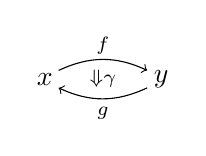
\begin{tikzpicture}[x=1em,y=0.9em,baseline=-0.5em]
  \node (x) at (0,0) {$x$};
  \node (y) at (4.2,0) {$y$};
  \draw[->] (0.5,0.35) to[bend left=25] (3.7,0.35);
  \node at (2.1,1.35) {$\scriptstyle f$};
  \draw[->] (3.7,-0.35) to[bend left=25] (0.5,-0.35);
  \node at (2.1,-1.35) {$\scriptstyle g$};
  \node at (2.1,0) {$\scriptstyle\Downarrow\gamma$};
\end{tikzpicture}
（$\mathcal{C}$ 中），粘贴复合相等
\begin{center}
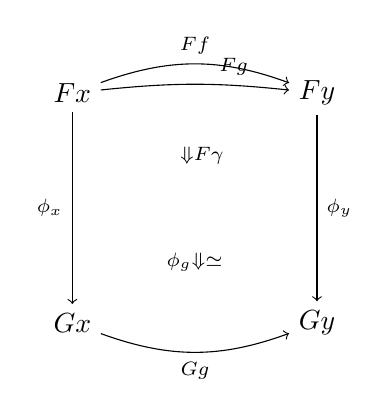
\begin{tikzpicture}[x=1.3em,y=1.3em]
  \node (tl) at (-3.4,3.2) {$Fx$};
  \node (tr) at (3.4,3.2) {$Fy$};
  \node (bl) at (-3.4,-3.2) {$Gx$};
  \node (br) at (3.4,-3.2) {$Gy$};
  \draw[->] (tl) to[bend left=20] node[above]{$\scriptstyle Ff$} (tr);
  \draw[->] (tl) to[bend left=6] node[above,pos=0.72]{$\scriptstyle Fg$} (tr);
  \node at (0.2,1.45) {$\scriptstyle\Downarrow F\gamma$};
  \draw[->] (tl) -- node[left]{$\scriptstyle\phi_{x}$} (bl);
  \draw[->] (tr) -- node[right]{$\scriptstyle\phi_{y}$} (br);
  \node at (0,-1.5) {$\scriptstyle\phi_{g}\Downarrow\simeq$};
  \draw[->] (bl) to[bend right=20] node[below]{$\scriptstyle Gg$} (br);
\end{tikzpicture}
\quad$=$\quad
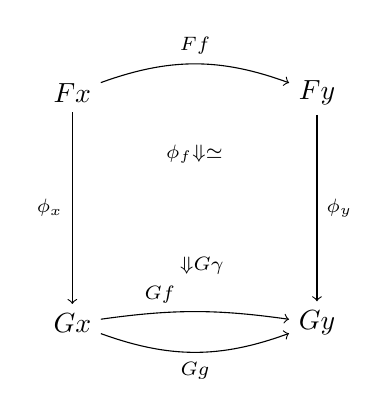
\begin{tikzpicture}[x=1.3em,y=1.3em]
  \node (tl) at (-3.4,3.2) {$Fx$};
  \node (tr) at (3.4,3.2) {$Fy$};
  \node (bl) at (-3.4,-3.2) {$Gx$};
  \node (br) at (3.4,-3.2) {$Gy$};
  \draw[->] (tl) to[bend left=20] node[above]{$\scriptstyle Ff$} (tr);
  \node at (0,1.5) {$\scriptstyle\phi_{f}\Downarrow\simeq$};
  \draw[->] (tl) -- node[left]{$\scriptstyle\phi_{x}$} (bl);
  \draw[->] (tr) -- node[right]{$\scriptstyle\phi_{y}$} (br);
  \draw[->] (bl) to[bend left=8] node[above,pos=0.3]{$\scriptstyle Gf$} (br);
  \node at (0.2,-1.6) {$\scriptstyle\Downarrow G\gamma$};
  \draw[->] (bl) to[bend right=20] node[below]{$\scriptstyle Gg$} (br);
\end{tikzpicture}
\end{center}
；以及
\item 尊重由诸伪函子指定的复合约束与单位约束：
\begin{center}
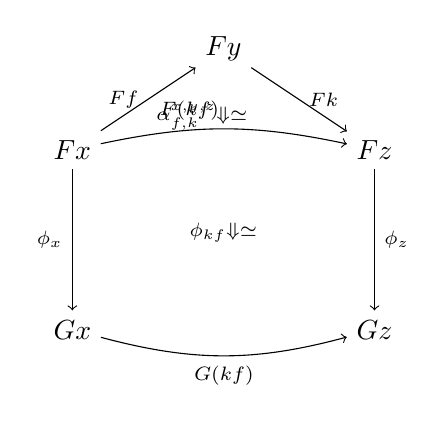
\begin{tikzpicture}[x=1.3em,y=1.3em]
  \node (fx) at (-4.2,0.6) {$Fx$};
  \node (fy) at (0,3.4) {$Fy$};
  \node (fz) at (4.2,0.6) {$Fz$};
  \node (gx) at (-4.2,-4.4) {$Gx$};
  \node (gz) at (4.2,-4.4) {$Gz$};
  \draw[->] (fx) -- node[above,left]{$\scriptstyle Ff$} (fy);
  \draw[->] (fy) -- node[above,right]{$\scriptstyle Fk$} (fz);
  \node at (-0.6,1.5) {$\scriptstyle\alpha^{x,y,z}_{f,k}\Downarrow\simeq$};
  \draw[->] (fx) to[bend left=12] node[above,pos=0.35]{$\scriptstyle F(kf)$} (fz);
  \node at (0,-1.7) {$\scriptstyle\phi_{kf}\Downarrow\simeq$};
  \draw[->] (fx) -- node[left]{$\scriptstyle\phi_{x}$} (gx);
  \draw[->] (fz) -- node[right]{$\scriptstyle\phi_{z}$} (gz);
  \draw[->] (gx) to[bend right=15] node[below]{$\scriptstyle G(kf)$} (gz);
\end{tikzpicture}
\quad$=$\quad
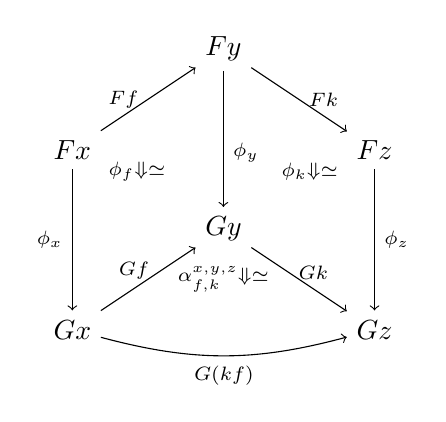
\begin{tikzpicture}[x=1.3em,y=1.3em]
  \node (fx) at (-4.2,0.6) {$Fx$};
  \node (fy) at (0,3.4) {$Fy$};
  \node (fz) at (4.2,0.6) {$Fz$};
  \node (gx) at (-4.2,-4.4) {$Gx$};
  \node (gy) at (0,-1.6) {$Gy$};
  \node (gz) at (4.2,-4.4) {$Gz$};
  \draw[->] (fx) -- node[above,left]{$\scriptstyle Ff$} (fy);
  \draw[->] (fy) -- node[above,right]{$\scriptstyle Fk$} (fz);
  \draw[->] (fx) -- node[left]{$\scriptstyle\phi_{x}$} (gx);
  \draw[->] (fy) -- node[right,pos=0.6]{$\scriptstyle\phi_{y}$} (gy);
  \draw[->] (fz) -- node[right]{$\scriptstyle\phi_{z}$} (gz);
  \node at (-2.4,0) {$\scriptstyle\phi_{f}\Downarrow\simeq$};
  \node at (2.4,0) {$\scriptstyle\phi_{k}\Downarrow\simeq$};
  \draw[->] (gx) -- node[above,pos=0.35]{$\scriptstyle Gf$} (gy);
  \draw[->] (gy) -- node[above,pos=0.65]{$\scriptstyle Gk$} (gz);
  \node at (0,-3.0) {$\scriptstyle\alpha^{x,y,z}_{f,k}\Downarrow\simeq$};
  \draw[->] (gx) to[bend right=15] node[below]{$\scriptstyle G(kf)$} (gz);
\end{tikzpicture}
\end{center}
\par 以及
\begin{center}
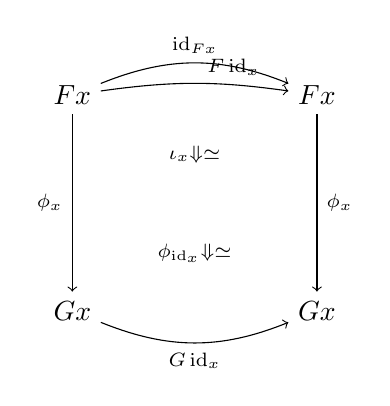
\begin{tikzpicture}[x=1.3em,y=1.3em]
  \node (tl) at (-3.4,3.0) {$Fx$};
  \node (tr) at (3.4,3.0) {$Fx$};
  \node (bl) at (-3.4,-3.0) {$Gx$};
  \node (br) at (3.4,-3.0) {$Gx$};
  \draw[->] (tl) to[bend left=22] node[above]{$\scriptstyle\mathrm{id}_{Fx}$} (tr);
  \draw[->] (tl) to[bend left=8] node[above,pos=0.72]{$\scriptstyle F\,\mathrm{id}_{x}$} (tr);
  \node at (0,1.35) {$\scriptstyle\iota_{x}\Downarrow\simeq$};
  \draw[->] (tl) -- node[left]{$\scriptstyle\phi_{x}$} (bl);
  \draw[->] (tr) -- node[right]{$\scriptstyle\phi_{x}$} (br);
  \node at (0,-1.4) {$\scriptstyle\phi_{\mathrm{id}_{x}}\Downarrow\simeq$};
  \draw[->] (bl) to[bend right=22] node[below]{$\scriptstyle G\,\mathrm{id}_{x}$} (br);
\end{tikzpicture}
\quad$=$\quad
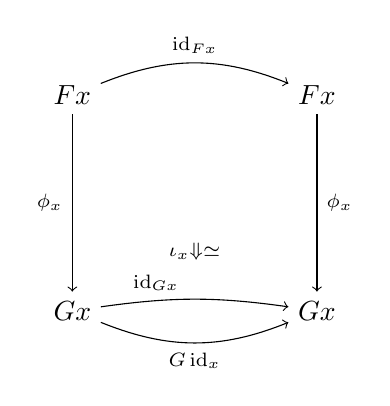
\begin{tikzpicture}[x=1.3em,y=1.3em]
  \node (tl) at (-3.4,3.0) {$Fx$};
  \node (tr) at (3.4,3.0) {$Fx$};
  \node (bl) at (-3.4,-3.0) {$Gx$};
  \node (br) at (3.4,-3.0) {$Gx$};
  \draw[->] (tl) to[bend left=22] node[above]{$\scriptstyle\mathrm{id}_{Fx}$} (tr);
  \draw[->] (tl) -- node[left]{$\scriptstyle\phi_{x}$} (bl);
  \draw[->] (tr) -- node[right]{$\scriptstyle\phi_{x}$} (br);
  \draw[->] (bl) to[bend left=8] node[above,pos=0.28]{$\scriptstyle\mathrm{id}_{Gx}$} (br);
  \node at (0,-1.35) {$\scriptstyle\iota_{x}\Downarrow\simeq$};
  \draw[->] (bl) to[bend right=22] node[below]{$\scriptstyle G\,\mathrm{id}_{x}$} (br);
\end{tikzpicture}
\footnote{原书此图之中部 2-胞腔印作「$\iota_{y}\Downarrow\simeq$」，然图中诸对象
皆为 $x$，按单位胞腔语义系 $G$ 在 $x$ 处之单位 2-胞腔 $\iota_{x}$，此处径改。——译者注}
\end{center}
\end{itemize}
\end{definition}

伪函子浮现的一个语境，是作为定义\trBiequivalence{}的 2-\trFunctor{}之逆。
以此方式浮现的伪函子本身是\textbf{双等价的}：依等价意义于对象上为满，并且在
hom-\trCategory{}上定义\trLocalEquivalence。这些\trFunctor{}是逆，其意义为：
在各复合与诸恒同之间存在\textbf{伪自然等价}——即逐分量地成为\trEquivalence{}的
伪自然变换（另一刻画见\cref{ex:pseudonatural-equivalence-characterization}）。
总体而言，这批数据定义了 2-\trCategory{}%
在适合于\trBicategory{}理论之意义上的一个\trEquivalence：

\begin{proposition}\label{prop:pseudoinverse-2-functor}
若 $F\colon\mathcal{C}\to\mathcal{D}$ 是 2-\trCategory{} $\mathcal{C}$ 与
$\mathcal{D}$ 之间的一个 2-\trFunctor{}兼\trBiequivalence，则存在一个伪函子
$G\colon\mathcal{D}\rightsquigarrow\mathcal{C}$，它也是\trBiequivalence，并且在
下述意义下是 $F$ 的一个\emph{伪逆}（pseudoinverse）：存在伪自然等价
$\mathrm{id}_{\mathcal{C}}\Rrightarrow GF$ 与
$FG\Rrightarrow\mathrm{id}_{\mathcal{D}}$。
\end{proposition}

\begin{proof}
\cref{ex:derive-prop-1043}。
\end{proof}

命题 10.4.3 描述了\trBicategory{}理论中的一个经典结果，Johnson 与 Yau 称之为%
「\trBicategory{} Whitehead 定理」[59, 7.4.1]，所以我们心安理得地把它的证明留给练习（亦见%
\cref{prop:quasi-pseudoinverse}）。

请回忆定义 1.2.1：一个\trInfinityCosmos{}除其他外，是一个在诸\trQuasiCategory{}之%
\trCartesianClosed\trCategory{}中富集的\trCategory；而一支\trCosmologicalFunctor{}除其他外，
是诸拟范畴富集\trCategory{}之间的一个富集\trFunctor{}（见 A.2 节）。
为定义一个拟范畴富集伪函子，我们需要把由\trQuasiCategory{}与\trFunctor{}构成的
1-\trCategory{}扩张为一座 2-\trCategory，从而可以利用它的 2-\trCell{}来编码单位
相干与复合相干。幸运的是，我们手头正有这样一座 2-\trCategory：\trQuasiCategory{}的%
\trHomotopyTwoCategory{} $\mathfrak{h}\QCat$。由命题 1.4.5，这座由拟范畴、其间的%
\trFunctor{}以及其间的\trNaturalTransformation{}构成的 2-\trCategory{}是%
\trCartesianClosed{}，于是我们在这些 2-\trCell{}上拥有良态的\trCartesianProduct{}与
转置运算。

$\mathfrak{h}\QCat$ 这座 2-\trCategory{}中的额外维数，使我们能够如下定义拟范畴
富集伪函子：

\begin{definition}\label{def:quasi-pseudofunctor}
对诸拟范畴富集\trCategory{} $\mathcal{K}$ 与 $\mathcal{L}$，一个\textbf{拟范畴
富集伪函子} $G\colon\mathcal{K}\rightsquigarrow\mathcal{L}$——简称\textbf{拟伪函子}
——由如下数据给出：
\begin{itemize}
\item 对象上的一个映射 $\mathcal{K}\ni x\mapsto Gx\in\mathcal{L}$；
\item 对每一对 $x$、$y\in\mathcal{K}$，hom-\trQuasiCategory{}之间的一个\trFunctor{}
$G_{x,y}\colon\mathcal{K}(x,y)\to\mathcal{L}(Gx,Gy)$；
\item 对每个 $x\in\mathcal{K}$，在诸\trQuasiCategory{}的\trHomotopyTwoCategory{}中的一个
可逆 2-\trCell
\begin{center}
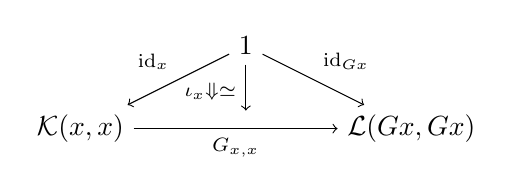
\begin{tikzpicture}[x=1.3em,y=1.3em]
  \node (1u) at (0,2.3) {$\mathbb{1}$};
  \node (l) at (-4.6,0) {$\mathcal{K}(x,x)$};
  \node (r) at (4.6,0) {$\mathcal{L}(Gx,Gx)$};
  \draw[->] (1u) -- node[above left]{$\scriptstyle\mathrm{id}_{x}$} (l);
  \draw[->] (1u) -- node[above right]{$\scriptstyle\mathrm{id}_{Gx}$} (r);
  \draw[->] (l) -- node[below]{$\scriptstyle G_{x,x}$} (r);
  \draw[->] (1u) -- node[left,pos=0.6]{$\scriptstyle\iota_{x}\Downarrow\simeq$} (0,0.5);
\end{tikzpicture}
\end{center}
\item 对每一三元组对象 $x$、$y$、$z\in\mathcal{K}$，在诸拟范畴的%
\trHomotopyTwoCategory{}中的一个可逆 2-\trCell
\begin{center}
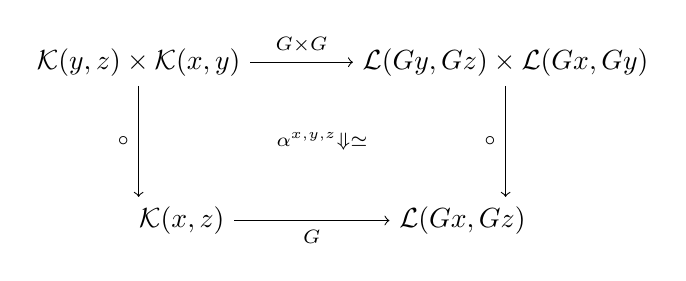
\begin{tikzpicture}[x=1.3em,y=1.3em]
  \node (tl) at (-4.8,2.2) {$\mathcal{K}(y,z)\times\mathcal{K}(x,y)$};
  \node (tr) at (5.4,2.2) {$\mathcal{L}(Gy,Gz)\times\mathcal{L}(Gx,Gy)$};
  \node (bl) at (-3.6,-2.2) {$\mathcal{K}(x,z)$};
  \node (br) at (4.2,-2.2) {$\mathcal{L}(Gx,Gz)$};
  \draw[->] (tl) -- node[above]{$\scriptstyle G{\times}G$} (tr);
  \draw[->] (bl) -- node[below]{$\scriptstyle G$} (br);
  \draw[->] (tl.south) -- node[left]{$\scriptstyle\circ$} (tl.south |- bl.north);
  \draw[->] (tr.south) -- node[left]{$\scriptstyle\circ$} (tr.south |- br.north);
  \node at (0.3,0) {$\scriptstyle\alpha^{x,y,z}\Downarrow\simeq$};
\end{tikzpicture}
\end{center}

满足由诸粘贴等式所编码的三条相干条件：
\begin{rveq}\label{eq:quasi-pseudofunctor-pasting}
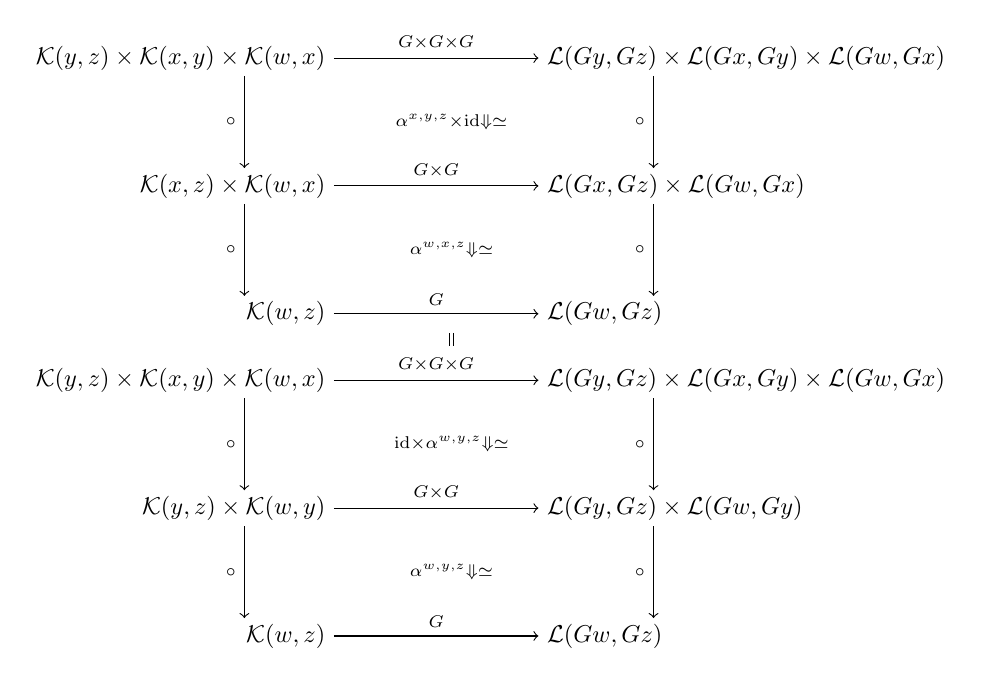
\begin{tikzpicture}[x=1.05em,y=1.05em,scale=0.88,transform shape]
  \node[anchor=east] (r1l) at (0,5) {$\mathcal{K}(y,z)\times\mathcal{K}(x,y)\times\mathcal{K}(w,x)$};
  \node[anchor=west] (r1r) at (8,5) {$\mathcal{L}(Gy,Gz)\times\mathcal{L}(Gx,Gy)\times\mathcal{L}(Gw,Gx)$};
  \node[anchor=east] (r2l) at (0,0) {$\mathcal{K}(x,z)\times\mathcal{K}(w,x)$};
  \node[anchor=west] (r2r) at (8,0) {$\mathcal{L}(Gx,Gz)\times\mathcal{L}(Gw,Gx)$};
  \node[anchor=east] (r3l) at (0,-5) {$\mathcal{K}(w,z)$};
  \node[anchor=west] (r3r) at (8,-5) {$\mathcal{L}(Gw,Gz)$};
  \draw[->] (r1l.east) -- node[above]{$\scriptstyle G{\times}G{\times}G$} (r1r.west);
  \draw[->] (r2l.east) -- node[above]{$\scriptstyle G{\times}G$} (r2r.west);
  \draw[->] (r3l.east) -- node[above]{$\scriptstyle G$} (r3r.west);
  \draw[->] (-3.5,4.3) -- node[left]{$\scriptstyle\circ$} (-3.5,0.7);
  \draw[->] (12.5,4.3) -- node[left]{$\scriptstyle\circ$} (12.5,0.7);
  \draw[->] (-3.5,-0.7) -- node[left]{$\scriptstyle\circ$} (-3.5,-4.3);
  \draw[->] (12.5,-0.7) -- node[left]{$\scriptstyle\circ$} (12.5,-4.3);
  \node at (4.6,2.5) {$\scriptstyle\alpha^{x,y,z}\times\mathrm{id}\Downarrow\simeq$};
  \node at (4.6,-2.5) {$\scriptstyle\alpha^{w,x,z}\Downarrow\simeq$};
  \draw[double,double distance=1.2pt] (4.6,-5.75) -- (4.6,-6.25);
  \node[anchor=east] (r1l) at (0,-7.6) {$\mathcal{K}(y,z)\times\mathcal{K}(x,y)\times\mathcal{K}(w,x)$};
  \node[anchor=west] (r1r) at (8,-7.6) {$\mathcal{L}(Gy,Gz)\times\mathcal{L}(Gx,Gy)\times\mathcal{L}(Gw,Gx)$};
  \node[anchor=east] (r2l) at (0,-12.6) {$\mathcal{K}(y,z)\times\mathcal{K}(w,y)$};
  \node[anchor=west] (r2r) at (8,-12.6) {$\mathcal{L}(Gy,Gz)\times\mathcal{L}(Gw,Gy)$};
  \node[anchor=east] (r3l) at (0,-17.6) {$\mathcal{K}(w,z)$};
  \node[anchor=west] (r3r) at (8,-17.6) {$\mathcal{L}(Gw,Gz)$};
  \draw[->] (r1l.east) -- node[above]{$\scriptstyle G{\times}G{\times}G$} (r1r.west);
  \draw[->] (r2l.east) -- node[above]{$\scriptstyle G{\times}G$} (r2r.west);
  \draw[->] (r3l.east) -- node[above]{$\scriptstyle G$} (r3r.west);
  \draw[->] (-3.5,-8.3) -- node[left]{$\scriptstyle\circ$} (-3.5,-11.9);
  \draw[->] (12.5,-8.3) -- node[left]{$\scriptstyle\circ$} (12.5,-11.9);
  \draw[->] (-3.5,-13.3) -- node[left]{$\scriptstyle\circ$} (-3.5,-16.9);
  \draw[->] (12.5,-13.3) -- node[left]{$\scriptstyle\circ$} (12.5,-16.9);
  \node at (4.6,-10.1) {$\scriptstyle\mathrm{id}{\times}\alpha^{w,y,z}\Downarrow\simeq$};
  \node at (4.6,-15.1) {$\scriptstyle\alpha^{w,y,z}\Downarrow\simeq$};
\end{tikzpicture}
\end{rveq}
\begin{center}
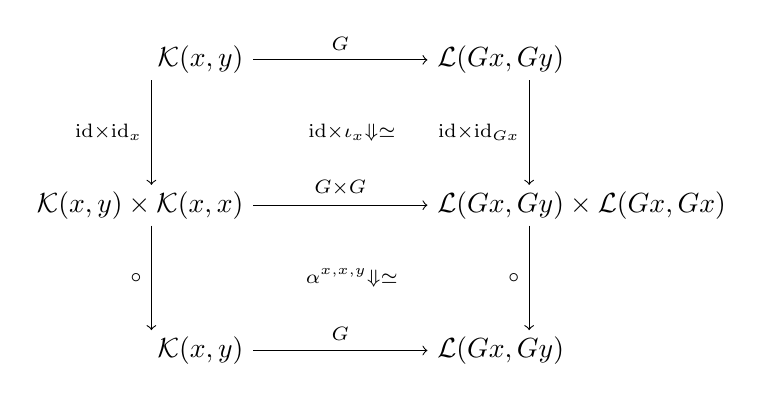
\begin{tikzpicture}[x=1.05em,y=1.05em]
  \node[anchor=east] (r1l) at (0,5) {$\mathcal{K}(x,y)$};
  \node[anchor=west] (r1r) at (6,5) {$\mathcal{L}(Gx,Gy)$};
  \node[anchor=east] (r2l) at (0,0) {$\mathcal{K}(x,y)\times\mathcal{K}(x,x)$};
  \node[anchor=west] (r2r) at (6,0) {$\mathcal{L}(Gx,Gy)\times\mathcal{L}(Gx,Gx)$};
  \node[anchor=east] (r3l) at (0,-5) {$\mathcal{K}(x,y)$};
  \node[anchor=west] (r3r) at (6,-5) {$\mathcal{L}(Gx,Gy)$};
  \draw[->] (r1l.east) -- node[above]{$\scriptstyle G$} (r1r.west);
  \draw[->] (r2l.east) -- node[above]{$\scriptstyle G{\times}G$} (r2r.west);
  \draw[->] (r3l.east) -- node[above]{$\scriptstyle G$} (r3r.west);
  \draw[->] (-3.5,4.3) -- node[left]{$\scriptstyle\mathrm{id}{\times}\mathrm{id}_{x}$} (-3.5,0.7);
  \draw[->] (9.5,4.3) -- node[left]{$\scriptstyle\mathrm{id}{\times}\mathrm{id}_{Gx}$} (9.5,0.7);
  \draw[->] (-3.5,-0.7) -- node[left]{$\scriptstyle\circ$} (-3.5,-4.3);
  \draw[->] (9.5,-0.7) -- node[left]{$\scriptstyle\circ$} (9.5,-4.3);
  \node at (3.4,2.5) {$\scriptstyle\mathrm{id}{\times}\iota_{x}\Downarrow\simeq$};
  \node at (3.4,-2.5) {$\scriptstyle\alpha^{x,x,y}\Downarrow\simeq$};
\end{tikzpicture}
\par\vspace{0.4em}
$=$
\par\vspace{0.4em}
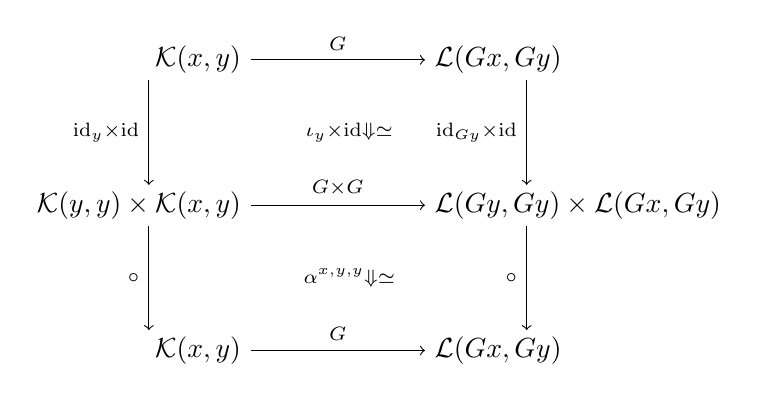
\begin{tikzpicture}[x=1.05em,y=1.05em]
  \node[anchor=east] (r1l) at (0,5) {$\mathcal{K}(x,y)$};
  \node[anchor=west] (r1r) at (6,5) {$\mathcal{L}(Gx,Gy)$};
  \node[anchor=east] (r2l) at (0,0) {$\mathcal{K}(y,y)\times\mathcal{K}(x,y)$};
  \node[anchor=west] (r2r) at (6,0) {$\mathcal{L}(Gy,Gy)\times\mathcal{L}(Gx,Gy)$};
  \node[anchor=east] (r3l) at (0,-5) {$\mathcal{K}(x,y)$};
  \node[anchor=west] (r3r) at (6,-5) {$\mathcal{L}(Gx,Gy)$};
  \draw[->] (r1l.east) -- node[above]{$\scriptstyle G$} (r1r.west);
  \draw[->] (r2l.east) -- node[above]{$\scriptstyle G{\times}G$} (r2r.west);
  \draw[->] (r3l.east) -- node[above]{$\scriptstyle G$} (r3r.west);
  \draw[->] (-3.5,4.3) -- node[left]{$\scriptstyle\mathrm{id}_{y}{\times}\mathrm{id}$} (-3.5,0.7);
  \draw[->] (9.5,4.3) -- node[left]{$\scriptstyle\mathrm{id}_{Gy}{\times}\mathrm{id}$} (9.5,0.7);
  \draw[->] (-3.5,-0.7) -- node[left]{$\scriptstyle\circ$} (-3.5,-4.3);
  \draw[->] (9.5,-0.7) -- node[left]{$\scriptstyle\circ$} (9.5,-4.3);
  \node at (3.4,2.5) {$\scriptstyle\iota_{y}{\times}\mathrm{id}\Downarrow\simeq$};
  \node at (3.4,-2.5) {$\scriptstyle\alpha^{x,y,y}\Downarrow\simeq$};
\end{tikzpicture}
\end{center}
其中这两个后者的复合均等于单位 2-\trCell{} $\mathrm{id}_{G_{x,y}}$。
\end{itemize}
\end{definition}

\begin{remark}\label{rem:terminal-qcat-notation}
为强调定义 10.4.1 与定义 10.4.4 之间的类似性，我们以 $\mathbb{1}$ 记%
\trTerminal{}\trQuasiCategory——它同时是终\trCategory{}的\trNerve；在别处，我们以 $1$ 记
一般\trInfinityCosmos{}中的\trTerminal{}∞-\trCategory。对拟范畴富集\trCategory{}中的
任意一对对象 $a$、$b\in\mathcal{L}$，有
\begin{equation*}
\Fun(\mathbb{1},\mathcal{L}(a,b))\cong\mathcal{L}(a,b),
\end{equation*}
从而 $\mathrm{h}\Fun(\mathbb{1},\mathcal{L}(a,b))\simeq\mathrm{h}\mathcal{L}(a,b)$。
于是，诸拟范畴之\trHomotopyTwoCategory{} $\mathfrak{h}\QCat$ 中以 $\mathbb{1}$ 为
定义域、以 $\mathcal{L}(a,b)$ 为余定义域的 2-\trCell{}，对应于 $\mathcal{L}$ 之%
\trHomotopyTwoCategory{}中从 $a$ 到 $b$ 的 2-\trCell{}——后者的定义与定义 1.4.1
所给者完全一致。
特别地，可逆 2-\trCell{} $\iota_{x}$ 之数据不多不少，恰是 $\mathcal{L}$ 之%
\trHomotopyTwoCategory{}中的一个可逆 2-\trCell
\begin{center}
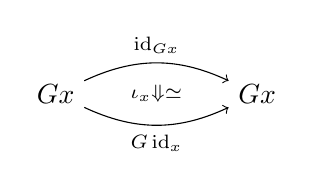
\begin{tikzpicture}[x=1.3em,y=1.3em]
  \node (l) at (-2.8,0) {$Gx$};
  \node (r) at (2.8,0) {$Gx$};
  \draw[->] (l) to[bend left=25] node[above]{$\scriptstyle\mathrm{id}_{Gx}$} (r);
  \draw[->] (l) to[bend right=25] node[below]{$\scriptstyle G\,\mathrm{id}_{x}$} (r);
  \node at (0,0) {$\scriptstyle\iota_{x}\Downarrow\simeq$};
\end{tikzpicture}
\end{center}
\end{remark}

定义 10.4.4 所引入的「拟伪函子」概念，应当被看作某个 $(\infty,2)$-范畴论概念的
2-范畴式截断，其意义如下：

\begin{digression}[拟伪函子作为 $(\infty,2)$-函子]\label{dig:quasi-pseudofunctor-infinity-2-functor}
诸拟范畴富集\trCategory{}之间的拟范畴富集\trFunctor{}可以被理解为「%
$(\infty,2)$-\trCategory{}之\trFunctor」。确实，单纯富集\trCategory{}之\trCategory{}带有
一个\trModelStructure，它呈现 $(\infty,2)$-\trCategory{}的 $(\infty,1)$-\trCategory，
其中诸\trFibrant{}对象恰是诸拟范畴富集\trCategory{} [79, 0.0.4]。然而，这一%
\trCategory{}中的诸\trFibrant{}对象未必是\trCofibrant{}的。\trCofibrant{}对象是由
Dwyer 与 Kan 最先定义的\trSimplicialComputad{} [37, 4.5]。
所以，要把一个从 $\mathcal{K}$ 到 $\mathcal{L}$ 的一般的 $(\infty,2)$-范畴论%
\trFunctor{}建模为拟范畴富集\trFunctor，必须先把 $\mathcal{K}$ 替换为一个弱等价的%
\trSimplicialComputad。
\end{digression}

这解释了为何一支\trCosmologicalBiequivalence{}之逆未必是一个严格的%
\trSimplicialFunctor，而是某种更弱的东西。列举拟范畴富集伪函子之数据的那些
2-\trCell{}相干，可以理解为「$(\infty,2)$-\trCategory{}之\trFunctor」的更高相干的
一个截断——正如诸\trQuasiCategory{}之\trHomotopyTwoCategory{}是拟范畴的拟范畴富集%
\trCategory{}的一个截断。既然本文的一个主题是：∞-范畴论的许多内容可以在截断后的%
\trHomotopyTwoCategory{}中、而非完整的 $(\infty,2)$-\trCategory{}中展开，我们便
不愿把\trCosmologicalBiequivalence{}之逆的更高相干作为定义 10.4.4 的一部分来列举。

\begin{definition}\label{def:quasi-biequivalence}
余定义域 $\mathcal{L}$ 为一个\trInfinityCosmos{}的拟伪函子
$G\colon\mathcal{K}\rightsquigarrow\mathcal{L}$，当它满足下列条件时是一个%
\textbf{\trBiequivalence}：
\begin{enumerate}[label=(\roman*)]
\item 依等价意义于对象上为满：若对一切 $a\in\mathcal{L}$ 都存在 $x\in\mathcal{K}$
使得 $Gx\simeq a$；并且
\footnote{原书印作「so that $Fx\simeq a$」，按定义头（拟伪函子记作 $G$）与本条
(ii) 之 $G_{x,y}$ 应为 $Gx$ 之误，此处径改。——译者注}
\item 诸\trQuasiCategory{}的一个\trLocalEquivalence：若对每一对 $x$、$y\in\mathcal{K}$，映射
\begin{equation*}
\mathcal{K}(x,y)\overset{G_{x,y}}{\xrightarrow{\ \sim\ }}\mathcal{L}(Gx,Gy)
\end{equation*}
是诸\trQuasiCategory{}之间的一个\trEquivalence。
\end{enumerate}
\end{definition}
\begin{remark}\label{rem:quasi-biequivalence-cosmos-codomain}
我们发现，在定义 10.4.8 中假定 $\mathcal{L}$ 是一个\trInfinityCosmos{}是方便的，
因为这使得我们得以动用定理 1.4.7 所给的 $\mathcal{L}$ 中诸\trEquivalence{}的种种
刻画。在下文中，我们要求 $\mathcal{L}$ 中的一支\trEquivalence{} $a\simeq b$：
\begin{itemize}
\item 定义 $\mathcal{L}$ 之\trHomotopyTwoCategory{}中的一个\trEquivalence；并且
\item 在诸\trQuasiCategory{}之\trHomotopyTwoCategory{}中诱导诸\trQuasiCategory{}的一个\trEquivalence{}
$\mathcal{L}(x,a)\Rightarrow\mathcal{L}(x,b)$，后者对 $x$ 是 2-自然的。
\end{itemize}
后一条性质蕴含前一条，所以，倘若我们要为一般的拟范畴富集\trCategory{}立一个
拟伪函子性\trBiequivalence{}的概念，在定义 10.4.8 中本可以采用这一\trEquivalence{}%
概念。但在诸\trInfinityCosmos{}所提供的语境之外我们并不使用这一概念，故宁取较
简单的术语。注意，我们容许定义域 $\mathcal{K}$ 仅仅是拟范畴富集的。
\end{remark}

同样地：

\begin{definition}\label{def:quasi-pseudonatural-transformation}
对诸拟范畴富集\trCategory{} $\mathcal{K}$ 与 $\mathcal{L}$ 以及拟伪函子
$F$、$G\colon\mathcal{K}\rightsquigarrow\mathcal{L}$，一个\textbf{拟范畴富集伪自然
变换}——简称\textbf{拟伪自然变换}——$\phi\colon F\Rrightarrow G$ 由如下数据给出：
\begin{itemize}
\item 对每个对象 $x\in\mathcal{K}$，一个 0-箭头 $\phi_{x}\colon Fx\to Gx\in\mathcal{L}$；
并且
\item 对每一对对象 $x$、$y\in\mathcal{K}$，在诸\trQuasiCategory{}的\trHomotopyTwoCategory{}中
的一个可逆 2-\trCell
\begin{center}
\begin{tikzpicture}[x=1.3em,y=1.3em]
  \node (tl) at (-4.2,2.2) {$\mathcal{K}(x,y)$};
  \node (tr) at (5.8,2.2) {$\mathcal{L}(Fx,Fy)$};
  \node (bl) at (-4.2,-2.2) {$\mathcal{L}(Gx,Gy)$};
  \node (br) at (5.8,-2.2) {$\mathcal{L}(Fx,Gy)$};
  \draw[->] (tl) -- node[above]{$\scriptstyle F_{x,y}$} (tr);
  \draw[->] (bl) -- node[below]{$\scriptstyle-\circ\phi_{x}$} (br);
  \draw[->] (tl) -- node[left]{$\scriptstyle G_{x,y}$} (bl);
  \draw[->] (tr) -- node[right]{$\scriptstyle\phi_{y}\circ-$} (br);
  \node at (0.6,0) {$\scriptstyle\phi^{x,y}\Downarrow\simeq$};
\end{tikzpicture}
\end{center}
\end{itemize}
使得这批数据尊重由诸拟伪函子指定的复合约束与单位约束，如下面两幅粘贴图所示：

\begin{center}
\begin{tikzpicture}[x=1em,y=1em]
  \node (A) at (0,0) {$\mathcal{K}(y,z)\times\mathcal{K}(x,y)$};
  \node (B) at (17,0) {$\mathcal{L}(Fy,Fz)\times\mathcal{L}(Fx,Fy)$};
  \node (C) at (8,-2.8) {$\mathcal{K}(x,z)$};
  \node (D) at (15.5,-2.8) {$\mathcal{L}(Fx,Fz)$};
  \node (E) at (0,-6.2) {$\mathcal{L}(Gy,Gz)\times\mathcal{L}(Gx,Gy)$};
  \node (F) at (9,-6.2) {$\mathcal{L}(Gx,Gz)$};
  \node (G) at (16,-6.2) {$\mathcal{L}(Fx,Gz)$};
  \draw[->] (A) -- node[above]{$\scriptstyle F{\times}F$} (B);
  \draw[->] (2,-0.55) -- node[above,left,pos=0.3]{$\scriptstyle\circ$} (7,-2.3);
  \node at (2.2,-1.4) {$\scriptstyle\alpha^{x,y,z}\Downarrow\simeq$};
  \draw[->] (C) -- node[above]{$\scriptstyle F$} (D);
  \draw[->] (15.5,-0.55) -- node[left,pos=0.5]{$\scriptstyle\circ$} (15.5,-2.25);
  \draw[->] (-3.5,-0.6) -- node[left]{$\scriptstyle G{\times}G$} (-3.5,-5.6);
  \node at (13.3,-1.35) {$\scriptstyle\alpha^{x,y,z}\Downarrow\simeq$};
  \draw[->] (C) -- node[left]{$\scriptstyle G$} (F);
  \draw[->] (D) -- node[right]{$\scriptstyle\phi_{z}\circ-$} (G);
  \node at (12,-4.5) {$\scriptstyle\phi^{x,z}\Downarrow\simeq$};
  \draw[->] (5.2,-6.2) -- node[above]{$\scriptstyle\circ$} (6.7,-6.2);
  \draw[->] (F) -- node[below]{$\scriptstyle-\circ\phi_{x}$} (G);
  \draw[double,double distance=1.2pt] (0,-7.1) -- (0,-7.85);
\end{tikzpicture}
\par\vspace{0.4em}
\begin{tikzpicture}[x=1em,y=1em]
  \node (A) at (0,0) {$\mathcal{K}(y,z)\times\mathcal{K}(x,y)$};
  \node (B) at (17,0) {$\mathcal{L}(Fy,Fz)\times\mathcal{L}(Fx,Fy)$};
  \node (M1) at (4,-2.9) {$\mathcal{L}(Gy,Gz)\times\mathcal{L}(Fx,Fy)$};
  \node (M2) at (17,-2.9) {$\mathcal{L}(Fy,Gz)\times\mathcal{L}(Fx,Fy)$};
  \node (E) at (-2,-6.2) {$\mathcal{L}(Gy,Gz)\times\mathcal{L}(Gx,Gy)$};
  \node (N) at (9.5,-6.2) {$\mathcal{L}(Gy,Gz)\times\mathcal{L}(Fx,Gy)$};
  \node (R) at (18.5,-6.2) {$\mathcal{L}(Fx,Gz)$};
  \draw[->] (A) -- node[above]{$\scriptstyle F{\times}F$} (B);
  \draw[->] (2,-0.55) -- node[left,pos=0.4]{$\scriptstyle G{\times}F$} (3.5,-2.35);
  \node at (10,-1.45) {$\scriptstyle\phi^{y,z}{\times}\mathrm{id}\Downarrow\simeq$};
  \draw[->] (17,-0.55) -- node[right,pos=0.5]{$\scriptstyle(\phi_{z}\circ-){\times}\mathrm{id}$} (17,-2.35);
  \draw[->] (9.3,-2.9) -- node[below]{$\scriptstyle(-\circ\phi_{y}){\times}\mathrm{id}$} (11.7,-2.9);
  \draw[->] (-5,-0.6) -- node[left]{$\scriptstyle G{\times}G$} (-5,-5.6);
  \draw[->] (1.5,-3.35) -- node[left,pos=0.6]{$\scriptstyle\mathrm{id}{\times}(\phi_{y}\circ-)$} (-1,-5.7);
  \node at (0.5,-4.6) {$\scriptstyle\mathrm{id}{\times}\phi^{x,y}\Downarrow\simeq$};
  \draw[->] (6.5,-3.35) -- node[right,pos=0.6]{$\scriptstyle\mathrm{id}{\times}(-\circ\phi_{x})$} (9,-5.7);
  \node at (12.3,-4.6) {$\scriptstyle=$};
  \draw[->] (17,-3.35) -- node[left,pos=0.5]{$\scriptstyle\circ$} (17,-5.7);
  \draw[->] (N) -- node[above]{$\scriptstyle\circ$} (R);
\end{tikzpicture}
\end{center}
\par 以及
\begin{center}
\begin{tikzpicture}[x=1.3em,y=1.3em]
  \node (1u) at (0,4.4) {$\mathbb{1}$};
  \node (tl) at (-4.6,1.8) {$\mathcal{K}(x,x)$};
  \node (tr) at (4.6,1.8) {$\mathcal{L}(Fx,Fx)$};
  \draw[->] (1u) -- node[above left]{$\scriptstyle\mathrm{id}_{x}$} (tl);
  \draw[->] (1u) -- node[above right]{$\scriptstyle\mathrm{id}_{Fx}$} (tr);
  \draw[->] (1u) -- node[left,pos=0.55]{$\scriptstyle\iota_{x}\Downarrow\simeq$} (0,2.25);
  \draw[->] (tl) -- node[above]{$\scriptstyle F_{x,x}$} (tr);
  \draw[->] (tl) -- node[left]{$\scriptstyle G_{x,x}$} (-4.6,-1.5);
  \draw[->] (tr) -- node[right]{$\scriptstyle\phi_{x}\circ-$} (4.6,-1.5);
  \node at (0,0.1) {$\scriptstyle\phi^{x,x}\Downarrow\simeq$};
  \node (bl) at (-4.6,-2.1) {$\mathcal{L}(Gx,Gx)$};
  \node (br) at (4.6,-2.1) {$\mathcal{L}(Fx,Gx)$};
  \draw[->] (bl) -- node[below]{$\scriptstyle-\circ\phi_{x}$} (br);
\end{tikzpicture}
\quad$=$\quad
\begin{tikzpicture}[x=1.3em,y=1.3em]
  \node (1u) at (0,4.4) {$\mathbb{1}$};
  \node (tl) at (-4.6,1.8) {$\mathcal{K}(x,x)$};
  \node (tr) at (4.6,1.8) {$\mathcal{L}(Gx,Gx)$};
  \draw[->] (1u) -- node[above left]{$\scriptstyle\mathrm{id}_{x}$} (tl);
  \draw[->] (1u) -- node[above right]{$\scriptstyle\mathrm{id}_{Gx}$} (tr);
  \draw[->] (1u) -- node[left,pos=0.55]{$\scriptstyle\iota_{x}\Downarrow\simeq$} (0,2.25);
  \draw[->] (tl) -- node[above]{$\scriptstyle G_{x,x}$} (tr);
  \draw[->] (tl) -- node[left]{$\scriptstyle G_{x,x}$} (-4.6,-1.8);
  \draw[->] (tr) -- node[right]{$\scriptstyle-\circ\phi_{x}$} (4.6,-1.8);
  \node (bl) at (-4.6,-2.1) {$\mathcal{L}(Gx,Gx)$};
  \node (br) at (4.6,-2.1) {$\mathcal{L}(Fx,Gx)$};
  \draw[->] (bl) -- node[below]{$\scriptstyle-\circ\phi_{x}$} (br);
\end{tikzpicture}
\end{center}
\footnote{左图之中部 2-胞腔原书印作「$\phi^{x,y}\Downarrow\simeq$」，然图中仅涉
对象 $x$，应为 $\phi^{x,x}$ 之误，此处径改。——译者注}
\end{definition}

\begin{remark}\label{rem:analogy-pseudonatural-quasi}
定义 10.4.2 与定义 10.4.10 之间的类似性，平行于定义 10.4.1 与定义 10.4.4 之间的
类似性——只是这层类似被我们的陈述方式遮蔽了。伪函子 $F$、$G\colon\mathcal{C}\rightsquigarrow\mathcal{D}$
之间的伪自然变换 $\phi\colon F\Rrightarrow G$ 之可逆 2-\trCell{}分量的自然性要求告诉我们：
它们可以装配成\trFunctor{}之间的一个自然同构
\begin{center}
\begin{tikzpicture}[x=1.3em,y=1.3em]
  \node (tl) at (-4.2,2.2) {$\mathcal{C}(x,y)$};
  \node (tr) at (5.4,2.2) {$\mathcal{D}(Fx,Fy)$};
  \node (bl) at (-4.2,-2.2) {$\mathcal{D}(Gx,Gy)$};
  \node (br) at (5.4,-2.2) {$\mathcal{D}(Fx,Gy)$};
  \draw[->] (tl) -- node[above]{$\scriptstyle F_{x,y}$} (tr);
  \draw[->] (bl) -- node[below]{$\scriptstyle-\circ\phi_{x}$} (br);
  \draw[->] (tl) -- node[left]{$\scriptstyle G_{x,y}$} (bl);
  \draw[->] (tr) -- node[right]{$\scriptstyle\phi_{y}\circ-$} (br);
  \node at (0.6,0) {$\scriptstyle\phi^{x,y}\Downarrow\simeq$};
\end{tikzpicture}
\end{center}
对每一对 $x$、$y\in\mathcal{C}$ 成立。表达这些自然同构与复合约束及单位约束相容的
诸相干条件，随后可以写成定义 10.4.10 中出现的那种形式；但由于两个自然同构相等，
当且仅当它们的分量相等，我们可以把这些相干条件化归为定义 10.4.2 的其余两条粘贴
等式——用 $\phi$ 的分量表出。

\trQuasiCategory{}之间的\trFunctor{}之间的自然同构，其数据比\trCategory{}之间的\trFunctor{}之间
的自然同构更为错综；这正是定义 10.4.10 的诸相干条件必须以更普遍的方式表出的原因。不过，定义 10.4.2 的诸相干条件可以从这些条件中如下抽取出来。

请回忆：$\mathcal{K}(x,y)$ 中的 0-箭头对应于\trFunctor{}
$f\colon\mathbb{1}\to\mathcal{K}(x,y)$。由\cref{rem:terminal-qcat-notation}，限制
$\phi^{x,y}f$ 定义了 $\mathfrak{h}\mathcal{L}$ 中一个可逆 2-\trCell{}的分量
\begin{center}
\begin{tikzpicture}[x=1.3em,y=1.3em]
  \node (tl) at (-3.2,2) {$Fx$};
  \node (tr) at (3.2,2) {$Fy$};
  \node (bl) at (-3.2,-2) {$Gx$};
  \node (br) at (3.2,-2) {$Gy$};
  \draw[->] (tl) -- node[above]{$\scriptstyle Ff$} (tr);
  \draw[->] (bl) -- node[below]{$\scriptstyle Gf$} (br);
  \draw[->] (tl) -- node[left]{$\scriptstyle\phi_{x}$} (bl);
  \draw[->] (tr) -- node[right]{$\scriptstyle\phi_{y}$} (br);
  \node at (0,0) {$\scriptstyle\phi_{f}\Downarrow\simeq$};
\end{tikzpicture}
\end{center}
这一 2-\trCell{}自动是自然的，其意义为：对 $\mathcal{K}$ 的\trHomotopyTwoCategory{}中的
每个 2-\trCell{}
\begin{tikzpicture}[x=1em,y=0.9em,baseline=-0.5em]
  \node (x) at (0,0) {$x$};
  \node (y) at (4.2,0) {$y$};
  \draw[->] (0.5,0.35) to[bend left=25] (3.7,0.35);
  \node at (2.1,1.35) {$\scriptstyle f$};
  \draw[->] (3.7,-0.35) to[bend left=25] (0.5,-0.35);
  \node at (2.1,-1.35) {$\scriptstyle g$};
  \node at (2.1,0) {$\scriptstyle\Downarrow\gamma$};
\end{tikzpicture}，
粘贴复合
\begin{center}
\begin{tikzpicture}[x=1.3em,y=1.3em]
  \node (tl) at (-3.4,3.2) {$Fx$};
  \node (tr) at (3.4,3.2) {$Fy$};
  \node (bl) at (-3.4,-3.2) {$Gx$};
  \node (br) at (3.4,-3.2) {$Gy$};
  \draw[->] (tl) to[bend left=20] node[above]{$\scriptstyle Ff$} (tr);
  \draw[->] (tl) to[bend left=6] node[above,pos=0.72]{$\scriptstyle Fg$} (tr);
  \node at (0.2,1.45) {$\scriptstyle\Downarrow F\gamma$};
  \draw[->] (tl) -- node[left]{$\scriptstyle\phi_{x}$} (bl);
  \draw[->] (tr) -- node[right]{$\scriptstyle\phi_{y}$} (br);
  \node at (0,-1.5) {$\scriptstyle\phi_{g}\Downarrow\simeq$};
  \draw[->] (bl) to[bend right=20] node[below]{$\scriptstyle Gg$} (br);
\end{tikzpicture}
\quad$=$\quad
\begin{tikzpicture}[x=1.3em,y=1.3em]
  \node (tl) at (-3.4,3.2) {$Fx$};
  \node (tr) at (3.4,3.2) {$Fy$};
  \node (bl) at (-3.4,-3.2) {$Gx$};
  \node (br) at (3.4,-3.2) {$Gy$};
  \draw[->] (tl) to[bend left=20] node[above]{$\scriptstyle Ff$} (tr);
  \node at (0,1.5) {$\scriptstyle\phi_{f}\Downarrow\simeq$};
  \draw[->] (tl) -- node[left]{$\scriptstyle\phi_{x}$} (bl);
  \draw[->] (tr) -- node[right]{$\scriptstyle\phi_{y}$} (br);
  \draw[->] (bl) to[bend left=8] node[above,pos=0.3]{$\scriptstyle Gf$} (br);
  \node at (0.2,-1.6) {$\scriptstyle\Downarrow G\gamma$};
  \draw[->] (bl) to[bend right=20] node[below]{$\scriptstyle Gg$} (br);
\end{tikzpicture}
\end{center}
在 $\mathcal{L}$ 的\trHomotopyTwoCategory{}中相等。这由须状复合的自然性（见附录 B 中的%
\cref{lem:naturality-of-whiskering}）
得出，因为两个粘贴复合都由诸\trQuasiCategory{}的\trHomotopyTwoCategory{}中的如下水平复合
\begin{center}
\begin{tikzpicture}[x=1.3em,y=1.3em]
  \node (1u) at (0,0) {$\mathbb{1}$};
  \node (K) at (5.6,0) {$\mathcal{K}(x,y)$};
  \node (L) at (14.5,0) {$\mathcal{L}(Fx,Gy)$};
  \draw[->] (1u) to[bend left=25] node[above]{$\scriptstyle f$} (K);
  \draw[->] (1u) to[bend right=25] node[below]{$\scriptstyle g$} (K);
  \node at (2.5,0) {$\scriptstyle\Downarrow\gamma$};
  \draw[->] (K) -- (L);
  \node at (10.05,0.9) {$\scriptstyle(\phi_{y}\circ-)\circ F_{x,y}$};
  \node at (10.05,0.12) {$\scriptstyle\phi^{x,y}\Downarrow\simeq$};
  \node at (10.05,-0.85) {$\scriptstyle(-\circ\phi_{x})\circ G_{x,y}$};
\end{tikzpicture}
\end{center}
所表示。

类似地，定义 10.4.10 的复合图表与单位图表蕴含：定义 10.4.2 中所展示的相应图表在
$\mathcal{L}$ 的\trHomotopyTwoCategory{}中交换（见\cref{ex:pasting-equalities-quasi}）。
\end{remark}

对任意拟范畴富集\trCategory{} $\mathcal{K}$，hom-\trBifunctor{}
$\mathcal{K}(-,-)\colon\mathcal{K}^{\mathrm{op}}\times\mathcal{K}\to\QCat{}$ 是一个
拟范畴富集\trFunctor。

\begin{lemma}\label{lem:action-on-homs-qpn}
拟伪函子 $F\colon\mathcal{K}\rightsquigarrow\mathcal{L}$（介于诸拟范畴富集%
\trCategory{} $\mathcal{K}$ 与 $\mathcal{L}$ 之间）在 hom 上的作用，定义了一个拟伪
自然变换
\begin{equation*}
F_{-,-}\colon\mathcal{K}(-,-)\Rrightarrow\mathcal{L}(F-,F-)
\end{equation*}
介于拟伪自然函子 $\mathcal{K}^{\mathrm{op}}\times\mathcal{K}\rightsquigarrow\QCat{}$
之间。
\footnote{此处「拟伪自然函子」照录原书面貌（quasi-pseudonatural
functors）；按上下文（前段已证 $\mathcal{K}(-,-)$ 为拟范畴富集\trFunctor）疑为
「拟范畴富集函子」（quasi-categorically enriched functors）之误。——译者注}
\end{lemma}

\begin{proof}
与 $\mathcal{K}^{\mathrm{op}}\times\mathcal{K}$ 中一对对象 $(x,y)$ 与 $(w,z)$ 相关联
的该拟伪自然变换之 2-\trCell{}分量为
\begin{center}
\begin{tikzpicture}[x=1.3em,y=1.3em]
  \node (tl) at (-4.6,2.2) {$\mathcal{K}(y,z)\times\mathcal{K}(w,x)$};
  \node (tr) at (5.6,2.2) {$\mathcal{K}(w,z)^{\mathcal{K}(x,y)}$};
  \node (bl) at (-4.6,-2.2) {$\mathcal{L}(Fw,Fz)^{\mathcal{L}(Fx,Fy)}$};
  \node (br) at (5.6,-2.2) {$\mathcal{L}(Fw,Fz)^{\mathcal{K}(x,y)}$};
  \draw[->] (tl) -- node[above]{$\scriptstyle\circ$} (tr);
  \draw[->] (bl) -- node[below]{$\scriptstyle-\circ F_{x,y}$} (br);
  \draw[->] (tl) -- node[left]{$\scriptstyle F$} (bl);
  \draw[->] (tr) -- node[right]{$\scriptstyle F_{w,z}\circ-$} (br);
  \node at (0.5,0) {$\scriptstyle\alpha^{w,x,y,z}\Downarrow\simeq$};
\end{tikzpicture}
\end{center}
其中 $\alpha^{w,x,y,z}$ 是 \eqref{eq:quasi-pseudofunctor-pasting} 所定义的公共
2-\trCell{}的一个转置。复合公理与单位公理的验证留给\cref{ex:finish-lemma-proof}。
\end{proof}

\begin{definition}\label{def:quasi-pseudonatural-equivalence}
余定义域为一个\trInfinityCosmos{}的、拟伪函子 $F$、$G\colon\mathcal{K}\rightsquigarrow\mathcal{L}$
之间的拟伪自然变换 $\phi\colon F\Rrightarrow G$，若其每个分量
$\phi_{x}\colon Fx\to Gx$ 都定义 $\mathcal{L}$ 的\trHomotopyTwoCategory{}中的一个%
\trEquivalence，便是一个\textbf{拟伪自然等价}。
\end{definition}

由于\cref{rem:quasi-biequivalence-cosmos-codomain}中所述的理由，假定 $\mathcal{L}$
是一个\trInfinityCosmos{}是方便的，这样我们便无须对目标\trCategory{}中\trEquivalence{}的
恰当概念作进一步的明确。我们对拟伪自然等价这一类的兴趣源于下述结果——它可以理解
为\trBicategory{} \trYonedaLemma{}在拟范畴富集\trCategory、拟伪函子与拟伪自然变换之语境中的
一个版本。

\begin{lemma}\label{lem:quasi-yoneda}
若在\trInfinityCosmos{} $\mathcal{K}$ 中由一对对象 $a$、$b$ 所\trRepresentable{}%
诸\trSimplicialFunctor{} $\mathcal{K}^{\mathrm{op}}\to\QCat{}$ 之间存在一条拟伪自然
等价
\begin{equation*}
\phi\colon\mathcal{K}(-,a)\Rrightarrow\mathcal{K}(-,b)
\end{equation*}
则 $a$ 与 $b$ 在 $\mathcal{K}$ 中等价。
\end{lemma}

\begin{proof}
我们将证明：0-箭头 $y\coloneqq\phi_{a}(\mathrm{id}_{a})\colon a\to b$ 是 $\mathcal{K}$
中的一个\trEquivalence。首先观察到：对每个 $x\in\mathcal{K}$，分量
$\phi_{x}\colon\mathcal{K}(x,a)\Rightarrow\mathcal{K}(x,b)$——下图中的右上复合——
在诸\trQuasiCategory{}的\trHomotopyTwoCategory{}中同构于经 $y$ 的后复合——即
下图中的左下复合：
\begin{center}
\begin{tikzpicture}[x=1.3em,y=1.3em]
  \node (P1) at (0,0) {$\mathcal{K}(x,a)$};
  \node (P2) at (10.5,0) {$\mathcal{K}(x,a)^{\mathcal{K}(a,a)}$};
  \node (P3) at (0,-4.2) {$\mathcal{K}(x,b)^{\mathcal{K}(a,b)}$};
  \node (P4) at (10.5,-4.2) {$\mathcal{K}(x,b)^{\mathcal{K}(a,a)}$};
  \node (P5) at (18,-1.6) {$\mathcal{K}(x,a)$};
  \node (P6) at (18,-4.2) {$\mathcal{K}(x,b)$};
  \node (P7) at (7.5,-7) {$\mathcal{K}(x,b)$};
  \node (P8) at (13,-7) {$\mathcal{K}(x,b)$};
  \draw[->] (P1) -- node[above]{$\scriptstyle\circ$} (P2);
  \draw[->] (P1) -- node[left]{$\scriptstyle\circ$} (P3);
  \node at (2.9,-2.1) {$\scriptstyle\phi^{x,a}\Downarrow\simeq$};
  \draw[->] (P2) -- node[right]{$\scriptstyle\phi_{x}\circ-$} (P4);
  \draw[->] (P3) -- node[below]{$\scriptstyle-\circ\phi_{a}$} (P4);
  \draw[->] (P4) -- node[below]{$\scriptstyle\mathrm{ev}_{\mathrm{id}_{a}}$} (P6);
  \draw[->] (P2) -- node[above right]{$\scriptstyle\mathrm{ev}_{\mathrm{id}_{a}}$} (P5);
  \draw[->] (P5) -- node[right]{$\scriptstyle\phi_{x}$} (P6);
  \draw[->] (P3) -- node[below left]{$\scriptstyle\mathrm{ev}_{y}$} (P7);
  \draw[double,double distance=1.2pt] (P7) -- (P8);
\end{tikzpicture}
\quad$\eqqcolon$\quad
\begin{tikzpicture}[x=1.3em,y=1.3em]
  \node (l) at (0,0) {$\mathcal{K}(x,a)$};
  \node (r) at (5.6,0) {$\mathcal{K}(x,b)$};
  \draw[->] (l) to[bend left=25] node[above]{$\scriptstyle\phi_{x}$} (r);
  \draw[->] (l) to[bend right=25] node[below]{$\scriptstyle y\circ-$} (r);
  \node at (2.8,0) {$\scriptstyle\Downarrow\simeq$};
\end{tikzpicture}
\end{center}
特别地，由练习 1.4.iii，映射 $y\circ-\colon\mathcal{K}(x,a)\Rightarrow\mathcal{K}(x,b)$
对任何 $x\in\mathcal{K}$ 都是一个\trEquivalence，这意味着
$y\colon a\Rightarrow b$ 是\trInfinityCosmos{} $\mathcal{K}$ 中的一个%
\trEquivalence。
\end{proof}

拟伪自然等价可以构造为：逐分量定义\trEquivalence{}的那些\trSimplicial{}自然变换之
伴随等价逆。

\begin{lemma}\label{lem:adjoint-inverses-qpn}
考虑∞-宇宙间的拟范畴富集\trFunctor{}间的\trSimplicial{}自然变换
\begin{tikzpicture}[x=1em,y=0.9em,baseline=-0.5em]
  \node (K) at (0,0) {$\mathcal{K}$};
  \node (L) at (4.6,0) {$\mathcal{L}$};
  \draw[->] (0.5,0.4) to[bend left=25] (4.1,0.4);
  \node at (2.3,1.35) {$\scriptstyle F$};
  \node at (2.3,0) {$\scriptstyle\Downarrow\phi$};
  \draw[->] (4.1,-0.4) to[bend left=25] (0.5,-0.4);
  \node at (2.3,-1.35) {$\scriptstyle G$};
\end{tikzpicture}，
其中 0-箭头分量 $\phi_{x}\colon Fx\Rightarrow Gx$ 全都定义 $\mathcal{L}$ 中的%
\trEquivalence。则伴随等价逆 $\psi_{x}\colon Gx\Rightarrow Fx$ 的任何选取都可装配成一条
拟伪自然变换 $\psi\colon G\Rrightarrow F$ 的诸分量，后者是一个拟伪自然等价。
\end{lemma}

\begin{proof}
拟伪自然变换 $\psi$ 的诸分量由伴随等价逆箭头 $\psi_{x}\colon Gx\Rightarrow Fx$ 与下述粘贴
复合自然变换定义
\begin{center}
\begin{tikzpicture}[x=1.3em,y=1.3em]
  \node (Q1) at (0,0) {$\mathcal{K}(x,y)$};
  \node (Q2) at (10.5,0) {$\mathcal{L}(Gx,Gy)$};
  \node (Q3) at (0,-4.2) {$\mathcal{L}(Fx,Fy)$};
  \node (Q4) at (7.2,-4.2) {$\mathcal{L}(Fx,Gy)$};
  \node (Q5) at (14.8,-4.2) {$\mathcal{L}(Gx,Gy)$};
  \node (Q6) at (6.2,-7.6) {$\mathcal{L}(Fx,Fy)$};
  \node (Q7) at (14.8,-7.6) {$\mathcal{L}(Gx,Fy)$};
  \node at (-5.4,-2.1) {$\psi^{x,y}\coloneqq$};
  \draw[->] (Q1) -- node[above]{$\scriptstyle G_{x,y}$} (Q2);
  \draw[->] (Q1) -- node[left]{$\scriptstyle F_{x,y}$} (Q3);
  \draw[->] (Q2) -- node[left,pos=0.6]{$\scriptstyle-\circ\phi_{x}$} (Q4);
  \draw[double,double distance=1.6pt] (Q2) -- node[above right,pos=0.45]{$\scriptstyle\eta_{x}\simeq$} (Q5);
  \draw[->] (Q3) -- node[above,pos=0.55]{$\scriptstyle\phi_{y}\circ-$} (Q4);
  \draw[->] (Q4) -- node[above]{$\scriptstyle-\circ\psi_{x}$} (Q5);
  \draw[->] (Q4) -- node[left,pos=0.5]{$\scriptstyle\psi_{y}\circ-$} (Q7);
  \draw[->] (Q5) -- node[right]{$\scriptstyle\psi_{y}\circ-$} (Q7);
  \draw[double,double distance=1.6pt] (Q3) -- node[below left,pos=0.5]{$\scriptstyle\epsilon_{y}\simeq$} (Q6);
  \draw[->] (Q6) -- node[below]{$\scriptstyle-\circ\psi_{x}$} (Q7);
\end{tikzpicture}
\end{center}
涉及该伴随等价的单位同构与余单位同构。

由于 $F$ 与 $G$ 是\trSimplicialFunctor，单位条件化简为只要求：这一粘贴自然变换在
恒同箭头 $\mathrm{id}_{x}\colon\mathbb{1}\to\mathcal{K}(x,x)$ 处的分量是一个恒同
2-\trCell{} $\mathrm{id}_{\psi_{x}}$。这一分量是粘贴复合
\begin{center}
\begin{tikzpicture}[x=1.3em,y=1.3em]
  \node (A) at (-2.8,1.7) {$Gx$};
  \node (B) at (2.8,1.7) {$Gx$};
  \node (C) at (-2.8,-1.7) {$Fx$};
  \node (D) at (2.8,-1.7) {$Fx$};
  \draw[double,double distance=1.2pt] (A) -- (B);
  \draw[double,double distance=1.2pt] (C) -- (D);
  \draw[->] (A) -- node[left]{$\scriptstyle\psi_{x}$} (C);
  \draw[->] (B) -- node[right]{$\scriptstyle\psi_{x}$} (D);
  \draw[->] (C) to[bend left=20] node[left,pos=0.6]{$\scriptstyle\phi_{x}$} (B);
  \node at (0,1.05) {$\scriptstyle\eta\simeq$};
  \node at (-0.4,-1.05) {$\scriptstyle\epsilon\simeq$};
\end{tikzpicture}
\end{center}
由于所指定的数据定义一个伴随等价，这确为恒同。

类似地，为验证复合公理，我们必须证明复合
\begin{center}
\begin{tikzpicture}[x=1.3em,y=1.3em]
  \node (V1) at (0,2) {$\mathcal{K}(y,z)\times\mathcal{K}(x,y)$};
  \node (V2) at (7,0.3) {$\mathcal{K}(x,z)$};
  \node (V3) at (14.5,0.3) {$\mathcal{L}(Gx,Gz)$};
  \node (V4) at (0,-3.4) {$\mathcal{L}(Fx,Fz)$};
  \node (V5) at (9.5,-3.4) {$\mathcal{L}(Fx,Gz)$};
  \node (V6) at (17.5,-3.4) {$\mathcal{L}(Gx,Gz)$};
  \node (V7) at (4,-7) {$\mathcal{L}(Fx,Fz)$};
  \node (V8) at (13,-7) {$\mathcal{L}(Gx,Fz)$};
  \draw[->] (V1) -- node[above,left,pos=0.55]{$\scriptstyle\circ$} (V2);
  \draw[->] (V2) -- node[above]{$\scriptstyle G_{x,z}$} (V3);
  \draw[->] (V2) -- node[left,pos=0.6]{$\scriptstyle F_{x,z}$} (V4);
  \draw[->] (V3) -- node[left]{$\scriptstyle-\circ\phi_{x}$} (V5);
  \draw[double,double distance=1.6pt] (V3) -- node[above right,pos=0.5]{$\scriptstyle\eta_{x}\simeq$} (V6);
  \draw[->] (V4) -- node[above]{$\scriptstyle\phi_{z}\circ-$} (V5);
  \draw[->] (V5) -- node[above]{$\scriptstyle-\circ\psi_{x}$} (V6);
  \draw[double,double distance=1.6pt] (V4) -- node[left,pos=0.5]{$\scriptstyle\epsilon_{z}\simeq$} (V7);
  \draw[->] (V5) -- node[left]{$\scriptstyle\psi_{z}\circ-$} (V7);
  \draw[->] (V6) -- node[right]{$\scriptstyle\psi_{z}\circ-$} (V8);
  \draw[->] (V7) -- node[below]{$\scriptstyle-\circ\psi_{x}$} (V8);
\end{tikzpicture}
\end{center}
等于
\begin{center}
\begin{tikzpicture}[x=1.15em,y=1.15em]
  \node (K) at (10.5,0) {$\mathcal{K}(y,z){\times}\mathcal{K}(x,y)$};
  \node (L2) at (0,-3.2) {$\mathcal{L}(Fy,Fz){\times}\mathcal{L}(Fx,Fy)$};
  \node (M2) at (10.5,-3.2) {$\mathcal{L}(Fy,Fz){\times}\mathcal{L}(Gx,Gy)$};
  \node (R2) at (21,-3.2) {$\mathcal{L}(Gy,Gz){\times}\mathcal{L}(Gx,Gy)$};
  \node (L3) at (5,-6.6) {$\mathcal{L}(Fy,Fz){\times}\mathcal{L}(Fx,Gy)$};
  \node (M3) at (15,-6.6) {$\mathcal{L}(Fy,Gz){\times}\mathcal{L}(Gx,Gy)$};
  \node (L4) at (0,-10.2) {$\mathcal{L}(Fy,Fz){\times}\mathcal{L}(Fx,Fy)$};
  \node (M4) at (10.5,-10.2) {$\mathcal{L}(Fy,Fz){\times}\mathcal{L}(Gx,Gz)$};
  \node (L5) at (5,-13.8) {$\mathcal{L}(Fy,Fz){\times}\mathcal{L}(Gx,Fy)$};
  \node (R5) at (16,-13.8) {$\mathcal{L}(Gy,Fz){\times}\mathcal{L}(Gx,Gy)$};
  \node (R2p) at (21,-10.2) {$\mathcal{L}(Gy,Gz){\times}\mathcal{L}(Gx,Gy)$};
  \node (Z) at (10.5,-17.4) {$\mathcal{L}(Gx,Fz)$};
  \draw[->] (K) -- node[above,left,pos=0.6]{$\scriptstyle F{\times}F$} (L2);
  \draw[->] (K) -- node[left]{$\scriptstyle F{\times}G$} (M2);
  \draw[->] (K) -- node[above,right,pos=0.6]{$\scriptstyle G{\times}G$} (R2);
  \draw[->] (L2) -- node[left,pos=0.5]{$\scriptstyle\phi_{y}\circ-$} (L3);
  \draw[->] (M2) -- node[above,pos=0.4]{$\scriptstyle-\circ\phi_{x}$} (L3);
  \draw[->] (13.2,-3.55) -- node[right,pos=0.4]{$\scriptstyle\phi_{z}\circ-$} (15.4,-6.25);
  \draw[double,double distance=1.4pt] (M2) -- (M4);
  \node at (12.1,-5.1) {$\scriptstyle\epsilon_{z}\simeq$};
  \node at (9.0,-8.9) {$\scriptstyle\eta_{x}\simeq$};
  \draw[->] (R2) -- node[right,pos=0.35]{$\scriptstyle-\circ\phi_{y}$} (M3);
  \draw[->] (L3) -- node[left]{$\scriptstyle\psi_{y}\circ-$} (L4);
  \draw[->] (L3) -- node[above,pos=0.35]{$\scriptstyle-\circ\psi_{x}$} (M4);
  \draw[->] (M3) -- node[above,pos=0.5]{$\scriptstyle-\circ\psi_{y}$} (R2p);
  \draw[double,double distance=1.6pt] (L2) to[bend right=30] node[left,pos=0.5]{$\scriptstyle\epsilon_{y}\simeq$} (L4);
  \draw[double,double distance=1.6pt] (R2) to[bend left=30] node[right,pos=0.45]{$\scriptstyle\eta_{y}\simeq$} (R2p);
  \draw[->] (L4) -- node[below,pos=0.4]{$\scriptstyle-\circ\psi_{x}$} (L5);
  \draw[->] (M4) -- node[left,pos=0.5]{$\scriptstyle\psi_{y}\circ-$} (L5);
  \draw[->] (M4) -- node[above,pos=0.45]{$\scriptstyle-\circ\psi_{y}$} (R5);
  \draw[->] (R2.south) to[bend left=15] node[right,pos=0.75]{$\scriptstyle\psi_{z}\circ-$} (R5);
  \draw[->] (R2p) -- node[right,pos=0.4]{$\scriptstyle\psi_{z}\circ-$} (R5);
  \draw[->] (L5) -- node[above,left]{$\scriptstyle\circ$} (Z);
  \draw[->] (R5) -- node[above,right]{$\scriptstyle\circ$} (Z);
\end{tikzpicture}
\end{center}
图中出现的\trPreComposition{}映射与\trPostComposition{}映射都是 2-自然的（见定义 B.2.2），因此例如
$\epsilon_{y}$ 与 $-\circ\psi_{x}$ 的须状复合可以按任意一次序构成。在第二幅粘贴图
中反复使用这条交换性质，并运用三角等式
$\phi_{y}\epsilon_{y}\cdot\eta_{y}\phi_{y}=\mathrm{id}_{\phi_{y}}$，第二幅粘贴图便
化归为第一幅。
\end{proof}

现在我们证明：诸\trInfinityCosmos{}之间的任何一支\trBiequivalence{}
$F\colon\mathcal{K}\Rightarrow\mathcal{L}$ 都容许一个拟伪函子性的「逆」
$G\colon\mathcal{L}\rightsquigarrow\mathcal{K}$，并配备拟伪自然等价
$\eta\colon\mathrm{id}_{\mathcal{K}}\Rrightarrow GF$ 与
$\epsilon\colon FG\Rrightarrow\mathrm{id}_{\mathcal{L}}$。

\begin{proposition}\label{prop:quasi-pseudoinverse}
若 $F\colon\mathcal{K}\to\mathcal{L}$ 是诸\trInfinityCosmos{}之间的一个拟范畴
富集\trFunctor{}兼\trBiequivalence，则存在一个拟伪函子
$G\colon\mathcal{L}\rightsquigarrow\mathcal{K}$，它也是一支\trBiequivalence。而且，
$G$ 是 $F$ 的一个\emph{拟伪逆}，其意义为：存在拟伪自然等价
$\mathrm{id}_{\mathcal{K}}\Rrightarrow GF$ 与 $FG\Rrightarrow\mathrm{id}_{\mathcal{L}}$。
\end{proposition}

\begin{proof}
为融贯地定义\trBiequivalence{} $F\colon\mathcal{K}\Rightarrow\mathcal{L}$ 的一支逆，
我们「完整指定」其数据，选取：
\begin{itemize}
\item[($\beta$)] 对每个 $a\in\mathcal{L}$，完整指定的伴随等价
$\epsilon_{a}\colon Fx_{a}\simeq a$；并且
\item[($\gamma$)] 对每一对 $x$、$y\in\mathcal{K}$，完整指定的、诸拟范畴之伴随等价的逆
\begin{equation*}
\mathcal{K}(x,y)\xrightarrow[\ \sim\ ]{F_{x,y}}\mathcal{L}(Fx,Fy)
\end{equation*}
其逆对 $x$ 与 $y$ 是拟伪自然的。
\end{itemize}
在 ($\gamma$) 中，我们将\cref{lem:adjoint-inverses-qpn}应用于\trSimplicial{}自然变换
$F_{-,-}\colon\mathcal{K}(-,-)\to\mathcal{L}(F-,F-)$，从而观察到：对这些映射逐点取的
伴随等价可装配成一个拟伪自然变换，而且后者还是一个逐点等价。
\footnote{原书印作「In $(\gamma)$, we apply to the simplicial natural
transformation $F_{-,-}\colon\mathcal{K}(-,-)\to\mathcal{L}(F-,F-)$ to
observe…」，apply 之后疑脱漏所引条目名；按文义（伴随等价逆装配成拟伪自然变换）
应为引理 10.4.15，据文义补。——译者注}

现在，为定义 $G\colon\mathcal{L}\rightsquigarrow\mathcal{K}$，用 ($\beta$) 为每个
$a\in\mathcal{L}$ 指定一个对象 $Ga\coloneqq x_{a}\in\mathcal{K}$，连同一支\trEquivalence{}
$\epsilon_{a}\colon FGa\simeq a$（在 $\mathcal{L}$ 中）。这就定义了 $G$ 在对象上的
映射以及拟伪自然变换 $\epsilon$ 的 0-箭头分量。为定义 $G$ 在诸\trFunctorSpace{}上的
作用，用这批数据与 ($\gamma$) 定义
\begin{equation*}
G_{a,b}\coloneqq\mathcal{L}(a,b)
\xrightarrow[\ \sim\ ]{\ (-\circ\epsilon_{a},\,\epsilon_{b}^{-1}\circ-)\ }
\mathcal{L}(FGa,FGb)
\xrightarrow[\ \sim\ ]{\ F_{Ga,Gb}^{-1}\ }
\mathcal{K}(Ga,Gb)
\end{equation*}

对每个 $a\in\mathcal{L}$，定义 $\iota_{a}\colon\mathrm{id}_{Ga}\cong G_{a,a}\,\mathrm{id}_{a}$
为下述复合
\begin{center}
\begin{tikzpicture}[x=1.3em,y=1.3em]
  \node (1u) at (0,2.6) {$\mathbb{1}$};
  \node (l) at (-8.2,0) {$\mathcal{L}(a,a)$};
  \node (m) at (0.4,0) {$\mathcal{L}(FGa,FGa)$};
  \node (r) at (8.6,0) {$\mathcal{K}(Ga,Ga)$};
  \draw[->] (1u) -- node[above left]{$\scriptstyle\mathrm{id}_{a}$} (l);
  \draw[->] (1u) -- node[above right]{$\scriptstyle\mathrm{id}_{Ga}$} (r);
  \draw[->] (1u) -- node[right,pos=0.5]{$\scriptstyle\mathrm{id}_{FGa}$} (m);
  \node at (-3.9,0.45) {$\scriptstyle\beta\simeq$};
  \node at (4.5,0.45) {$\scriptstyle\gamma\simeq$};
  \draw[->] (l) -- node[above]{$\scriptstyle\simeq$}
    node[below]{$\scriptstyle(-\circ\epsilon_{a},\,\epsilon_{a}^{-1}\circ-)$} (m);
  \draw[->] (m) -- node[above]{$\scriptstyle\simeq$}
    node[below]{$\scriptstyle F_{Ga,Ga}^{-1}$} (r);
\end{tikzpicture}
\end{center}
即把 $\mathfrak{h}\mathcal{L}$ 中的\trIsomorphism{}
$\beta_{a}\colon\epsilon_{a}^{-1}\circ\epsilon_{a}\cong\mathrm{id}_{FGa}$ 与%
\trIsomorphism{}
$\gamma\colon F_{Ga,Ga}^{-1}\circ F_{Ga,Ga}\cong\mathrm{id}_{\mathcal{K}(Ga,Ga)}$ 在
$\mathrm{id}_{Ga}$ 处的分量。对每个 $a$、$b$、$c\in\mathcal{L}$，定义 $\alpha^{a,b,c}$
为由 ($\beta$) 与 ($\gamma$) 之数据构造的诸典范\trNaturalTransformation{}的如下复合
\begin{center}
\begin{tikzpicture}[x=1.3em,y=1.3em]
  \node (W1) at (0,2.4) {$\mathcal{L}(b,c)\times\mathcal{L}(a,b)$};
  \node (W2) at (9.5,2.4) {$\mathcal{L}(a,c)$};
  \node (X1) at (0,0) {$\mathcal{L}(FGb,FGc)\times\mathcal{L}(FGa,FGb)$};
  \node (X2) at (9.5,0) {$\mathcal{L}(FGa,FGc)$};
  \node (Y1) at (0,-2.4) {$\mathcal{K}(Gb,Gc)\times\mathcal{K}(Ga,Gb)$};
  \node (Y2) at (9.5,-2.4) {$\mathcal{K}(Ga,Gc)$};
  \draw[->] (W1) -- node[above]{$\scriptstyle\circ$} (W2);
  \draw[->] (X1) -- node[above]{$\scriptstyle\circ$} (X2);
  \draw[->] (Y1) -- node[above]{$\scriptstyle\circ$} (Y2);
  \draw[->] (W1) -- node[left]{$\scriptstyle(-\circ\epsilon_{b},\epsilon_{c}^{-1}\circ-)\times(-\circ\epsilon_{a},\epsilon_{b}^{-1}\circ-)$} (X1);
  \draw[->] (W2) -- node[right]{$\scriptstyle(-\circ\epsilon_{a},\epsilon_{c}^{-1}\circ-)$} (X2);
  \node at (5.4,1.2) {$\scriptstyle\beta\simeq$};
  \draw[->] (X1) -- node[left]{$\scriptstyle F_{Gb,Gc}^{-1}{\times}F_{Ga,Gb}^{-1}$} (Y1);
  \draw[->] (X2) -- node[right]{$\scriptstyle F_{Ga,Gc}^{-1}$} (Y2);
  \node at (5.4,-1.2) {$\scriptstyle\gamma\simeq$};
\end{tikzpicture}
\end{center}

我们接着验证：这些选取使 $G$ 成为一个拟伪函子。为单位条件，我们必须验证复合
\begin{center}
\begin{tikzpicture}[x=1.1em,y=1.6em]
  \node (U11) at (0,2.4) {$\mathcal{L}(a,b)$};
  \node (U12) at (10,2.4) {$\mathcal{L}(b,b)\times\mathcal{L}(a,b)$};
  \node (U13) at (21,2.4) {$\mathcal{L}(a,b)$};
  \node (U21) at (0,0) {$\mathcal{L}(FGa,FGb)$};
  \node (U22) at (10,0) {$\mathcal{L}(FGb,FGb)\times\mathcal{L}(FGa,FGb)$};
  \node (U23) at (21,0) {$\mathcal{L}(FGa,FGb)$};
  \node (U31) at (0,-2.4) {$\mathcal{K}(Ga,Gb)$};
  \node (U32) at (10,-2.4) {$\mathcal{K}(Gb,Gb)\times\mathcal{K}(Ga,Gb)$};
  \node (U33) at (21,-2.4) {$\mathcal{K}(Ga,Gb)$};
  \draw[->] (U11) -- node[above]{$\scriptstyle\mathrm{id}_{b}{\times}\mathrm{id}$} (U12);
  \draw[->] (U12) -- node[above]{$\scriptstyle\circ$} (U13);
  \draw[->] (U21) -- node[above]{$\scriptstyle\mathrm{id}_{FGb}{\times}\mathrm{id}$} (U22);
  \draw[->] (U22) -- node[above]{$\scriptstyle\circ$} (U23);
  \draw[->] (U31) -- node[above]{$\scriptstyle\mathrm{id}_{Gb}{\times}\mathrm{id}$} (U32);
  \draw[->] (U32) -- node[above]{$\scriptstyle\circ$} (U33);
  \draw[->] (U11) -- node[left]{$\scriptstyle(-\circ\epsilon_{a},\epsilon_{b}^{-1}\circ-)$} (U21);
  \node at (2.0,1.2) {$\scriptstyle\beta\simeq$};
  \draw[->] (U12) -- node[left,align=center]{$\scriptstyle(-\circ\epsilon_{b},\epsilon_{b}^{-1}\circ-)$\\[-0.3ex]$\scriptstyle\times(-\circ\epsilon_{a},\epsilon_{b}^{-1}\circ-)$} (U22);
  \node at (12.4,1.2) {$\scriptstyle\beta\simeq$};
  \draw[->] (U13) -- node[right]{$\scriptstyle(-\circ\epsilon_{a},\epsilon_{b}^{-1}\circ-)$} (U23);
  \draw[->] (U21) -- node[left]{$\scriptstyle F_{Ga,Gb}^{-1}$} (U31);
  \node at (2.0,-1.2) {$\scriptstyle\gamma\simeq$};
  \draw[->] (U22) -- node[left]{$\scriptstyle F_{Gb,Gb}^{-1}{\times}F_{Ga,Gb}^{-1}$} (U32);
  \node at (12.4,-1.2) {$\scriptstyle\gamma\simeq$};
  \draw[->] (U23) -- node[right]{$\scriptstyle F_{Ga,Gb}^{-1}$} (U33);
\end{tikzpicture}
\end{center}
为恒同；事实上，每一对竖直复合都是恒同。在左手边，这得益于伴随等价 $\epsilon_{b}$
的三角等式关系之一；在右手边，这是\cref{lem:adjoint-inverses-qpn}所确立的
$F_{Ga,Gb}^{-1}$ 与 $\gamma$ 所成之偶的拟伪自然性的一个推论。右单位约束与结合性
条件与之类似。这就完成了「$G\colon\mathcal{L}\rightsquigarrow\mathcal{K}$ 定义一个
拟伪函子」的证明。

由构造，拟伪函子 $G$ 是一个\trLocalEquivalence：它在 hom 上的作用定义为一支%
\trEquivalence{}与一支映射之复合，而后者由在\trInfinityCosmos{} $\mathcal{L}$ 中与
诸\trEquivalence{}作\trPreComposition{}与\trPostComposition{}所诱导，于是由推论 1.4.8，它是一条\trEquivalence。
我们用这个\trLocalEquivalence{}来论证：对每个 $x\in\mathcal{K}$，存在一条\trEquivalence{}
$\eta_{x}\colon x\Rightarrow GFx$，从而证得 $G$ 的本质满性。这一分量定义为：把
($\gamma$) 中完整指定的逆伴随等价
$F_{x,GFx}^{-1}\colon\mathcal{L}(Fx,FGFx)\Rightarrow\mathcal{K}(x,GFx)$
应用到 ($\beta$) 中完整指定的伴随等价之逆 $\epsilon_{Fx}^{-1}\colon Fx\to FGFx$ 上。
由于 $F$ 是一支\trCosmologicalBiequivalence，它把映射 $\eta_{x}$ 携为 $\mathcal{L}$
中的一条\trEquivalence，故 $\eta_{x}$ 本身是 $\mathcal{K}$ 中的一条\trEquivalence。
这样，拟伪函子 $G$ 便是一支\trBiequivalence。

剩下的只是检验 $\eta$ 与 $\epsilon$ 的拟伪自然性。对后者，我们用如下粘贴图定义
分量自然同构
\begin{center}
\begin{tikzpicture}[x=1.27em,y=1.3em]
  \node (E1) at (0,0) {$\mathcal{L}(a,b)$};
  \node (E2) at (5.5,0) {$\mathcal{L}(FGa,b)$};
  \node (E3) at (12.8,0) {$\mathcal{L}(FGa,FGb)$};
  \node (E4) at (21,0) {$\mathcal{K}(Ga,Gb)$};
  \node (E5) at (21,-2.4) {$\mathcal{L}(FGa,FGb)$};
  \node (E6) at (21,-4.8) {$\mathcal{L}(FGa,b)$};
  \node (E7) at (0,-4.8) {$\mathcal{L}(a,b)$};
  \node at (-3.4,-2.4) {$\epsilon^{a,b}\coloneqq$};
  \draw[->] (E1) -- node[above]{$\scriptstyle-\circ\epsilon_{a}$} (E2);
  \draw[->] (E2) -- node[above]{$\scriptstyle\epsilon_{b}^{-1}\circ-$} (E3);
  \draw[->] (E3) -- node[above]{$\scriptstyle F_{Ga,Gb}^{-1}$} (E4);
  \draw[->] (E4) -- node[right]{$\scriptstyle F_{Ga,Gb}$} (E5);
  \draw[double,double distance=1.4pt] (E3) -- node[below right,pos=0.5]{$\scriptstyle\simeq\gamma$} (E5);
  \draw[->] (E5) -- node[right]{$\scriptstyle\epsilon_{b}\circ-$} (E6);
  \draw[double,double distance=1.4pt] (E2) -- node[below,pos=0.62]{$\scriptstyle\simeq\beta$} (E6);
  \draw[double,double distance=1.4pt] (E1) -- (E7);
  \draw[->] (E7) -- node[below]{$\scriptstyle-\circ\epsilon_{a}$} (E6);
\end{tikzpicture}
\end{center}

对前者，利用定义 $\eta_{x}\coloneqq F^{-1}\epsilon_{Fx}^{-1}$ 与 $F_{-,-}$ 的拟伪
自然性，我们有粘贴图
\begin{center}
\begin{tikzpicture}[x=1.1em,y=1.3em]
  \node (H1) at (0,0) {$\mathcal{K}(x,y)$};
  \node (H2) at (5.5,0) {$\mathcal{L}(Fx,Fy)$};
  \node (H3) at (13.4,0) {$\mathcal{L}(FGFx,FGFy)$};
  \node (H4) at (22,0) {$\mathcal{K}(GFx,GFy)$};
  \node (H5) at (13.4,-4.8) {$\mathcal{L}(Fx,FGFy)$};
  \node (H6) at (22,-4.8) {$\mathcal{K}(x,GFy)$};
  \node (H7) at (0,-4.8) {$\mathcal{K}(x,y)$};
  \node at (-3.4,-2.4) {$\eta^{x,y}\coloneqq$};
  \draw[->] (H1) -- node[above]{$\scriptstyle F_{x,y}$} (H2);
  \draw[->] (H2) -- node[above]{$\scriptstyle(-\circ\epsilon_{Fx},\,\epsilon_{Fy}^{-1}\circ-)$} (H3);
  \draw[->] (H3) -- node[above]{$\scriptstyle F_{GFx,GFy}^{-1}$} (H4);
  \draw[->] (H2) -- node[above,pos=0.35]{$\scriptstyle\beta\simeq$}
    node[below,pos=0.6]{$\scriptstyle\epsilon_{Fy}^{-1}\circ-$} (H5);
  \draw[->] (H3) -- node[right]{$\scriptstyle-\circ\epsilon_{Fx}^{-1}$} (H5);
  \node at (17.8,-2.4) {$\scriptstyle\gamma\simeq$};
  \draw[->] (H4) -- node[right]{$\scriptstyle-\circ\eta_{x}$} (H6);
  \draw[->] (H5) -- node[below]{$\scriptstyle F_{x,GFy}^{-1}$} (H6);
  \draw[double,double distance=1.4pt] (H1) -- node[left]{$\scriptstyle\gamma\simeq$} (H7);
  \draw[->] (H7) to[bend right=15] node[below]{$\scriptstyle\eta_{y}\circ-$} (H6);
\end{tikzpicture}
\end{center}
它定义了分量的自然同构。这些自然变换为定义拟伪自然等价
$\eta\colon\mathrm{id}_{\mathcal{K}}\Rrightarrow GF$ 与
$\epsilon\colon FG\Rrightarrow\mathrm{id}_{\mathcal{L}}$ 而须满足的单位与复合相干
条件，其验证留给读者。
\end{proof}

由定义直接可得：拟伪函子之复合仍是拟伪函子，而\trBiequivalence{}之复合仍是%
\trBiequivalence。于是：

\begin{corollary}\label{cor:zigzag-quasi-pseudofunctor}
任何由\trCosmologicalBiequivalence{}构成的之字形链都复合而定义诸\trInfinityCosmos{}%
之间的一个拟伪函子 $\mathcal{K}\rightsquigarrow\mathcal{L}$，后者也是一支%
\trBiequivalence。
\end{corollary}

此外，命题 10.3.6 所确立的\trCosmologicalBiequivalence{}之保持性质与反射性质，可
推广到它们的拟伪函子性逆上——诚邀读者在\cref{ex:heuristic-reflection}中探究。

\subsection*{练习}

\begin{exercise}\label{ex:pseudofunctors-2-category}
对固定的一对 2-\trCategory{} $\mathcal{C}$ 与 $\mathcal{D}$，请证明：伪函子
$\mathcal{C}\rightsquigarrow\mathcal{D}$ 之搜集、其间的伪自然变换、以及这些之间的%
\trModification{}（见定义 B.2.3）可装配成一个 2-\trCategory。
\end{exercise}

\begin{exercise}\label{ex:pseudonatural-equivalence-characterization}
（[59, 6.2.16]）对 2-\trCategory{} $\mathcal{C}$ 与 $\mathcal{D}$ 之间的伪函子
$F$、$G\colon\mathcal{C}\rightsquigarrow\mathcal{D}$ 之间的一条伪自然变换
$\phi\colon F\Rrightarrow G$，请证明下述两条等价：
\begin{itemize}
\item 每个 1-\trCell{}分量 $\phi_{x}\colon Fx\Rightarrow Gx$ 是 $\mathcal{D}$ 中的一个%
\trEquivalence。
\item 1-\trCell{} $\phi$ 在\cref{ex:pseudofunctors-2-category}所描述的那座
2-\trCategory{}中定义一个\trEquivalence。
\end{itemize}
\end{exercise}

\begin{exercise}\label{ex:pasting-equalities-quasi}
设 $\phi\colon F\Rrightarrow G$ 为拟伪函子 $F$、$G\colon\mathcal{K}\rightsquigarrow\mathcal{L}$
之间的一条拟伪自然变换。对 $\mathcal{K}$ 中任意一对 0-箭头 $f\colon x\to y$ 与
$k\colon y\to z$，请在 $\mathcal{L}$ 的\trHomotopyTwoCategory{}中验证下列粘贴等式：
\begin{center}
\begin{tikzpicture}[x=1.3em,y=1.3em]
  \node (fx) at (-4.2,0.6) {$Fx$};
  \node (fy) at (0,3.4) {$Fy$};
  \node (fz) at (4.2,0.6) {$Fz$};
  \node (gx) at (-4.2,-4.4) {$Gx$};
  \node (gz) at (4.2,-4.4) {$Gz$};
  \draw[->] (fx) -- node[above,left]{$\scriptstyle Ff$} (fy);
  \draw[->] (fy) -- node[above,right]{$\scriptstyle Fk$} (fz);
  \node at (-0.6,1.5) {$\scriptstyle\alpha^{x,y,z}_{f,k}\Downarrow\simeq$};
  \draw[->] (fx) to[bend left=12] node[above,pos=0.35]{$\scriptstyle F(kf)$} (fz);
  \node at (0,-1.7) {$\scriptstyle\phi_{kf}\Downarrow\simeq$};
  \draw[->] (fx) -- node[left]{$\scriptstyle\phi_{x}$} (gx);
  \draw[->] (fz) -- node[right]{$\scriptstyle\phi_{z}$} (gz);
  \draw[->] (gx) to[bend right=15] node[below]{$\scriptstyle G(kf)$} (gz);
\end{tikzpicture}
\quad$=$\quad
\begin{tikzpicture}[x=1.3em,y=1.3em]
  \node (fx) at (-4.2,0.6) {$Fx$};
  \node (fy) at (0,3.4) {$Fy$};
  \node (fz) at (4.2,0.6) {$Fz$};
  \node (gx) at (-4.2,-4.4) {$Gx$};
  \node (gy) at (0,-1.6) {$Gy$};
  \node (gz) at (4.2,-4.4) {$Gz$};
  \draw[->] (fx) -- node[above,left]{$\scriptstyle Ff$} (fy);
  \draw[->] (fy) -- node[above,right]{$\scriptstyle Fk$} (fz);
  \draw[->] (fx) -- node[left]{$\scriptstyle\phi_{x}$} (gx);
  \draw[->] (fy) -- node[right,pos=0.6]{$\scriptstyle\phi_{y}$} (gy);
  \draw[->] (fz) -- node[right]{$\scriptstyle\phi_{z}$} (gz);
  \node at (-2.4,0) {$\scriptstyle\phi_{f}\Downarrow\simeq$};
  \node at (2.4,0) {$\scriptstyle\phi_{k}\Downarrow\simeq$};
  \draw[->] (gx) -- node[above,pos=0.35]{$\scriptstyle Gf$} (gy);
  \draw[->] (gy) -- node[above,pos=0.65]{$\scriptstyle Gk$} (gz);
  \node at (0,-3.0) {$\scriptstyle\alpha^{x,y,z}_{f,k}\Downarrow\simeq$};
  \draw[->] (gx) to[bend right=15] node[below]{$\scriptstyle G(kf)$} (gz);
\end{tikzpicture}
\par 以及
\begin{tikzpicture}[x=1.3em,y=1.3em]
  \node (tl) at (-3.4,3.0) {$Fx$};
  \node (tr) at (3.4,3.0) {$Fx$};
  \node (bl) at (-3.4,-3.0) {$Gx$};
  \node (br) at (3.4,-3.0) {$Gx$};
  \draw[->] (tl) to[bend left=22] node[above]{$\scriptstyle\mathrm{id}_{Fx}$} (tr);
  \draw[->] (tl) to[bend left=8] node[above,pos=0.72]{$\scriptstyle F\,\mathrm{id}_{x}$} (tr);
  \node at (0,1.35) {$\scriptstyle\iota_{x}\Downarrow\simeq$};
  \draw[->] (tl) -- node[left]{$\scriptstyle\phi_{x}$} (bl);
  \draw[->] (tr) -- node[right]{$\scriptstyle\phi_{x}$} (br);
  \node at (0,-1.4) {$\scriptstyle\phi_{\mathrm{id}_{x}}\Downarrow\simeq$};
  \draw[->] (bl) to[bend right=22] node[below]{$\scriptstyle G\,\mathrm{id}_{x}$} (br);
\end{tikzpicture}
\quad$=$\quad
\begin{tikzpicture}[x=1.3em,y=1.3em]
  \node (tl) at (-3.4,3.0) {$Fx$};
  \node (tr) at (3.4,3.0) {$Fx$};
  \node (bl) at (-3.4,-3.0) {$Gx$};
  \node (br) at (3.4,-3.0) {$Gx$};
  \draw[->] (tl) to[bend left=22] node[above]{$\scriptstyle\mathrm{id}_{Fx}$} (tr);
  \draw[->] (tl) -- node[left]{$\scriptstyle\phi_{x}$} (bl);
  \draw[->] (tr) -- node[right]{$\scriptstyle\phi_{x}$} (br);
  \draw[->] (bl) to[bend left=8] node[above,pos=0.28]{$\scriptstyle\mathrm{id}_{Gx}$} (br);
  \node at (0,-1.35) {$\scriptstyle\iota_{x}\Downarrow\simeq$};
  \draw[->] (bl) to[bend right=22] node[below]{$\scriptstyle G\,\mathrm{id}_{x}$} (br);
\end{tikzpicture}
\end{center}
\footnote{右下图之中部 2-胞腔原书亦印作「$\iota_{y}\Downarrow\simeq$」，同定义
10.4.2 单位约束图处之勘注，径改。——译者注}
\end{exercise}

\begin{exercise}\label{ex:finish-lemma-proof}
请完成\cref{lem:action-on-homs-qpn}的证明。
\end{exercise}

\begin{exercise}\label{ex:derive-prop-1043}
从\cref{prop:quasi-pseudoinverse}之证明出发，按\cref{rem:quasi-biequivalence-cosmos-codomain}
作修改，导出\cref{prop:pseudoinverse-2-functor}的一个证明。
\end{exercise}

\begin{exercise}\label{ex:heuristic-reflection}
请发展一个启发性论证，解释为何凡由一支\trCosmologicalBiequivalence{}保持并反射的
∞-范畴论性质或结构，也都由其逆拟伪函子保持并反射。
\end{exercise}













   %
